\documentclass[]{book}
\usepackage{lmodern}
\usepackage{amssymb,amsmath}
\usepackage{ifxetex,ifluatex}
\usepackage{fixltx2e} % provides \textsubscript
\ifnum 0\ifxetex 1\fi\ifluatex 1\fi=0 % if pdftex
  \usepackage[T1]{fontenc}
  \usepackage[utf8]{inputenc}
\else % if luatex or xelatex
  \ifxetex
    \usepackage{mathspec}
  \else
    \usepackage{fontspec}
  \fi
  \defaultfontfeatures{Ligatures=TeX,Scale=MatchLowercase}
\fi
% use upquote if available, for straight quotes in verbatim environments
\IfFileExists{upquote.sty}{\usepackage{upquote}}{}
% use microtype if available
\IfFileExists{microtype.sty}{%
\usepackage{microtype}
\UseMicrotypeSet[protrusion]{basicmath} % disable protrusion for tt fonts
}{}
\usepackage[margin=1in]{geometry}
\usepackage{hyperref}
\hypersetup{unicode=true,
            pdftitle={Program Evaluation: Methods and Design},
            pdfauthor={Joshua Manning, Jesse Lecy},
            pdfborder={0 0 0},
            breaklinks=true}
\urlstyle{same}  % don't use monospace font for urls
\usepackage{natbib}
\bibliographystyle{apalike}
\usepackage{color}
\usepackage{fancyvrb}
\newcommand{\VerbBar}{|}
\newcommand{\VERB}{\Verb[commandchars=\\\{\}]}
\DefineVerbatimEnvironment{Highlighting}{Verbatim}{commandchars=\\\{\}}
% Add ',fontsize=\small' for more characters per line
\usepackage{framed}
\definecolor{shadecolor}{RGB}{248,248,248}
\newenvironment{Shaded}{\begin{snugshade}}{\end{snugshade}}
\newcommand{\AlertTok}[1]{\textcolor[rgb]{0.94,0.16,0.16}{#1}}
\newcommand{\AnnotationTok}[1]{\textcolor[rgb]{0.56,0.35,0.01}{\textbf{\textit{#1}}}}
\newcommand{\AttributeTok}[1]{\textcolor[rgb]{0.77,0.63,0.00}{#1}}
\newcommand{\BaseNTok}[1]{\textcolor[rgb]{0.00,0.00,0.81}{#1}}
\newcommand{\BuiltInTok}[1]{#1}
\newcommand{\CharTok}[1]{\textcolor[rgb]{0.31,0.60,0.02}{#1}}
\newcommand{\CommentTok}[1]{\textcolor[rgb]{0.56,0.35,0.01}{\textit{#1}}}
\newcommand{\CommentVarTok}[1]{\textcolor[rgb]{0.56,0.35,0.01}{\textbf{\textit{#1}}}}
\newcommand{\ConstantTok}[1]{\textcolor[rgb]{0.00,0.00,0.00}{#1}}
\newcommand{\ControlFlowTok}[1]{\textcolor[rgb]{0.13,0.29,0.53}{\textbf{#1}}}
\newcommand{\DataTypeTok}[1]{\textcolor[rgb]{0.13,0.29,0.53}{#1}}
\newcommand{\DecValTok}[1]{\textcolor[rgb]{0.00,0.00,0.81}{#1}}
\newcommand{\DocumentationTok}[1]{\textcolor[rgb]{0.56,0.35,0.01}{\textbf{\textit{#1}}}}
\newcommand{\ErrorTok}[1]{\textcolor[rgb]{0.64,0.00,0.00}{\textbf{#1}}}
\newcommand{\ExtensionTok}[1]{#1}
\newcommand{\FloatTok}[1]{\textcolor[rgb]{0.00,0.00,0.81}{#1}}
\newcommand{\FunctionTok}[1]{\textcolor[rgb]{0.00,0.00,0.00}{#1}}
\newcommand{\ImportTok}[1]{#1}
\newcommand{\InformationTok}[1]{\textcolor[rgb]{0.56,0.35,0.01}{\textbf{\textit{#1}}}}
\newcommand{\KeywordTok}[1]{\textcolor[rgb]{0.13,0.29,0.53}{\textbf{#1}}}
\newcommand{\NormalTok}[1]{#1}
\newcommand{\OperatorTok}[1]{\textcolor[rgb]{0.81,0.36,0.00}{\textbf{#1}}}
\newcommand{\OtherTok}[1]{\textcolor[rgb]{0.56,0.35,0.01}{#1}}
\newcommand{\PreprocessorTok}[1]{\textcolor[rgb]{0.56,0.35,0.01}{\textit{#1}}}
\newcommand{\RegionMarkerTok}[1]{#1}
\newcommand{\SpecialCharTok}[1]{\textcolor[rgb]{0.00,0.00,0.00}{#1}}
\newcommand{\SpecialStringTok}[1]{\textcolor[rgb]{0.31,0.60,0.02}{#1}}
\newcommand{\StringTok}[1]{\textcolor[rgb]{0.31,0.60,0.02}{#1}}
\newcommand{\VariableTok}[1]{\textcolor[rgb]{0.00,0.00,0.00}{#1}}
\newcommand{\VerbatimStringTok}[1]{\textcolor[rgb]{0.31,0.60,0.02}{#1}}
\newcommand{\WarningTok}[1]{\textcolor[rgb]{0.56,0.35,0.01}{\textbf{\textit{#1}}}}
\usepackage{longtable,booktabs}
\usepackage{graphicx,grffile}
\makeatletter
\def\maxwidth{\ifdim\Gin@nat@width>\linewidth\linewidth\else\Gin@nat@width\fi}
\def\maxheight{\ifdim\Gin@nat@height>\textheight\textheight\else\Gin@nat@height\fi}
\makeatother
% Scale images if necessary, so that they will not overflow the page
% margins by default, and it is still possible to overwrite the defaults
% using explicit options in \includegraphics[width, height, ...]{}
\setkeys{Gin}{width=\maxwidth,height=\maxheight,keepaspectratio}
\IfFileExists{parskip.sty}{%
\usepackage{parskip}
}{% else
\setlength{\parindent}{0pt}
\setlength{\parskip}{6pt plus 2pt minus 1pt}
}
\setlength{\emergencystretch}{3em}  % prevent overfull lines
\providecommand{\tightlist}{%
  \setlength{\itemsep}{0pt}\setlength{\parskip}{0pt}}
\setcounter{secnumdepth}{5}
% Redefines (sub)paragraphs to behave more like sections
\ifx\paragraph\undefined\else
\let\oldparagraph\paragraph
\renewcommand{\paragraph}[1]{\oldparagraph{#1}\mbox{}}
\fi
\ifx\subparagraph\undefined\else
\let\oldsubparagraph\subparagraph
\renewcommand{\subparagraph}[1]{\oldsubparagraph{#1}\mbox{}}
\fi

%%% Use protect on footnotes to avoid problems with footnotes in titles
\let\rmarkdownfootnote\footnote%
\def\footnote{\protect\rmarkdownfootnote}

%%% Change title format to be more compact
\usepackage{titling}

% Create subtitle command for use in maketitle
\newcommand{\subtitle}[1]{
  \posttitle{
    \begin{center}\large#1\end{center}
    }
}

\setlength{\droptitle}{-2em}

  \title{Program Evaluation: Methods and Design}
    \pretitle{\vspace{\droptitle}\centering\huge}
  \posttitle{\par}
    \author{Joshua Manning, Jesse Lecy}
    \preauthor{\centering\large\emph}
  \postauthor{\par}
      \predate{\centering\large\emph}
  \postdate{\par}
    \date{01 August, 2018}

\usepackage{booktabs}
\usepackage{amsthm}
\makeatletter
\def\thm@space@setup{%
  \thm@preskip=8pt plus 2pt minus 4pt
  \thm@postskip=\thm@preskip
}
\makeatother

\usepackage{amsthm}
\newtheorem{theorem}{Theorem}[chapter]
\newtheorem{lemma}{Lemma}[chapter]
\theoremstyle{definition}
\newtheorem{definition}{Definition}[chapter]
\newtheorem{corollary}{Corollary}[chapter]
\newtheorem{proposition}{Proposition}[chapter]
\theoremstyle{definition}
\newtheorem{example}{Example}[chapter]
\theoremstyle{definition}
\newtheorem{exercise}{Exercise}[chapter]
\theoremstyle{remark}
\newtheorem*{remark}{Remark}
\newtheorem*{solution}{Solution}
\begin{document}
\maketitle

{
\setcounter{tocdepth}{1}
\tableofcontents
}
\hypertarget{welcome}{%
\chapter*{Welcome}\label{welcome}}
\addcontentsline{toc}{chapter}{Welcome}

This is a \emph{sample} book written in \textbf{Markdown}. You can use
anything that Pandoc's Markdown supports, e.g., a math equation
\(a^2 + b^2 = c^2\).

\hypertarget{part-regression}{%
\part{REGRESSION}\label{part-regression}}

\hypertarget{r-markdown}{%
\chapter{R Markdown}\label{r-markdown}}

This is an R Markdown document. Markdown is a simple formatting syntax
for authoring HTML, PDF, and MS Word documents. For more details on
using R Markdown see \url{http://rmarkdown.rstudio.com}.

When you click the \textbf{Knit} button a document will be generated
that includes both content as well as the output of any embedded R code
chunks within the document. You can embed an R code chunk like this:

\begin{Shaded}
\begin{Highlighting}[]
\KeywordTok{summary}\NormalTok{(cars)}
\CommentTok{#>      speed           dist       }
\CommentTok{#>  Min.   : 4.0   Min.   :  2.00  }
\CommentTok{#>  1st Qu.:12.0   1st Qu.: 26.00  }
\CommentTok{#>  Median :15.0   Median : 36.00  }
\CommentTok{#>  Mean   :15.4   Mean   : 42.98  }
\CommentTok{#>  3rd Qu.:19.0   3rd Qu.: 56.00  }
\CommentTok{#>  Max.   :25.0   Max.   :120.00}
\end{Highlighting}
\end{Shaded}

\hypertarget{including-plots}{%
\section{Including Plots}\label{including-plots}}

You can also embed plots, for example:

\begin{center}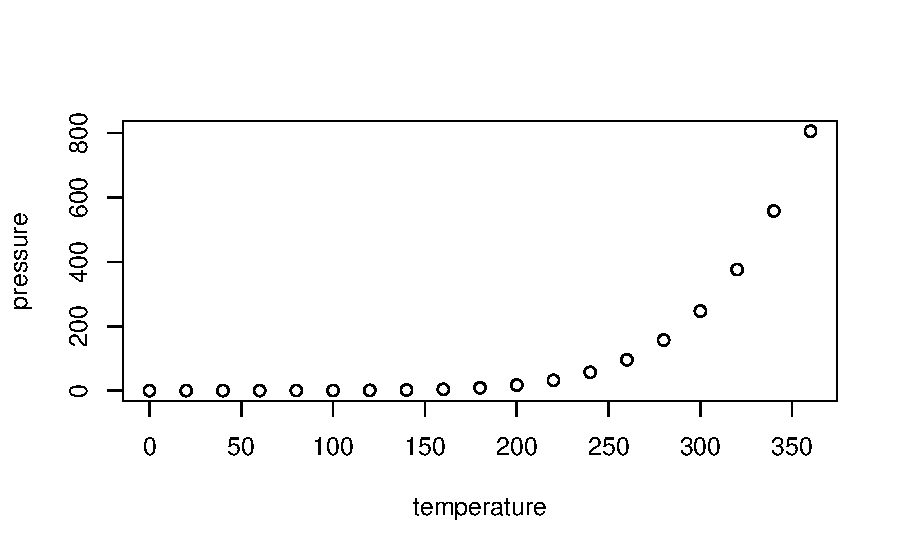
\includegraphics[width=0.7\linewidth]{Foundations_of_Program_Evaluation_files/figure-latex/pressure-1} \end{center}

Note that the \texttt{echo\ =\ FALSE} parameter was added to the code
chunk to prevent printing of the R code that generated the plot.

\hypertarget{program-impact}{%
\chapter{Program Impact}\label{program-impact}}

\hypertarget{why-do-we-use-statistical-models-for-program-evaluation}{%
\subsection{Why do we use statistical models for program
evaluation?}\label{why-do-we-use-statistical-models-for-program-evaluation}}

In unit 1 we introduced the general purpose of statistics and
quantitative methods

In unit 2 we will provide a more formal definition of how statistics is
used and what it can tell us about a program

\hypertarget{reminder-from-unit-1-advantages-of-statistical-evaluation}{%
\subsection{Reminder from Unit 1: Advantages of Statistical
Evaluation}\label{reminder-from-unit-1-advantages-of-statistical-evaluation}}

\begin{itemize}
\tightlist
\item
  Statistical models can be used with to analyze data that will show the
  quality, program impact, and where the impact occurs.
\item
  Quantitative and statistical analysis can attempt to give an unbiased
  evaluation. It can provide us with outcomes associated with
  probabilities, level of confidence, and the size of the effect. It can
  also provide information about the specific relationship between the
  program, the effect, and the impact.
\item
  Variables can be used to represent the program and its effect.
\end{itemize}

\hypertarget{the-regression-equation}{%
\section{The Regression Equation}\label{the-regression-equation}}

In unit 1 we saw that the regression line is represented by a linear
equation (Eq. 1.1). We also saw regression coefficients, often
represented by the upper case Greek letter Beta, show the slope of the
regression line. In this case the slope is Beta with a subscript of 1.
Here we only have up to \(B_{1}\). This means that there is only one
independent variable. Over next few weeks we will begin to see that we
can have more than on independent variable represented by
\(B_{1}, B_{2}, B_{3},...B_{i}\).

(Eq. 2.1) Regression Equation: \(Y = B_{0} + B_{1}X_{1}\)

The Beta with a subscript 0, (\(B_{0}\)), shows the intercept or where
the regression line crosses the horizontal axis, Eq 2.1. How can we
interpret this? If the value of \(x_1\) is 0 for a data point then
\(B_{1}\) is multiplied by 0, which would make \(B_{1}X_1 = B_{1}0 = 0\)
Because it is equal to zero all that remains is Eq 2.2.

(Eq. 2.1) Regression Equation: \(Y = B_{0} + B_{1}X_{1}\)

(Eq. 2.2) Intercept of Regression Equation: \(Y = B_{0}\)

\hypertarget{hypothetical-example-of-interpreting-the-regression-equation}{%
\subsection{Hypothetical Example of Interpreting the Regression
Equation}\label{hypothetical-example-of-interpreting-the-regression-equation}}

A manager may want to increase productivity of the employees by
implementing a new or altered program in the organization. There may be
many ways that this could happen, such as better technologies,
implementing work teams, or creating a better work environment. The
manager proposes a simple solution: increase pay. Therefore, the manager
believes that employees will be more productive with more pay.

The manager implements the pay raise and the employees are very
satisfied with the increased income. Everything seems to be going well,
but how does the manager know if the increased pay was associated with
increased productivity. In other words: did the program work? The
manager decided to simply compare raw productivity data would not lead
to enough confidence that it was successful. The solution is using
statistical methods for evaluation.

Recall that program evaluation can be interpreted as a blackbox model
(Fig. 2.1) with inputs and outcomes.

(Fig. 2.1) 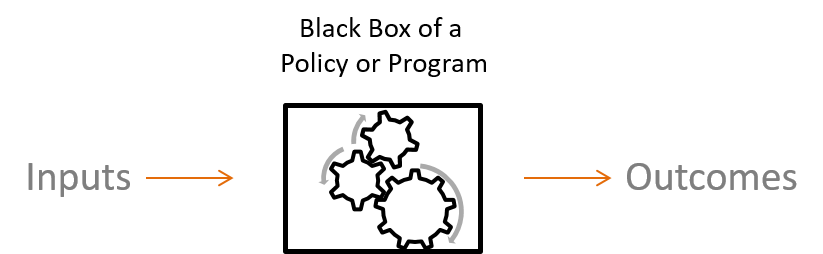
\includegraphics{figures/Input_Output_Blackbox.png}

In this case there are inputs of pay raise and outcomes of productivity
levels.

(Fig. 2.2) 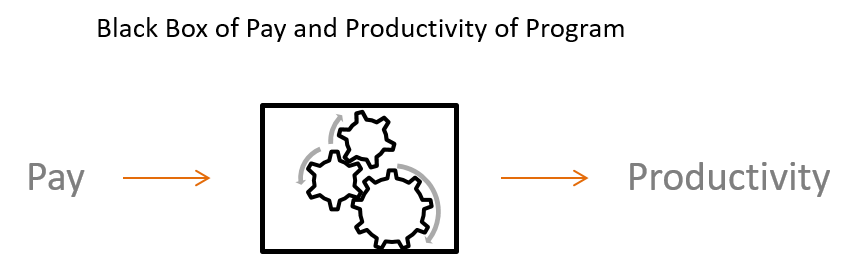
\includegraphics{figures/Pay_Productivity_Blackbox.png}

Because the manager has inputs (pay raise) and outputs (productivity)
the manager can use these to run a regression analysis.

(Eq. 2.3) Regression Eq: \(Productivity = B_{0} + B_{1}Pay Raise\)

The manager ran the regression analyis and the results show that
\(B_{0} = 50\) units of productivity and that \(B_{1} = 5\).

(Eq. 2.4) Regression Eq: \(Productivity = 50 + 5Pay Raise\)

How should the manager interpent these results? Because \(B_{0}\) is 50
it means that this is the expected productivity if there was no pay
raise. Because \(B_{1}\) is 5 it means that for each unit or dollar of a
pay raise you would expect productivity to increase by 5 units.

(Eq. 2.4) Regression Eq: \(Productivity = 50 + 5Pay Raise\)

\hypertarget{confidence-intervals}{%
\section{Confidence Intervals}\label{confidence-intervals}}

How can we be confident of our estimate of program impact?

From the example we saw that for each dollar we expect to see an
increase of 5 units of productivity. Does this mean that for every
employee each dollar of pay raise translates into 5 unit of
productivity? That would mean we would be perfectly confident that the
regression equation describes each employee perfectly. Therefore the
regression equation would resemble Fig. 2.3.

\begin{figure}

{\centering 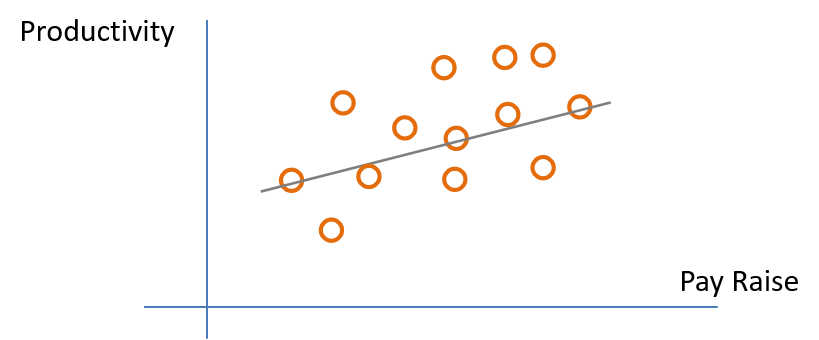
\includegraphics[width=0.328\linewidth]{figures/Pay_Productivity_With_Variance} 

}

\caption{The variance of pay productivity}\label{fig:pay-variance}
\end{figure}

However, in the real world people are all different and there is
variance in how the pay raise will impact productivity for each
individule employee. Fig. 2.4 shows that some employees have smaller
increase in prodcutivity for a dollar of pay rais and some a larger
increase.

In statistics we can use confidence intervals. Confidence intervals tell
us if we repeat an experiment many times we would expect a certain
percentage of the experiments to contain the true mean in the confidence
interval. Often people use 95\% confidence intervals. Therefore, if the
experiment is repeated 100 times we would expect 95 of those experiments
to contain the true mean within the confidence interval.

This also applies to regression. At the 95\% level if the experiment is
repeated 100 times we would expect 95 of those experiments to contain
the true \(B\) or regresion slop within the confidence interval. Later
we will see how confidence intervals are calculated, but in order to
calculate the confidence interval you must first calculate the standard
error or \(s\).

\hypertarget{confidence-intervals-for-hypothesis-testing}{%
\section{Confidence Intervals For Hypothesis
Testing}\label{confidence-intervals-for-hypothesis-testing}}

Fig. 2.5 shows a visualization of using confidence to test the
hypothesis that \(B_{1}\) for pay raise is significantly greater than
the true population \(B\), (A), or not significantly greater, (B), or
Significantly less, (C). For A and C the confidence interval does not
contain the null or true population \(B\) and therefore A shows
\(B_{1}\) significantly greater than the true population \(B\) and C
significanly less than the true population \(B\). However, because in B
the confidence interval includes the null of the true population \(B\)
there is no significant difference.

\begin{figure}

{\centering 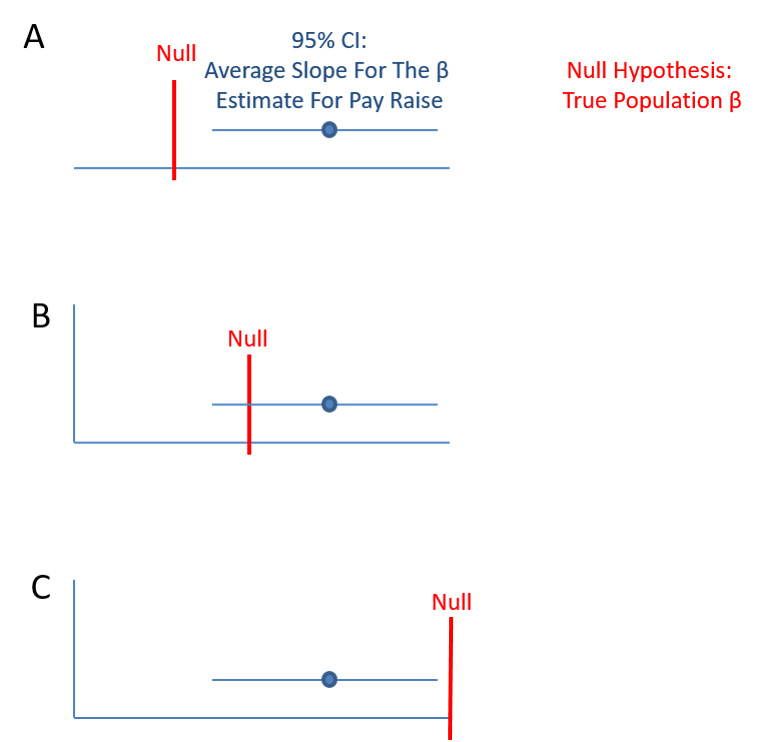
\includegraphics[width=0.5\linewidth]{figures/Confidence_Interval_Examples_B_Pay_Raise} 

}

\caption{Confidence interval of pay raises}\label{fig:pay-conf-int}
\end{figure}

\hypertarget{the-standard-error}{%
\section{The Standard Error}\label{the-standard-error}}

The standard deviation and variance are closely related. The standard
deviation essentially shows the average distance between each data point
and the mean. The standard error is simply a standard deviation used for
the sample mean or the \(B\) estimated from the sample. First we will
review the variance and standard deviation.

\hypertarget{the-variance-and-standard-deviation-of-the-mean}{%
\section{The Variance and Standard Deviation Of The
Mean}\label{the-variance-and-standard-deviation-of-the-mean}}

Eq.2.6

Eq.2.7

Eq. 2.6 shows the equation for calculating the variance.
\(\sigma^2_{x}\) is the symbol for the variance. \(\bar{x}\) is the
sample mean and \(x_{i}\) is each individual data point. Therefore,
\(x_{i}\) - \(\bar{x}\) is the size of the deviation of each data point
from the mean. The subscript \(i\) stands for index, therefore \(x_{1}\)
is the first data point. \(\Sigma\) represents the summation. Therefore,
\(\Sigma(x_{i} - \bar{x})\) is the summation of the deviation of each
data point from the mean. \(n\) is the sample size or number of data
points.

When thinking about the variance formula, why not just use the average
of the summation of the deviations of each data point? Because the mean
will be the center of the data, the sum of deviations will always equal
0. Therefore, if the deviations are squared the deviations all become
positive.

Because the variance uses squared deviation it is not in the same units
a the data points or the mean. The solution is to take the square root
of the variance, Eq. 2.7, which is called the standard deviation or
\(\sigma\). This puts the variance into the same units as the data
points and the mean. In addition, it is easier to interpret.

\hypertarget{hand-calculation-of-the-variance}{%
\subsection{Hand Calculation Of The
Variance}\label{hand-calculation-of-the-variance}}

Below shows how to calculate the variance by hand using Eq. 2.6. The
data set shows the grades of 5 students of a quiz with a maximum of 10
points. The entire data set is represented by \(X\).

\(X = [10, 8, 9, 6, 10]\)

First calculate the deviation from the mean for each data point.

\(10 - 8.6 = 1.4\)

\(8 - 8.6 = -0.6\)

\(9 - 8.6 = .4\)

\(6 - 8.6 = -2.6\)

\(10 - 8.6 = 1.4\)

The second step is to square each deviation from the mean.

\(1.4^2 = 1.96\)

\(-.6^2 = .36\)

\(.4^2 = .16\)

\(-2.6^2 = 6.76\)

\(1.4^2 = 1.96\)

The third step is tha sum or add the squared deviations from the mean.
This is called the sum of the squared deviations.

\(\Sigma(x_{i} - \bar{x})^2) = 1.96 + .36 + .16 + 6.76 + 1.96 = 11.2\)

The fourth step is to calculate the sample size minus 1.

\(5 - 1 = 4\)

The final step is to divide the sum of squared deviations by the sample
size minus 1.

\(\sigma^2 = \Sigma(x_{i} - \bar{x})^2)/(n-1)\)

\(\sigma^2 = 11.2/4 = 2.8\)

To calculate the standard deviation we simply take the square root of
the variance or 2.8.

\(\sigma = \sqrt{\sigma^2} = \sqrt{2.8} =1.673\)

\hypertarget{the-standard-error-of-the-sample-mean}{%
\section{The Standard Error Of The Sample
Mean}\label{the-standard-error-of-the-sample-mean}}

Recall that the standard error is used when we do not know the true
population standard deviation and only obtain a standard deviation of a
sample. One very interesting fact is that the distribution of the means
of each sample converges to a normal distribution as the number of
samples become very large. This is refered to as a sampling
distribution. The concept that the sampling distributions of the means
approaches a normal distribution is called the Central Limit Theorem.
Because of the Central Limit Theorem the mean and standard error are our
best estimates of the population statistics even though we only have one
sample. Therefore, we will use the standard error instead of the
standard deviation when we conduct inferential statistics from a sample.

\hypertarget{calculating-the-standard-error-of-the-mean}{%
\subsection{Calculating The Standard Error Of The
Mean}\label{calculating-the-standard-error-of-the-mean}}

Eq. 2.8 shows the standard error denoted by \(SE_{\bar{x}}\). This is
the formual that we will used for statistical analyses, such as
confidence intervals.

Eq. 2.8

\begin{figure}

{\centering 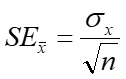
\includegraphics[width=0.328\linewidth]{figures/Standard_Error_Mean_Equation} 

}

\caption{Standard Error of the Mean}\label{fig:std-err-mean}
\end{figure}

\hypertarget{hand-calculating-the-mean-and-standard-error-of-samples.}{%
\subsection{Hand Calculating The Mean And Standard Error Of
Samples.}\label{hand-calculating-the-mean-and-standard-error-of-samples.}}

Recall that we calculated the variance and standard deviation previously
with 5 data points.If those 5 data points are the population, we can
take substes of those 5 data points as samples. Below are all the
possible samples of 3 data points.

Sample Data Sets:

\(X_{1} = [10, 8, 9]\) \(X_{2} = [10, 9, 6]\)

\(X_{3} = [10, 6, 10]\) \(X_{4} = [8, 9, 6]\)

\(X_{5} = [8, 6, 10]\) \(X_{6} = [8, 10, 10]\)

\(X_{7} = [9, 6, 10]\) \(X_{8} = [9, 10, 10]\)

\(X_{9} = [6, 10, 10]\) \(X_{10} = [6, 10, 8]\)

\hypertarget{calculating-the-standard-error}{%
\subsection{Calculating The Standard
Error}\label{calculating-the-standard-error}}

The first step is to calculate the standard deviations for each data
set. We have alreatdy calculated the standard deviation by had
previously. Therefore, the standard deviations are provided below.

\(X_{1} = 1\) \(X_{2} = 2.08\)

\(X_{3} = 2.31\) \(X_{4} =1.53\)

\(X_{5} = 2\) \(X_{6} = 1.15\)

\(X_{7} = 2.08\) \(X_{8} = .578\)

\(X_{9} = 2.31\) \(X_{10} = 2\)

The final step is to divide the standard deviations by the sqare root of
n or the sample size. For each data set the sample size is 3.

\(1/\sqrt(3) = .58\) \(2.08/\sqrt(3)\)

\(2.31/\sqrt(3) = 1.33\) \(1.53/\sqrt(3) = .88\)

\(2/\sqrt(3) = 1.55\) \(1.15/\sqrt(3) = .67\)

\(2.08/\sqrt(3) = 1.20\) \(.578/\sqrt(3) = .33\)

\(2.31/\sqrt(3) = 1.33\) \(2/\sqrt(3) = 1.55\)

\hypertarget{recap-of-the-standard-error}{%
\subsection{Recap Of The Standard
Error}\label{recap-of-the-standard-error}}

Conceptually both the standard deviation and the standard error are
identical (both measure the `average' error we expect when we make a
guess about the population statistic using a sample statistic, and the
formula for the confidence interval will be the same no matter which we
use).

The formula for the standard error for each sample statistic has been
derived by mathematicians, and provides the theoretical foundations for
inferential statistic. We don't have to take multiple samples to
calculate the average error directly. Statistical theory has already
established the relationship between descriptive statistics of a sample
and the standard error.

\hypertarget{summary-what-we-covered-in-this-unit}{%
\section{Summary: What we covered in this
unit}\label{summary-what-we-covered-in-this-unit}}

\begin{itemize}
\item
  We introduced the regression model and how to interpret the slope of
  the program and the impact on the outcome.
\item
  We introduced how to know if there is confidence in a program and the
  concept of confidence intervals.
\item
  We introduced the standard error and when we use it rather than the
  standard diviation.
\item
  We calculated step-by-step the variance, the standard deviation, and
  the standard error.
\end{itemize}

\hypertarget{looking-ahead}{%
\subsection{Looking Ahead}\label{looking-ahead}}

\begin{itemize}
\item
  We will cover the interpretation of the standard error.
\item
  We will cover the details of calculating confidence intervals.
\item
  We will cover the regression model in more detail.
\end{itemize}

\hypertarget{confidence-intervals-1}{%
\chapter{Confidence Intervals}\label{confidence-intervals-1}}

\textbf{What is the standard error and how is it used?}

In unit 2 we showed that the standard error is a type of standard
deviation. This describes how variable the data is and how far the data
is from the mean.

The important difference is that the standard error is used when there
is an inferential statistical analysis using a sample and the true
population statistics are not known.

Confidence interval tell us how confident we can be that the there is a
difference between the null hypothesis.

\hypertarget{how-the-size-of-the-standard-error-represents-confidence}{%
\section{How The Size Of The Standard Error Represents
Confidence}\label{how-the-size-of-the-standard-error-represents-confidence}}

Recall that the standard error describes the variability of the data.
The more variable the data the less confidence there is. For example,
assume that every week you get paid very different amounts. Some weeks
you get paid a large amount, some weeks a reasonable and moderate
amount, but other weeks you get paid very little. This type of pay is
very variable. Would you have much confidence in the amount of money you
have to spend every week? Most likely you would have little confidence.
This is because the variability is so large. The standard error is
similar. Large standard error lead to less confidence. However, smaller
standard errors allow for high confidence. Next we will introduce how to
calculate standard errors followed by the details of confidence
intervals.

\hypertarget{factors-that-influence-the-size-of-the-standard-error}{%
\subsection{Factors That Influence The Size Of The Standard
Error}\label{factors-that-influence-the-size-of-the-standard-error}}

The main factor that affects the size of the standard error is the
sample size. Because the denominator of the standard error is the square
root of the sample size (Eq.3.1) as the sample size gets larger the
standard error becomes smaller.

\hypertarget{the-standard-error-of-the-mean-equation}{%
\subsection{The Standard Error Of The Mean
Equation}\label{the-standard-error-of-the-mean-equation}}

Eq. 3.1

\hypertarget{factors-that-influence-the-size-of-the-standard-error-in-regression}{%
\subsection{Factors That Influence The Size Of The Standard Error In
Regression}\label{factors-that-influence-the-size-of-the-standard-error-in-regression}}

We will discuss more details about the regression model in the next few
units. Recall that because every data point does not usually fall in a
perfect line there is usually space between each data point and the
regression line. The distance between the data point and the regression
line is called the error term or residual (Fig.3.1). One way to decrease
the size of the standard error is to add more variables.

\hypertarget{the-residual-in-regression}{%
\subsection{The Residual In
Regression}\label{the-residual-in-regression}}

Fig. 3.1

\hypertarget{factors-that-influence-the-size-of-the-standard-error-in-regression-1}{%
\subsection{Factors That Influence The Size Of The Standard Error In
Regression}\label{factors-that-influence-the-size-of-the-standard-error-in-regression-1}}

Recall that the regression slope, \(B\), describes the impact on the
dependent variable or output. It describes how many units the output
will increase or decrease for every one unit of change of the
independent variable or input. There is also a standard error of \(B\).
The calculation is similar. Eq. 3.1-3.4 show the formulas to calculate
the variance and standard deviation of the slope. In Eq. 3.3 \(SSE\) is
the sum of squared error term. It is analogous to the sum of the
deviation of the sum of the deviations from the each data point and the
regression line. Eq. 3.5 Shows the formula for the standard error of the
regression slope. Just as with the standard error of the mean you must
first calculate the variance.

\hypertarget{the-variance-and-standard-deviation-of-the-regression-slope-equation}{%
\subsection{The Variance And Standard Deviation Of The Regression Slope
Equation}\label{the-variance-and-standard-deviation-of-the-regression-slope-equation}}

Eq. 3.2 \(SSE = ({\hat{y}_i} - \bar{y})^2\)

Eq. 3.3

Eq. 3.4

\hypertarget{the-standard-error-of-the-regression-slope-equation}{%
\subsection{The Standard Error Of The Regression Slope
Equation}\label{the-standard-error-of-the-regression-slope-equation}}

Eq. 3.5

Two other ways to decrease the size of the standard error are (1)
increase the sample size and (2) to increase the variance of \(x\).
Increasing the sample size will decrease the variance of the regression
slope by increasing the denominator of the variance (Eq.3.5). Similarly,
increasing the variance of \(x\) will increase the denominator of the
standard error of the slope leading to a smaller \(SE_b\).

\hypertarget{standard-errors-and-confidence-intervals}{%
\section{Standard Errors And Confidence
Intervals}\label{standard-errors-and-confidence-intervals}}

Recall that Confidence intervals tell us if we repeat an experiment many
times we would expect a certain percentage of the experiments to contain
the true mean in the confidence interval. Often people use 95\%
confidence intervals.

If the experiment is repeated 100 times we would expect 95 of those
experiments to contain the true mean within the confidence interval.

In order to calculate confidence intervals we must know how variable the
data are. This is estimated by the standard error. We can now use the
standard error to calculate the confidence interval

\hypertarget{calculating-the-confidence-interval-of-the-mean}{%
\subsection{Calculating The Confidence Interval Of The
Mean}\label{calculating-the-confidence-interval-of-the-mean}}

Recall that the standard error is a type of standard deviation. However,
it is used when we are calculating statistics from a sample and do not
know the true population statistics. The formulas and equations are very
related and similar. You likely have seen in earlier statistics courses
how to calculate the t-statistic.

The t-statistic is used to determine the probability that you would get
the results that you obtain from your sample if the results were due to
random chance. In other words, it is very similar to confidence
intervals. If you are interested in a probability or p-value of less
than 5\% or .05 to be significant then a t-statistic that shows the
p-value is less than .05 you believe that the results were not due to
random chance, rather they were due because there is a true difference
between the mean of your sample and the population mean. For example, a
t-statistic that shows a p-value of less than .05 in a study where you
wanted to know if a drug worked better than a placebo you would infer
that the results of the drug were not due to random chance.

The t-statistic is integrally involved in the calculation of confidence
intervals. One reason is that, as with t-tests, we have a probability
value or in this case a confidence level. In calculating the t-statistic
for the confidence interval we must know the degrees of freedom. A
t-statistic for the mean has \(n-1\) degrees of freedom or the sample
size minus 1. The t-statistic for the regression slope, \(B\), the
degrees of freedom are \(n-k-1\) or the sample size minus the number of
regression paramaters, \(B\)'s, minus 1.

\hypertarget{the-regression-residual}{%
\chapter{The Regression Residual}\label{the-regression-residual}}

\textbf{Viewing The Regression Line As A Conditional Average}

In statistics, conditional basically means if you know the value of one
variable you either know or can estimate the value of another variable.
In other words, if you tell me the level of \(x\), I can tell you the
average \(y\) for someone with that level of \(x\). In terms of the
regression x is the value of the input or independent variable of a
program and \(y\) is the outcome or dependent variable of the program.
Therefore, \(y\) is dependent or conditional on \(x\).

\hypertarget{regression-residuals-and-errors}{%
\section{Regression Residuals And
Errors}\label{regression-residuals-and-errors}}

Recall the example of pay raise and productivity. In the real wold
people vary. The regression line gives us the best linear fit or
prediction of what productivity or \(y\) will be if we know the pay
raise or \(x\). Therefore \(y\) is conditional on \(x\). However, the
true values of productivity conditional on each person's productivity
varies by person and therefore varies around the regression line instead
of being perfectly on it. (Fig. 4.1)

Fig. 4.1 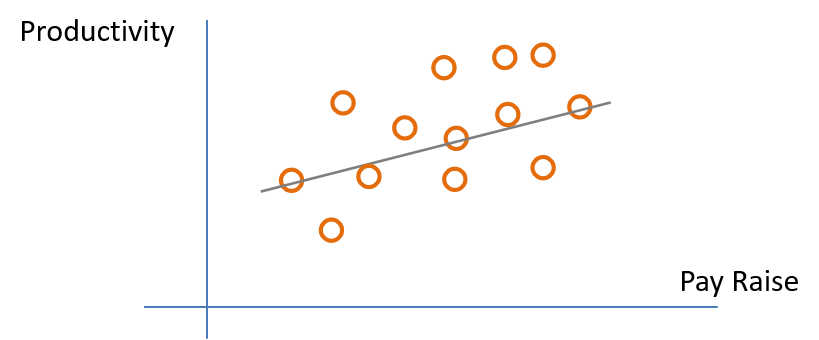
\includegraphics{figures/Pay_Productivity_With_Variance.png}

As in Fig. 4.1, the data will cluster around the regression line, but
not on it. The residual is calculated from the actual value of \(y\)
minus the predicted value of \(y\) or \(\hat{y}\), which is a point on
the regression line. (Fig. 4.2)

\hypertarget{the-residual-in-regression-1}{%
\section{The Residual In
Regression}\label{the-residual-in-regression-1}}

Fig. 4.2

\hypertarget{interpreting-and-using-the-residual-in-regression}{%
\subsection{Interpreting And Using The Residual In
Regression}\label{interpreting-and-using-the-residual-in-regression}}

The regression line tells us our best linear estimate of \(y\)
conditional on \(x\). This can also be said as \(y\) given \(x\), which
is represented mathematically as \({y|x}\). However, because the actual
data usually cluster around the regression line each data point likely
has a regression residual.

The regression residual can be either positive or negative. In other
words, some data points will be above the regression line leading to a
positive residual and some data points will be below the regression line
leading to a negative residual.

A good example of residuals in regression is ``The Math of Cities''.
This example is based on data from the Census. It basically shows that
the size of the city is related to productivity. For this study they
used the number of patents as a measure of productivity. This is
reasonable because it is a measure of ingenuity and the creation of new
ideas and products. To listen to the researchers go to
\url{https://www.wnycstudios.org/story/96043-its-alive/} and listen to
the time 12:30-17:30.

\hypertarget{how-the-residual-describes-over-performing-and-under-performing}{%
\subsection{How The Residual Describes Over-performing and
Under-performing}\label{how-the-residual-describes-over-performing-and-under-performing}}

Let us consider the example of ``The Math of Cities''. What does it mean
to be over-performing or under-performing relative to city size? If a
city over-performs relative to the regression line the number of patents
or productivity will lead to a positive residual. If you under-perform
relative to the regression line the number of patents or productivity
will lead to a negative residual. Fig. 4.3 shows the regression line and
how some cities are above the line and over performing and some below
and under-performing.

Fig. 4.3

As we have noted residuals can be positive or negative, and reflect
over-performing and under-performing in ``The Math and Cities'' example.
Fig. 4.4 shows the residuals represented by the red line connecting each
data point and the regression line. These red vertical lines represent
the distance between the data points and the regression line. The
positive residuals are the the red lines above the regression line and
the negative residuals are the red lines below the regression line.
\({e}\) in the regression equation represents the error or the
regression residual.

Fig.4.4

\hypertarget{how-do-we-know-the-best-fitting-regression-line-for-our-data}{%
\section{How Do We Know The Best Fitting Regression Line For Our
Data}\label{how-do-we-know-the-best-fitting-regression-line-for-our-data}}

Finding the best fitting regression line uses mathematics that can be
calculated by hand. Luckily computers identify the regression line based
upon the criteria of ``line of best fit'' for the data. In most cases,
this means that we are finding the line that minimizes the distance
between the line and all data points, i.e.~minimizing the error in the
model. These errors are the red lines representing the regression
residuals (Fig. 4.4).

\hypertarget{the-calculation-of-the-regression-line}{%
\subsection{The Calculation Of The Regression
Line}\label{the-calculation-of-the-regression-line}}

Calculating the regression line and slope coefficients must find the
best fitting line. Therefore, it would be a better fit if there is
minimum error or residuals for the entire set of data points. Just as we
did with the variance, we could not use the absolute error, but rather
we squared the deviations from the mean. To calculate the regression
line we will also need to square the error or residuals.

Eq. 4.1 shows the regression line that we have studied previously. This
equation has a subscript \({i}\) for \({x}\) and \({y}\). This subscript
represents each data point. Therefore, we have a specific value for each
\(y_{i}\) or the dependent variable and for each \(x_{i}\), which is
taken directly from data that was collected.

Eq. 4.1

\(y_{i} = B_{0} + B_{1}x_{i} + e_{i}\)

To calculate the best fitting regression line we must minimize the error
for the entire data set. Therefore, we will minimize the sum of squared
errors or residuals. With a little algebra Eq. 4.1 can be rearranged to
give you the equation in terms of the error term/residual with it on the
left side of Eq. 4.2. This is essentially solving for the error term
\({e}\). The next step is to sum the squared errors/residuals of each
data point. This is shown in Eq. 4.2.

Eq. 4.2

\(e_{i} = y_{i} - B_{0} - B_{1}x_{i}\)

Eq. 4.3

\(\Sigma(e_{i} = y_{i} - B_{0} - B_{1}x_{i})^2\)

The next step is to minimize Eq. 4.3 or the sum of squares of the
residuals. This requires calculus and is beyond the scope of this
course. Once Eq. 4.3 is minimized you can calculate the intercept and
slope coefficients of the regression line \(B_{0}\) and \(B_{1}\). This
is called the ordinary least square regression or OLS. Statistical
packages, such as R and others, can give you the OLS regression line.

\hypertarget{implications-of-squaring-residuals}{%
\subsection{Implications Of Squaring
Residuals}\label{implications-of-squaring-residuals}}

Using sum of squares in both variance and calculating regression lines
has important consequences in regard to misinterpreting the meaning of
the sum of squares. If we think back to the variance and standard
deviation of the mean, because the variance is in terms of squared
deviation each unit of increase in the data leads to a squared
difference. This leads to an increasingly larger increase in variance
for each unit a data point is from the mean.

Her are examples of squared deviations leading to misinterpreting the
absolute deviations. These are the results of squaring each deviation
from the mean. If a data point deviates \(1\) point from the mean then
\(1^2\) is \(1\). If a data point is \(2\) units from the mean then
\(2^2\) is \(4\). If a data point is \(3\) units from the mean then
\(3^2\) is \(9\). This leads to the squared deviations from the mean
increasing much more quickly than the absolute deviations. In this
example we can see this by noticing \(2^2\) being \(4\) times a
deviation of \(1\) and \(3^2\) being \(9\) times a deviation of \(1\).
The solution was to take the square root to put the squared units into
the same units as the original data. This is the same with the squared
residuals. This is important when considering outliers. Outliers using
squared residuals can have an extreme effect on the analysis.

\textbf{The Regression Line Passes Through Both The Mean Of Y And Mean
Of X}

Once the sum of the squared residuals is minimized to calculate the
regression line the results give the equation for the intercept
\(B_{0}\) (Eq. 4.4) and the equation for the regression slope \(B_{1}\)
(Eq. 4.5). Remember that the ``hat'' over the \(B's\) represent the
fitted or estimates and the ``bar'' over \(x\) and \(y\) represent the
mean. This will imply that the regression line passes through the mean
of \(x\) and the mean of \(y\).

\hypertarget{the-regression-coefficient-equations-estimates}{%
\section{The Regression Coefficient Equations
Estimates}\label{the-regression-coefficient-equations-estimates}}

Eq. 4.4

\(\hat{B_{0}} = \bar{y}-\hat{B_1}\bar{x}\)

Eq. 4.5

\(\hat{B_{1}} = (\Sigma(x_{i}-\bar{x})({y}_{i}-\bar{y}))/(\Sigma(x_{i}-\bar{x})^2\)

\hypertarget{looking-forward}{%
\section{Looking Forward}\label{looking-forward}}

\begin{enumerate}
\def\labelenumi{\arabic{enumi}.}
\item
  We will explore the regression slope further.
\item
  We will discuss how there is variability and a standard error of the
  regression slope as there is with the mean.
\item
  We will also discuss how variables vary together, which can be
  measured by the covariance.
\end{enumerate}

\hypertarget{figure-example}{%
\section{Figure Example}\label{figure-example}}

\begin{Shaded}
\begin{Highlighting}[]

\KeywordTok{plot}\NormalTok{( }\KeywordTok{rnorm}\NormalTok{(}\DecValTok{50}\NormalTok{), }\KeywordTok{rnorm}\NormalTok{(}\DecValTok{50}\NormalTok{), }\DataTypeTok{cex=}\FloatTok{0.5}\OperatorTok{*}\KeywordTok{sample}\NormalTok{(}\DecValTok{1}\OperatorTok{:}\DecValTok{5}\NormalTok{,}\DecValTok{25}\NormalTok{,T), }\DataTypeTok{bty=}\StringTok{"n"}\NormalTok{, }\DataTypeTok{pch=}\DecValTok{19}\NormalTok{, }\DataTypeTok{col=}\StringTok{"gray"}\NormalTok{ )}
\end{Highlighting}
\end{Shaded}

\begin{figure}

{\centering 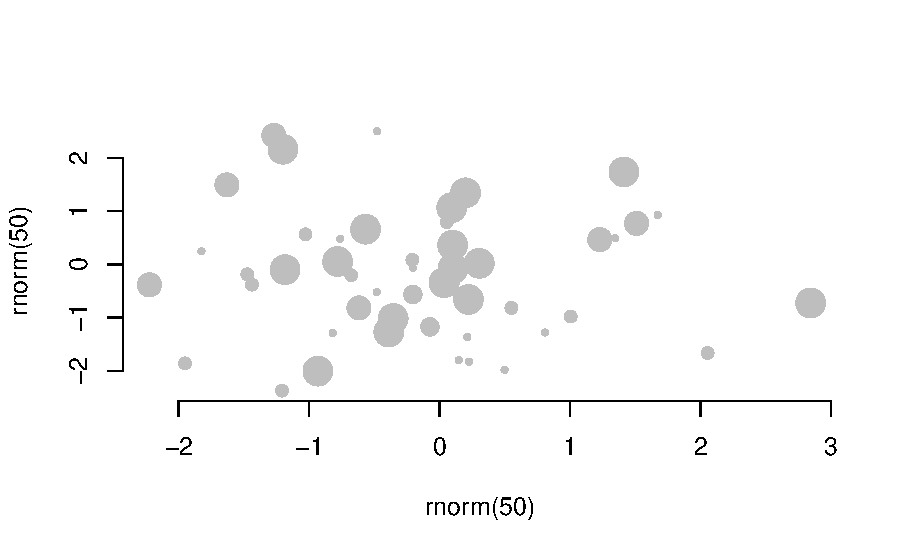
\includegraphics[width=0.7\linewidth]{Foundations_of_Program_Evaluation_files/figure-latex/fig1-1} 

}

\caption{Here is a Figure Caption}\label{fig:fig1}
\end{figure}

In \ref{fig:fig1} we see examples of plotting in R, and another example
in \ref{fig:fig2}.

\begin{Shaded}
\begin{Highlighting}[]

\KeywordTok{plot}\NormalTok{( }\KeywordTok{rnorm}\NormalTok{(}\DecValTok{50}\NormalTok{), }\KeywordTok{rnorm}\NormalTok{(}\DecValTok{50}\NormalTok{), }\DataTypeTok{cex=}\FloatTok{0.5}\OperatorTok{*}\KeywordTok{sample}\NormalTok{(}\DecValTok{1}\OperatorTok{:}\DecValTok{5}\NormalTok{,}\DecValTok{25}\NormalTok{,T), }\DataTypeTok{bty=}\StringTok{"n"}\NormalTok{, }\DataTypeTok{pch=}\DecValTok{19}\NormalTok{, }\DataTypeTok{col=}\StringTok{"firebrick"}\NormalTok{ )}
\end{Highlighting}
\end{Shaded}

\begin{figure}

{\centering 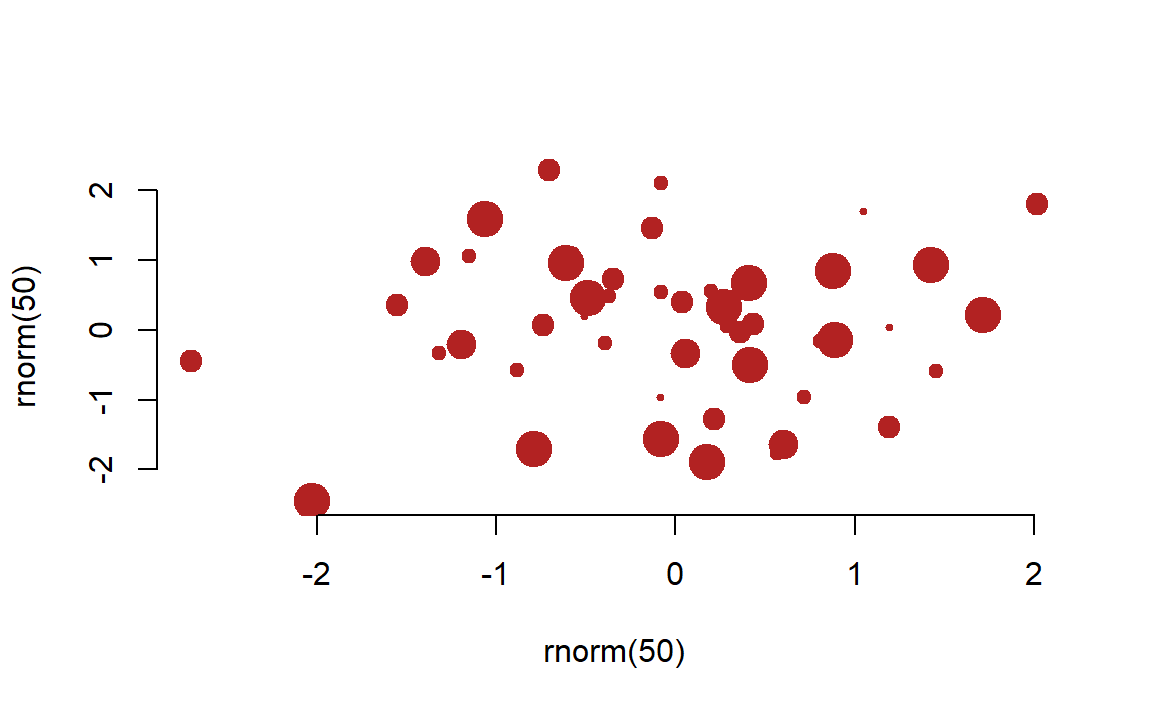
\includegraphics[width=0.7\linewidth]{Foundations_of_Program_Evaluation_files/figure-latex/fig2-1} 

}

\caption{plotting example}\label{fig:fig2}
\end{figure}

\hypertarget{the-regression-slope}{%
\chapter{The Regression Slope}\label{the-regression-slope}}

\hypertarget{variance-revisited}{%
\section{Variance Revisited}\label{variance-revisited}}

Recall from Unit 2 we discussed the variability and variance of the
data. We therefore are intersted in how the data is spread out from the
mean of the data. To assess how the data is spread out from the mean we
want a measure for how spread out or how the data deviates from the mean
\(\bar{x}\) This is accomplished by using the following calculation:
\(\Sigma(x_{i} - \bar{x})\), which is the summation of the deviation of
each data point from the mean. The complete formula for calculating the
variance is Eq. 5.1

Eq. 5.1 \(\sigma^2 = \Sigma(x_{i} - \bar{x})^2)/(n-1)\)

We also saw that if you add all of the deviations from the mean, the
distance from the mean of each data point, it will always be \(0\). To
solve this problem of the sum of the deviations being \(0\) we squared
each deviation, which you can see in Eq. 5.1.

\hypertarget{the-standard-deviation-revisited}{%
\section{The Standard Deviation
Revisited}\label{the-standard-deviation-revisited}}

Recall that we calculated the standard deviation by taking the square
root of the variance. This is necessary because the squared deviations
from the mean are in squared units. However, the original data and the
mean are not in squared units. Taking the square root of the variance it
puts the standard deviation in the original units.

\hypertarget{squared-residuals}{%
\subsection{Squared Residuals}\label{squared-residuals}}

Related to the variace, we minimized the sum of the squared residuals,
or the distance of each data point from the regression line. This will
give us the best estimation for the regression line.

\hypertarget{covariance}{%
\section{Covariance}\label{covariance}}

So far we have discussed how the data varies around the mean and varies
around the regression line. Often we are interested in how two variables
vary together. In otherwords, as one variable increase does the other
variable increase or decrease. How two variables vary with each other is
called the covariance. This is related to regression slopes. If the
regression slope is positive then as the independent variable increases
the dependent variable increases. If the regression slope is negative
then as the independent variable increases the dependent variable
decreases.

\hypertarget{calculating-the-covariance}{%
\subsection{Calculating The
Covariance}\label{calculating-the-covariance}}

The equation for the covariance will look similar to that of the
variance. With the variance we calculated the sum of the squared
deviations from the mean. However, with covariance we have two
variables. For the covariance we now calculate the sum of the deviations
of the two variables multiplied together, variable \(1\) or \(x\) and
variable \(2\) or \(y\), Eq. 5.2. While similar to the next step in the
variance, for the covariance we now add the multiplied deviations of
\(x\) and \(y\), Eq. 5.3.

Eq. 5.2

\((x_{i} - \bar{x})(y_{i} - \bar{y})\)

Eq. 5.3

\(\Sigma(x_{i} - \bar{x})(y_{i} - \bar{y})\)

Finally we divide by \(n-1\), or the sample size minus 1. Eq. 5.4.
\(cov(x,y)\) stands for the covariance. Let us look at Eq. 5.4 more
closely. A positive number multiplied by a positive number will result
in a positive number. Therefore if \((x_{i} - \bar{x})\) and
\((y_{i} - \bar{y})\) are either both positive or both negative then the
numerator and thus the covariance will be positive. Alternatively, if
\((x_{i} - \bar{x})\) is positive and \((y_{i} - \bar{y})\) is negative
than the numerator and thus the covariance will be negative. The third
possibility is if \((x_{i} - \bar{x})\) is negative and
\((y_{i} - \bar{y})\) is positive than the numerator and thus the
covariance will be also be negative.

Eq. 5.4

\(cov(x,y)=\Sigma(x_{i} - \bar{x})(y_{i} - \bar{y})/n-1\)

We can use the covariance to calculate the correlation between two
variables. Corrlation measures the strength of the linear relationship
and the direction between two variables. Suppose we were interested in
how class size, the independent variable, is related to test scores, the
dependent variable. If there is a positive covariance and correlation
between the the two variables will increase from bottom left to upper
right in a plot, Fig. 5.1.

\hypertarget{positive-correlation}{%
\subsection{Positive Correlation}\label{positive-correlation}}

Fig. 5.1

\hypertarget{negative-corrleation}{%
\subsection{Negative Corrleation}\label{negative-corrleation}}

If there is a negative covariance and correlation between the the two
variables will decrease from top left to bottom right in a plot,

Fig. 5.2

\hypertarget{low-correlation}{%
\subsection{Low Correlation}\label{low-correlation}}

If there is a low to no covariance and correlation (the variables are
unrelated) between the the two variables will appear randomly scatterd
in the plot with no upward or downward to the right, Fig. 5.3. There are
two other possibilitties. If the plot is either arranged in a vertical
or horizontal pattern then there is also no correlation. This is because
the vertical plot means as \(y\) increases then \(x\) does not change
and the horizontal plot means as \(x\)increases \(y\) does not change.

Correlations are always between \(-1\) and \(+1\). If the the
correlation is closer to \(1\), then the correlation is positive and has
a strong linear relationship. If the correlation is closer the
correlation is to \(-1\), then the correlation is negative and has a
strong linear relationship. Finally, if the correlation is closer to
\(0\), then the correlation is low and has a weak linear relationship. A
correlation of \(0\) would mean that the variables are completely
unrelated.

\hypertarget{the-slope}{%
\section{The Slope}\label{the-slope}}

Recall the equations for the covariance and variance: Eq. 5.4 and Eq.
5.1. We can divide the covariance by the variance as seen in Eq. 5.5.
With a little algebra \((n-1)\) in both the covariance and variance will
cancel out each other. This will leave us with
\([(\Sigma(x_{i} - \bar{x})(y_{i}) - \bar{y})]/[\Sigma(x_{i} - \bar{x})^2)]\).
By cancelling each \(\Sigma(x_{i} - \bar{x})\) in the numerator and
denominator we are left with the components in Eq. 5.6. This is an
intuitive formula for the slope because, if you recall from algebra the
slope of a line is the change in \(y\) divided by the change in \(x\).

Eq. 5.5
\(cov(x,y)/var(x)=[\Sigma(x_{i} - \bar{x})(y_{i} - \bar{y})/n-1]/[\Sigma(x_{i} - \bar{x})^2)/(n-1)]\)

Eq. 5.6 \((y_{i} - \bar{y})/(x_{i} - \bar{x})\)

\hypertarget{looking-ahead-1}{%
\section{Looking Ahead}\label{looking-ahead-1}}

\begin{itemize}
\item
  We will discuss how the variance can be explained with partitioning
  different variaces
\item
  We will discuss \(R^2\) or the coefficient of determination
\end{itemize}

\hypertarget{explaining-variance}{%
\chapter{Explaining Variance}\label{explaining-variance}}

The variance can be split up into components of several parts.
Intuitively, if you consider a regression model that has two independent
variables, \(x_1\) and \(x_2\). This would imply that the dependent
variable, \(y\), would have variances from two components that can help
explain how the independent variables are related to it.

Two components of the variance are the regression sum of squares, RSS,
and the error sum of squares, ESS. Eq's. 6.1 and 6.2 show the equations
that are used to calculate RSS and ESS. Finally there are the total sum
of squares, TSS, which is simply adding RSS and ESS together.

Eq. 6.1

\(RSS = \Sigma(\hat{y_i} - \bar{y})^2\)

Eq. 6.2

\(ESS = \Sigma(y_i - \hat{y_1})^2\)

Eq. 6.3

\(TSS = \Sigma(y_i - \bar{y})^2 = RSS + ESS\)

\hypertarget{r-squared}{%
\section{R-Squared}\label{r-squared}}

One important measurement in statistics and explaining the variance is
R-squared or \(R^2\). Basically \(R^2\) is the percentage of the
variance explained by independent variables or the regression model.
This can be seen in Eq. 6.4 by seeing it is simply the ratio of the
explained variance or simplified to the explained sum of squares divided
by the total sum of squares. This will always give us a value between 0
and 1, which also reflects the ratio or percentage. Because we are using
how much the regression explains the explained sum of squares is the
same as the regression sum of squares or \(RSS\).

Eq. 6.4

\(R^2 = RSS/TSS\)

Because it is a percentage, sometimes it is easier to use Eq. 6.5. This
comes directly from the factor that the ratio and percentage measured by
Eq. 6.4 must add to 1.

Eq. 6.5

\(R^2 = ESS/TSS\)

\hypertarget{hand-calculation-of-the-regression}{%
\section{Hand Calculation Of The
Regression}\label{hand-calculation-of-the-regression}}

Below shows the data you previously used to calculate the variance in
Unit 2. The data set shows the grades of 5 students of a quiz with a
maximum of 10 points. The entire data set is represented by \(Y\). This
time we are representing that data with \(Y\) because we will treat this
as the dependent variable. The data set \(X\) will now be used for the
hours spent studying for the quiz.

\(Y = [10, 8, 9, 6, 10]\)

\(X = [5, 2, 3, 3, 6]\)

As an exercise please use the data above to calculate the slope,
intercept, predicted Y, residual, and sum of squared errors for the
regression. You can use the equations we just showed and have seen
earlier. In addition show the following:

\begin{enumerate}
\def\labelenumi{\arabic{enumi}.}
\tightlist
\item
  Show that the sum of squared errors becomes the numerator in the
  standard error of the slope
\item
  Calculate the regression sum of squares (difference between observed
  and predicted value)
\item
  Calculate the total sum of squared errors \(\Sigma(y_2 - \bar{y})^2\)
  and show that this is the raw variance instead of the average variance
\item
  Calculate the R-square as RSS/TSS and 1 - ESS/TSS.
\item
  Emphasize that RSS + ESS = TSS, or explained variance plus unexplained
  variance is equal to total variance.
\end{enumerate}

\hypertarget{partitioning-the-variance-of-y}{%
\section{Partitioning The Variance Of
Y}\label{partitioning-the-variance-of-y}}

Now that we have introduced how to calculate the different sum of
squares we will discuss the partitioning of the variance. When taking
any equation you can add and subtract the same value or same additional
variable and the original equation stays the same. Eq. 6.6 shows a
generall example of this. We simply add and subtract \(C\) and therefore
does not change the result of the original equation of \(A + B\).

Eq. 6.6

\(A + B = A + C - C + B\)

Recall that part of calculating the variance involves the deviations of
the actual data from the mean. Therefore we can use the deviation as an
approximation to represent the variance. Eqq. 6.7 shows the deviation.
Just as in Eq. 6.6 we can add and subtract the value of \(\hat{y_i}\).
Eq. 6.8. This will apprimately represent the variance of \(y\).

Eq. 6.7

\(y_i - \bar{y}\)

Eq. 6.8

\(y_i - \hat{y} + \hat{y} - \bar{y}\)

If you look closely at Eq. 6.8 you can see that this is now actually a
part of the residual sum of squares, Eq. 6.9, and and the regression or
explained sum of squares, 6.10.

Eq. 6.9: Residual

\(y_i - \hat{y}\)

Eq. 6.10: Regression/Explained

\(\hat{y} - \bar{y}\)

\hypertarget{the-relationship-of-r-squared-and-partitioned-variance}{%
\subsection{The Relationship Of R-Squared And Partitioned
Variance}\label{the-relationship-of-r-squared-and-partitioned-variance}}

Because \(R^2\) is the regression or explained sum of squares devided by
the total sum of squares we can use the partitioned variance to
calculate \(R^2\). Recall that the total sum of squares is simply the
residual sum of squares plus the regression sum of squares. Therefore,
from that partition of the variance we have the regression or explaned
sum of squares and the residual sum of squares. These are all of the
components that are needed to calculate \(R^2\) with Eq. 6.4. Another
measurement is r, or the correlation. This shows how two variables
correlate positively, correlate negatively or not correlated at all.
This is related to the covariance. \(R^2\) is simply the square of r.

\hypertarget{looking-ahead-2}{%
\section{Looking Ahead}\label{looking-ahead-2}}

\begin{itemize}
\item
  We will discuss Bellentine Diagrams and how they relate to
  correlation.
\item
  We will use the diagrams to visualize the partitioning of the variance
  now that we have introduced the mathematics.
\item
  We will discuss how the variance of each variable and the size of the
  circles in the diagrams represent variance.
\end{itemize}

\hypertarget{ballentine-venn-diagrams}{%
\chapter{Ballentine Venn Diagrams}\label{ballentine-venn-diagrams}}

Diagrams, graphs, and charts can be very helpful in statistics. These
are tools that help to visually represent equations and concepts that
are used in statistics. Bellentine Venn Diagrams are a great way to many
of the concepts that we have just recently discussed by representing
them visually.

\hypertarget{concepts-that-bellentine-venn-diagrams-can-represent}{%
\subsection{Concepts That Bellentine Venn Diagrams Can
Represent}\label{concepts-that-bellentine-venn-diagrams-can-represent}}

These diagrams help show the following concepts:

-Variance (larger variance means larger circle)

-Covariance (larger covariance means more overlap between two circles)

-Residual (portion of \(Y\) that is not covered by all independent
variables)

-Explained variance (portion of the variance of \(y\) that is accounted
for by \(x\))

-R-square (ratio of the residual to total variance)

-Slope (ratio of covariance to variance of \(x\))

-Standard error (ratio of residual to variance of \(x\))

\hypertarget{variance}{%
\subsection{Variance}\label{variance}}

The Venn Diagrams very nicely show these statistical concept and the
variance is a very clear concept that is represented. Recall that
variance is how spread the data is from the mean. Therefore, we can
represent the variance with a circle and then the wider the circle is or
the larger the diameter is a larger variance. Fig. 7.1 shows that
\(x_1\) has a smaller variance than \(x_2\).

Fig. 7.1

Eq. 7.1 shows the variance of \(y\), Eq. 7.2 shows the variance of
\(x_1\), and Eq. 7.3 Shows the variance of of \(x_2\).

\(var(y) = \Sigma{(y_i} - \bar{y})^2\)

\hypertarget{covariance-1}{%
\section{Covariance}\label{covariance-1}}

The covariance is represented by the overlap of the circles in the
diagrams. Because the covariance shows how two variables relate, this
means that they share variation together and therefore must overlap. In
Fig. 7.2 you can see that \(x_1\) and \(y\) share space in the diagram
and covary together.

Fig. 7.2

You can also see that \(x_1\) and \(x_2\) overlap in Fig. 7.2. Recall
the partitioning of variance, a related topic, therefore the
\(cov(x,y) = A+B\) and the \(cov(x_1,x_2) = C+D\).

\hypertarget{correlation}{%
\section{Correlation}\label{correlation}}

Recall that the correlation involves covariance and therefore will be
reflected in a similar way in the Venn Diagrams. Fig. 7.3 shows this,
and the correlation is also what is called the standardized slope.

Fig. 7.3

This relationship between the covariance and correlation can be seen in
Eq. 7.2. The abreviation of std stands for the standard deviation.

Eq. 7.2

\(cor(x_1,y) = cov(x_1,y)/(std(x_1)std(y))\)

\hypertarget{slope}{%
\section{Slope}\label{slope}}

From your prerequisit courses in statisics you may recall that in a
normal distribution z scores are standardized scores that place
everything in units of standard deviations, which are the same because
it is 1 for each. The same can be accomplished by standardizing the
slope in a regression. Also, recall that the slope of a line is the rize
over the run, or the change in in \(y\) divided by the change in \(x\).
This can be seen in Fig. 7.4 and in Eq. 7.3.

Fig. 7.4

Eq. 7.3

\(B_1 = cov(x,y)/var(x) = A/(A+C)\)

\hypertarget{r-square-and-the-regression-residual}{%
\section{R-Square and the Regression
Residual}\label{r-square-and-the-regression-residual}}

Finally, \(R^2\) represent the percentage of the explained variance in a
regression. The Venn diagrams visually illustrate this very well. In
other words, a percentage of the explained variance would be calculated
by the ratio of the explained variance of a variable divided by the
total variance of the same variable. A similar example is if you flip a
coin 1000 times it is very likely to result in heads close to 500 times
and close to tails 500 times. To the percentage of heads would be aroung
500/1000 or \(50%\). The analogous situation for \(R^2\) can be seen in
Fig. 7.5. Also, e, or the error term is proportional to B in the
diagram.

Fig. 7.5

Eq. 7.4 shows the equation to calculate \(R^2\) and how it is
represented using the Regions of A and B in Fig. 7.5.

Eq. 7.4

\(R^2 =\) explained \(var(y)/var(y)\) is approximately \(= A/(A+B)\)

Fig. 7.6 shows two different examples of data and the calculations of
the variances of \(x\) and \(y\) in each example. You will notice that
the slopes are the same, but the data in the first example is more
spread out than the second example. This is also reflected in the larger
variance of \(y\) in the first example. The larger variance leads to a
larger residual. Because the variance and residual in the first example
are larger also leads to a smaller \(R^2\) or percentage of the
explained variance in the regression.

Fig. 7.6

\hypertarget{the-standard-error-1}{%
\section{The Standard Error}\label{the-standard-error-1}}

We just noticed that if we increase the variance of \(y\), but not \(x\)
the slope does not change. However, if we increase the variance of \(x\)
the standard error will decrease as we have discussed earlier. Because
the slope equals \(B/(A+C)\) in a diagram, such as Fig. 7.5, increasing
the variance will decrease the slope. Also, as can be seen in Eq. 7.3,
increasing the covariance of \(x\) and \(y\) will lead to a larger slope
because the numerator in the equation increases.

Systematic measurement error does not impact either variance or
covariance, and thus the slopes and standard errors in a model will be
identical. You can show this by taking some height and weight measures,
running a regression, then adding a foot to everyone's height. We just
shift the entire distribution up, but do not change the relationship.
Note in the two regressions the only thing that changes is the
intercept, not the slope or the \(R^2\) This is why linear
transformation of variables (converting from Fahrenheit to Celsius as an
example) is harmless to inferential models, except form infering when
the independent variable \(x=0\). This is because you may want to know
the baseline or the value of the intercept \(B_0\).

\hypertarget{defining-other-variables-for-future-units}{%
\section{Defining Other Variables For Future
Units}\label{defining-other-variables-for-future-units}}

Finally, we will introduce some important concepts regarding variables
that will be used in the future. The first are control variables. These
are variables that may not be of particular interest to us, but however
the may be related to the dependent variable and can affect our
regression results.

Related to control variables are omitted variables. These are also
variables that could potentially affect the regression results, but are
omitted from the regression. It is very important to consider variables
that we did not use.

Finally there are instrumental variables. An instrumental variable is a
third variable that may be correlated with the independent variable that
is of interest. However, it is only related to the dependent variable
through the relationship with the independent variable. Instrumental
variables are used when we cannot infer causality by using randomized
experiments. We will discuss all of these concepts in the future.

\hypertarget{ahead}{%
\section{Ahead}\label{ahead}}

-We will discuss in more detail the impact of adding control variables
to the regression model.

-We will discuss partitioned regression, which will help to uncover the
``true'' slope of the independent variable.

\hypertarget{part-research-design}{%
\part{RESEARCH DESIGN}\label{part-research-design}}

\hypertarget{introduction-to-research-design}{%
\chapter{Introduction To Research
Design}\label{introduction-to-research-design}}

\hypertarget{why-do-we-need-quality-research-design-and-methods}{%
\section{Why Do We Need Quality Research Design And
Methods?}\label{why-do-we-need-quality-research-design-and-methods}}

Recall from Statistical Foundations of Program Evaluation that the three
fundamental elements of evaluation research are the choice of the
appropriate outcome measure, the assessment of the direct and indirect
cost associated with the intervention, and the attribution of effects to
underlying causes.

-Christoph Schmidt 1999

This is an essential part of research design. In particular, the
appropriate outcome measure in addition to determining and designing the
best income or independent variables is very important. Focusing on
these factors and other factors of design are necessary to conduct a
valid and quality statistical analysis.

\hypertarget{overview-of-research-design}{%
\subsection{Overview Of Research
Design}\label{overview-of-research-design}}

In this first unit we will give an overview of importance concepts and
factors of research design to get the be picture. Throughout the course
we will focus on more details of the important components of designing
methods to collect data, use archival data, and work with data that we
can obtain in organizations to help evaluate programs.

Learning objectives of these chapters on research design include:

\begin{enumerate}
\def\labelenumi{\arabic{enumi}.}
\tightlist
\item
  Understanding the goals of research design for evaluating programs
\item
  Determining the factors and appropriate variables to research to
  understand the effects of programs
\item
  Understanding the various methods that can be used to design quality
  and valid research that will yield data that can be used for a
  statistical analysis
\item
  Explore counterfactuals and alternative explanations for results in
  research
\end{enumerate}

\hypertarget{why-do-we-conduct-studies-to-evalueate-programs}{%
\section{Why Do We Conduct Studies To Evalueate
Programs}\label{why-do-we-conduct-studies-to-evalueate-programs}}

As we discussed in Statistical Foundations of Program Evaluation, there
are many reasons why systematic and quantitative analysis of programs is
very important to understand if the program is successful and the impact
the program has. Programs are implemented in many types of settings,
including organizations and with public policy. Because these programs
have costs and can impact many people it is important to have successful
programs. Therefore, program evaluation and analysis of the impact is a
vital component.

One simple reason we must conduct these studies for program evaluation
is that we are interested in how the organization or system functions
and works. We often also need to know how people behave in organizations
and respond to changes with program implementation. Through a well
designed research study of the programs and systematic analysis of the
effects we can answer these questions.

\hypertarget{the-importance-of-understanding-the-relationship-among-variables}{%
\subsection{The Importance Of Understanding The Relationship Among
Variables}\label{the-importance-of-understanding-the-relationship-among-variables}}

One basis of program evaluation is that it is important to understand
the relationship. Recall from Statistical Foundations of Program
Evaluation that these variables often are representing the input and
outcome of programs that are used. With a well designed research studies
there will be reliable and valid data to measure these variables. These
variables will help to understand, not only the impact of the program,
but also potentially the processes within the organization that lead to
the outcome.

\hypertarget{variables-and-function-in-program-evaluation}{%
\subsection{Variables And Function In Program
Evaluation}\label{variables-and-function-in-program-evaluation}}

Recall that variables are used in statistical analysis. We discussed the
input or independent variable and outcome or the dependent variable in
detail with statistics. In order for the statistical analysis to be
useful and valid, first you need to have quality variables. Variables
are essentially a measurable characteristic that can take on different
values. In addition, statistical analyses do not always have an
independent and dependent variable. In this course we will see many ways
to design variables and how these different variables may be analyzed in
different ways.

\hypertarget{the-function-of-independent-and-dependent-variables}{%
\subsection{The Function Of Independent And Dependent
Variables}\label{the-function-of-independent-and-dependent-variables}}

We have discussed the differences between independent and dependent
variables. How do we design these? We will see in detail the differences
between true experiments, quasi-experiments, observational studies, and
archival studies. Each of the different types of research designs can
have an independent variable and a dependent variable.

While independent variables function as inputs of the program, they are
interpreted differently depending on the type of research design. As we
will see in a true experiment the researcher actually manipulates the
independent variable and has control over it. However, often in program
evaluation we are not using true experiments and may need to observe
changes in the independent variable that vary naturally or outside of
the control of the researcher.

The dependent variable is thought to be the result of changes in the
independent variable. In other words, the independent variable is
thought to cause the change in the dependent variable. However, as we
will see, inferring or concluding the independent variable actually
caused the change in the dependent variable will depend on the type of
research design.

\hypertarget{other-factors}{%
\subsection{Other Factors}\label{other-factors}}

Other Factors That Must Be Considered With The Independent And Dependent
Variables

One important thing to consider is that organizations and policies that
implement programs involve people, and therefore when designing research
it is important to consider different human factors or variables that
may influence or have an impact on the relationship between the
independent and dependent variables. Recall the example of pay raises
and productivity. The data was variable and not perfectly on the
regression line. Personal characteristics, such as socio-economic
status, education, motivation, etc. may also be factors resulting in
more variability. This is related to omitted variables, because these
variables may be important.

\hypertarget{important-characteristics-of-variables-in-research-design}{%
\subsection{Important Characteristics Of Variables In Research
Design}\label{important-characteristics-of-variables-in-research-design}}

When designing research it is very important to think about the
characteristics of the variables. High quality variables and data is
necessary to conduct a quality analysis.

One important characteristic is the variable being operable. How a
variable is operable is how specific procedures are used to measure or
manipulated it. Sometimes there may be variables that are of interest,
but are not operable and cannot actually be measured. It is basically
essential to be able to actually measure the variable. This concept is
one of the first things to consider when designing research. Without
operable variables the data would not be able to be collected and
programs could not be evaluated.

\hypertarget{looking-ahead-3}{%
\section{Looking Ahead}\label{looking-ahead-3}}

\begin{itemize}
\item
  A key concept that we will discuss in the next unit is another basic
  aspect of research design: Validity. Because one goal is to do valid
  research, there are specific types of validity that must be considered
  when designing research.
\item
  We will also begin to discuss different types of research designs in
  detail, and the pros and cons of the different methods.
\item
  Throughout the course we will continue to explore different ways to
  develop a high quality research project to conduct program evaluation.
\end{itemize}

\hypertarget{validity-and-reliability}{%
\chapter{Validity and Reliability}\label{validity-and-reliability}}

\emph{Validity And Reliability In Research Design And Program
Evaluation}

As we have discussed, program evaluation uses research and statistical
analysis to provide what should be the best possible evidence that a
program that has been implemented is actually having an impact. Because
the quality of research is very important to obtain the best results, it
is important to consider the formal understanding of what makes quality
research. It is often important in research design and analysis to
formally systematize the research and analysis process.

One very important aspect of all research is validity. If we spend time
and money on a program and then evaluated it we must be concerned about
validity. A very simple question to ask is 'What use is the research if
the methods and results are not valid? At this point it is extremely
important to discuss what is formally meant by validity in research.

\hypertarget{research-validity}{%
\section{Research Validity}\label{research-validity}}

There are several types of validity that are important. However, three
are especially integral to research quality. The following are the three
types that we will focus on the most:

\begin{enumerate}
\def\labelenumi{\arabic{enumi}.}
\tightlist
\item
  External Validity
\item
  Internal Validity
\item
  Construct Validity
\end{enumerate}

\hypertarget{external-validity}{%
\subsection{External Validity}\label{external-validity}}

In all fields, research does not exist in a vaccum. This is very true
for organizations and research methods must consider this. For example,
a program may be implemented across an organization, company, or agency.
However, all of these may have offices throughout a region, country, or
the world. One of the important concepts that involves external validity
is does the research results or evaluation of the program apply in the
same way for each of these?

Because organizations are diverse and often located in many places, the
concept of generalizability is very important. The basic questions are:
Do the results of the evaluation or analysis apply to different
locations or settings. Consider that the different locations may involve
different states or countries, and these different areas may have
different cultures and traditions. Therefore, the results from a study
in one location may not always accurately describe the effects of the
implemented program in all locations.

In more formal terms external validity tells you if your results can be
generalized to different measures, people, settings, and times.

-Cook \& Campbell 1979, Steckler \& McLeroy -2008

\hypertarget{breaking-down-external-validity}{%
\subsection{Breaking Down External
Validity}\label{breaking-down-external-validity}}

\hypertarget{what-does-it-mean-to-generalize-to-different-measures}{%
\subsubsection{What Does It Mean To Generalize To Different
Measures?}\label{what-does-it-mean-to-generalize-to-different-measures}}

Measures are a developed method to collect data, such as surveys,
observations, experiments, quasi-experiments, etc. (We will discuss the
details of theys later in this course). However, in organizations it is
often the case that our methods involve data that come from archival or
previously collected data. Let us assume we were collecting data to
evaluate a program using surveys and by observing the behavior and
productivity of people in an organization. If we designed another survey
or method of observing that was intended to measure the same concepts or
type of data would we get the same results as we originally did. If so
then we have high external validity. However, if we get very different
results then our measures have lower external validity.

\hypertarget{what-does-it-mean-to-generalize-to-different-people}{%
\subsubsection{What Does It Mean To Generalize To Different
People?}\label{what-does-it-mean-to-generalize-to-different-people}}

As we previously mentioned organizations may have many locations, but
also have many people. People vary on many characteristics, such as
education, personality, experience, etc. When we evaluate and analyze a
program often we can not measure the effect it has on the complete
organization. Recall from Statistical Foundations of Program Evaluation
that often we must rely on a sample of the entire population. Therefore,
our results are estimated from a sample or subset.

If we cannot generalize our results to the entire organization or
population then the evaluation may have limited use. Therefore,
researchers often attempt to maximize external validity in order to
implement successful programs with a variety of people or employees in
the future.

Similarly to previous factors of external validity, the evaluation and
analysis of the program is often limited to a subsets of locations. As
mentioned different locations may have different factors and cultures.
Cultures could be different in places like different offices or
geographical regions. These differences may also introduce different
variables that can factor into the evaluation. Therefore, the different
settings must be considered when evaluating and interpreting the
generalization of the program and results.

\hypertarget{what-does-it-mean-to-generalize-to-different-times}{%
\subsubsection{What Does It Mean To Generalize To Different
Times?}\label{what-does-it-mean-to-generalize-to-different-times}}

Finally, evaluations and analyses are often limited to a specific time
or time range. Things may change over time and can influence the success
of a program. While the evaluation may be a longitudinal study over a
long period of time, the analysis can be used to predict the success in
the future. However, it is important to consider the various different
and changing factors in the future.

\hypertarget{pulling-together-the-components-of-external-validity}{%
\subsection{Pulling Together The Components Of External
Validity}\label{pulling-together-the-components-of-external-validity}}

When considering the components of external validity there is a common
theme. Research is often conducted in a limited or restricted
environment. This may limit the measure or how we conduct the study, who
is studied, where it is studied, and when it is studied. Therefore,
external validity is an important concern of researchers

\hypertarget{is-external-validity-always-important}{%
\subsubsection{Is External Validity Always
Important?}\label{is-external-validity-always-important}}

There is a caveat to consider sometimes when thinking about external
validity. The researcher must consider the goal of the program
evaluation. Perhaps we are only concerned with what is happening
currently at a specific location. In this case external validity may not
be the primary concern. Another possibility is that the evaluation of
the program is not attempting to show what does typically happen, but
rather what could happen. Sometimes showing that certain results are
possible is important to understand. To further explore this please
refer to Mook's ``In Defense Of External Invalidity'' -1983. In general
with all research the purpose of the research is always an underlying
consideration.

\hypertarget{internal-validity}{%
\section{Internal Validity}\label{internal-validity}}

Another very important type of validity is internal validity. When
evaluating a program it is often extremely important to be sure that the
program actually had an effect. In other words, we would like to know
that implementing the program acually caused the changes of the outcome
in the organization. Unfortunately, causality is not always easy to be
confident in, especially when evaluating a program that has already been
implemented.

More formally, internal validity is the extent to which we can be
confident that the program (independent variable/input) caused the
change or effect (dependent variable/outcome.) There are several things
to consider when infering the cause and effect between the independent
variable and dependent variable.

\hypertarget{breaking-down-internal-validity}{%
\subsection{Breaking Down Internal
Validity}\label{breaking-down-internal-validity}}

One important thing to consider is did the effect happen completely
after the program was implemented? It is possible that the resulting
change or effect in the organization began before the program began.
Sometimes we may not know this. This is another reason to consider this
in research design. For example, assume that we implement a program to
improve productivity, such as pay increase in the example from
Statistical Foundations To Program Evaluation. We use historical data as
the baseline for productivity and see an increase after the pay
increase. It is possible that the increase in productivity actually
began before the pay increase began, but after we measured the baseline
productivity. Therefore, there is a chance that the pay increase did not
actually cause the increase in productivity. Rather, the program
coincided with a productivity increase that was already in progress. One
caution though is that the program may have had an impact also. This
could be an example of an omitted variable.

As we see, just because the program was implemented before we measured
the change it does not alwayse mean that the program caused the effect.
This leads to one of the most important factors to consider. Is there
another explanation for the effect measured after the program was
implemented. In other words, are there alternative explanations or other
variables that actually caused the effect. Other terms for this is a
confound or third variable effect. This basically means that there was
something that was unmeasured that actually explains the effect, which
is similar to the example of productivity increasing before the program
was implemented, but the baseline was measured before the productivity
increase. Therefore, there could be one or more other variables that
actually cause the increase in productivity.

One important way to increase internal validity is to add a control
variable. This is basically comparing the group of people that
experience the program to a group of people that did not. One thing this
could show is that the effect of the program was seen in the group of
people that experienced the program, but not in those that did not.
However, it is possible that there was a small effect in the control,
but the group of people that experienced the program showed a larger
effect. Both of these cases could indicate that the program had a causal
effect. However, there is still a possiblity that the program did not
cause the effect. There still could be an alternative explanation or
confounding variables.

We will see in the second course in Statistical Foundations Of Program
Evaluation various statistical methods that are used to try to tease out
causality. However, one way to be confident about the causal
relationship and internal validity is to randomly assign participants to
different conditions of the program or independent variable. If we take
the simple case of increasing pay to evaluate the increase of
productivity, some people in the organization would not receive a pay
increase and some people would receive a pay increase. However, it is
not enough to simply divide the groups in half.

Consider that we divided the people in the organization into the control
group and the program group (sometimes called the experimental group or
treatment group). A simple way would be to assign the people that
arrived to the organization one day to the treatment group that
receiveda pay increase and the remaining people that arrived to the
control group that did not receive a pay increase. After evaluating the
differnce between the treatment and control group, we observed that the
treatment group had a higher productivity increase. Can we now infer
causality?

Why would this example have lower internal validity and result in less
confidence in pay increases causing increases productivity? Perhaps the
people that arrive ealier have higher motivation or some other factor
that relates to higher productivity. This would mean that the
experimental group was inherently different than the control group.
Because of this the goal is to create groups that are the same on all
factors except for the pay increase or the category of the independeent
variable. In research the method that is often used is randomly assign
each person to the experimental group or the cotrol group. This
basically creates two groups that are identical on average. We will
discuss this further in this course.

\hypertarget{construct-validity}{%
\section{Construct Validity}\label{construct-validity}}

The third type of validity that we will discuss in this unit is
construct validity. In order to collect data we must have a sytematic
way of measuring the concept in which we are interested, such as
surveys, interviews, or systematic observation. Therefore, it is
important to be sure that the measure or method we use to collect the
data actually is measuring what we intend to be measured.

\hypertarget{breaking-down-construct-validity}{%
\subsection{Breaking Down Construct
Validity}\label{breaking-down-construct-validity}}

Let us consider an example of measuring satisfaction in an organiatzion.
We could potentially do this with a survey or interview. When developing
the measurements to be used we must be sure that we are measuring what
we intend to measure. For example, we may be interested in overall
statisfaction or current satisfaction the day of the data collection. If
we are actually interested in overall satisfaction, we must create a
measure that actually provides data for overall satisfaction and not the
current satisfaction of the day. This is essentially construct validity.
This is important because the results would be misleading if we were not
measuring the concept that is intended, and therefore we would have low
construct validity.

\hypertarget{reliability}{%
\section{Reliability}\label{reliability}}

Another important factor in conducting research is the reliability of
our measures. It is similar to validity, but represents the consistency
of our measures. A reliable measure basically means that if you conduct
the test or study with the same measure you should get very close to the
same results multiple times, especially with the same participant. This
is sometimes called test-retest reliability.

\hypertarget{breaking-down-reliability}{%
\subsection{Breaking Down Reliability}\label{breaking-down-reliability}}

Because we want our measures to be consistent we aim to have small
measurement error. As we discussed in the Statistical Foundation of
Program Evaluation, minimizing error is important. If there is too much
measurement error it is likely not going to be a very reliable measure.

How can we test reliability? One way would be to see how correlated
multiple tests are using our measure. The goal would be to have a high
correlation to support our measure being reliable. If it was 0 then they
would not be correlated and essentially each test does not have a strong
relationship. If it is negative then each test is essentially showing an
opposite relationship, which yields very different results each time you
test with your measure. Therefore, a strong positive correlation
supports a high relationship between each test with our measure and our
measure likely has high reliability.

\hypertarget{looking-ahead-4}{%
\section{Looking Ahead}\label{looking-ahead-4}}

\begin{itemize}
\item
  Now that we have discussed some of the basic and essential underlying
  concepts in research we will begin to discuss the different methods
  for research design.
\item
  We will discuss the intricate details of each method to learn how to
  develop our specific methods for the research and evaluation.
\item
  We have many different types of research methods and will discuss the
  pros and cons of each type, and relate those pros and cons to the
  purpose of the research.
\end{itemize}

\hypertarget{introduction-to-methods-of-research-design}{%
\chapter{Introduction to Methods Of Research
Design}\label{introduction-to-methods-of-research-design}}

In this unit we will give a brief overview and introduction to some of
the most used methods to evaluate programs and conduct research. In the
last unity we discussed validity and reliability, and how that relates
to why we do research in the first place. These concepts apply to any
field of research. The concepts that we discuss in this unit will be
discussed in more detail in future units. However, the important
concepts will be introduced here to give a foundation of the methods.

\hypertarget{methods-of-research-and-the-relation-to-validity-and-reliability}{%
\section{Methods Of Research And The Relation To Validity And
Reliability}\label{methods-of-research-and-the-relation-to-validity-and-reliability}}

In the last unit we discussed the importance of different types of
validity and reliability. This is something that is very important to
always keep in mind when considering the method of evaluation or
research that should be used. Often, depending on the method of research
and the specific design for that particular evaluation there can be
different levels of validity and reliability.

We should always aim for high validity and reliability. Unfortunately,
research and evaluation must occur in a wide variety of settings,
situations, and with a wide variety of people. These different research
conditions often place limitations on the methods that can be used. This
can lead to trade offs between the high and low validity of each of the
different types and high and low reliability. We will discuss this in
more details as we further investigate the different types of research
methods.

\hypertarget{the-relationship-between-variables}{%
\section{The Relationship Between
Variables}\label{the-relationship-between-variables}}

Before continuing to the overview of methods we will cover an important
aspect of much research: the relationship between variables. We
discussed correlation in Statistical Foundation of Program Evaluation.
This is basically what we will discuss here. correlation is concerned
with two factors: the strength and direction of the correlation. In most
cases we aim for high strength of the relationship between variables.
However, there are cases where we think that variables should have no
relationship. We will discuss this further in this course.

The direction of the relationship is also important to our hypotheses,
research design, and ultimately results. There are three possible types
of directions: positive, negative, and zero or unrelated. Let us assume
we have two variables: x, which is represented as the horizontal line on
a scatter plot, and y, which is represented by the vertical line. If
there is a positive relationship between x and y then as x increases y
increases: the data points have a pattern of going from the bottom left
to the upper right of the graph, Fig. 3.1.

\hypertarget{positive-relationship-between-two-variables}{%
\subsection{Positive Relationship Between Two
Variables}\label{positive-relationship-between-two-variables}}

Fig. 3.1

\hypertarget{negative-relationship-between-two-variables}{%
\subsection{Negative Relationship Between Two
Variables}\label{negative-relationship-between-two-variables}}

If there is a negative relationship between x and y then as x increases
y decreases: the data points have a pattern of going from the upper left
to the bottom right of the graph, Fig. 3.2.

\hypertarget{no-relationship-between-two-variables}{%
\subsection{No Relationship Between Two
Variables}\label{no-relationship-between-two-variables}}

If there is a zero or no relationship between x and y then as x
increases y increases: the data points have a pattern of going from the
bottom left to the upper right of the graph, Fig. 3.3 \& Fig. 3.4

Fig. 3.3

Fig. 3.4

\hypertarget{from-relationships-between-variables-to-methods-of-evaluating-relationships}{%
\subsection{From Relationships Between Variables To Methods Of
Evaluating
Relationships}\label{from-relationships-between-variables-to-methods-of-evaluating-relationships}}

Now that we have covered an important underlying theme of how variables
are related to each other, we will now cover, in general, several main
methods of collecting data for research. It is important to keep in mind
some reasons why we evaluate programs. As discussed earlier, programs
have many costs, including monetary, organizational change, potential
training, etc. In addition, programs may have unforeseen negative
factors. Therefore, it is very important to have methods to evaluate the
success of the program, but also any negative aspects. Other reasons for
research may be we are simply interested in the impacts of the many
factors, the process of how the organization functions, or simply how
the many factors that are part of the organization (variables) relate to
each other.

\hypertarget{evaluating-relationships-of-variables-in-programs-and-outcomes}{%
\section{Evaluating Relationships Of Variables In Programs And
Outcomes}\label{evaluating-relationships-of-variables-in-programs-and-outcomes}}

One very important aspect of designing research is properly define the
variables that are involved. Organizations are very complex and
dynamical systems with many moving parts. These different factors can
all potentially play a role in how a program functions in an
organization. Therefore, it is essential to define and understand how
you believe these factors interact with the program, and each other once
the program is or has been implemented.

Each of these factors could be a potential variable. Therefore, it is
very important to think of these factors as potential varliables and how
they may relate to the variables that are part of the program. At this
point the next thing to consider is after identifying variables that
could be factors is to consider how they function: are they factors that
could be potential factors and causes of the outcomes of the program
implementation or could they be potential factors that are results that
are seen in the outcome or results of the program implementations?

These factors are important parts of program evaluation and statists
that we have discussed previously: the independent and dependent
variables. Let us review the function and differences between
independent variables and dependent variables. Independent variables are
variables that are free to change or that the researcher can actually
manipulate directly. However, all variables change by definition, but
independent variables are thought to be inputs rather than outcomes. In
a program this would be factors that change when the program is
implemented that could factor into, predict or cause the outcome of the
program.

Dependent variables also change. However, the researcher believes that
the change is caused or influenced by the changes in the independent
variables. The dependent variable would be the outcome of the
implemented program and the independent variables. In the regression
model the dependent variables are the \(y\)'s and the independent
variables are the \(x\)'s.

So far we have focussed mostly on variables that are inputs and changes
of the program and outcomes of the program. However, there is a third
category of variables that must alwasy be considered when designing
research. This third category includes inherent characteristics or
factors that that are inherent to the organization and controlled
variables other than the independent variable that is the focus of the
of interest. Inherent characteristics and control variables are other
variables that may predict or cause the outcome of the program.

Often there are many additional factors that can play a role in the
success of a program. Therefore, a good researcher will consider what
factors may have a considerable role. Recall from Statistical
Foundations of Program Evaluation that omitted variables can drastically
affect how the included independend variables are related to the
outcome. This is essentially the same issue here. Therefore, a good
researcher must design the research considereing these factors.

First, let us consider inherent characteristics tha may be factors.
Organizations come with many factors that are simply inherent to the
culture of the organization, the structure of the organization, and
widely variable characteristics that the people in the organization
have. Usually these are characteristics the cannot be changed or are
very likely not to be changed.

As an example let us think about the characteristics that the people in
the organization have. There are several that are very common and often
used. For example, there are many demographic characteristics, such as
living location, education, sex, race, age, and socio-economic status.
These are all variables that we must consider, but are not part of the
hypothesis or theory that is being evaluated. However, these are easily
measured variables and the data should always be collected. The
different cultures and structure of the organization also may need to be
collected as data. The main point is that there are many uncontrollable
factors and variables in organizations that may have an influence on the
outcome or affect and interact with the other independent variables.
This is why including some may address the omitted variable bias.

Let us discuss controlled variables. These are variables that we would
hold constant during the research. In other words, these variables could
take on different values, but keep them the same for all of the data
that we collect. The reason is that we know they can influence the
results, but we are interested in the independent variables of interest
in the research. For, with pay raise and productivity, we know that
there could be other factors, such as experience or age that may also
may influence the productivity. Therefore, researchers often make sure
that everyone that participates in the research have the same category
of experience and age. One caution is that sometimes allowing these
factors to vary often can tell us more about how the independent
variable actually influences the outcome with the other more naturally
changing factors. Therefore, it is important to consider how these
variables are used.

\hypertarget{overview-of-research-methods}{%
\section{Overview Of Research
Methods}\label{overview-of-research-methods}}

Finally, we will move on a brief overview of very general research
methods, which will be discussed in much more detail in later units. An
important thing for a person that is conducting research is carefully
design the method conducting the research and collecting the data. If
the researched is designed poorly even great statistics will not be
useful and often the study results are not worth much. One reason is
that if that data are not to good level of validity, reliability, and as
have errors, bias, inaccuracies or potentially represents or measures
something different than the researcher intended then the results cannot
be trusted. When thinking about all of the postential costs in program
implementation and outcomes one can see why quality evaluation and
research is incredible important.

\hypertarget{non-experimental-methods}{%
\subsection{Non-Experimental Methods}\label{non-experimental-methods}}

Non-experimental designs are often used in organizations due to certain
limitations. These may include to conduct the evaluation after the
program began or the program could be over, true experiments may be
interuptive to the functioning of the organization, and also ethical
concerns of conducting experiments with employees and members of the
organization. For these reasons and possibly others, various types of
non-experimental methods are used.

Observational methods are very common. Basically the researcher collects
data by oberving the variables, often types of behavior, quality of
functioning, and outcomes. We will discuss the advantages and
disadvatages of obersvational research further. Another very populare
method is collecting data by using surveys. Simply asking people about
how they make decisions, feel about things in the organization, and what
they actually do in the organization can be very useful. A third method
is using achival data. This is often used in organizations because the
data either has already been collected prior to deciding to conduct an
evaluation or the data will be collected because the program
implementation is in the past. An important take-away here is that all
of these methods have advantages and disadvantages, and that due to
limitations only certain methods may be practical and offer the type of
data that is needed.

\hypertarget{experimental-methods}{%
\subsection{Experimental Methods}\label{experimental-methods}}

There are several key components that make a research method a true
experiment. The first component is that the independent variable,
especially the independent variable that is the focuso of the study, is
manipulated by the researcher. In observational studies the researcher
simply observs how the independent variable changes naturally. In
experimental studies the researcher directly changes the value or
categore of the independent variable for each person or setting. This
helps to make sure that each participant is assigned the experimental
condition that is representing the independent variable. In
observational studies the researcher does not know all of the factors or
why each person is showing the level of the indpendent variable. In an
experiment the reason is only because the researcher placed that person
in the particular level of the independent variable.

There is one other component that is essential to true experiments. This
is that participant or people that you are researching are randomly
assigned to different conditions or levels of the independent variable.
This accomplishes something that is very important to know in evaluation
and research. The first component of having the researcher assign each
participant to a specific condition or level of the independent variable
helps to make sure that the reason that each participant is in that
condition or level is due to the researcher and not some other reason
that may expain why they are ther or the outcome. Again, this is related
to the omitted variable problem.

The randomization helps to minimize the chance that there are other
omitted variables that could explain the results. Randomization
basically makes it very unlikely that there are other explanations for
how the independent variable leads to the results. Randomization creates
the different groups of paricipants that are in one of the different
conditions or levels of the independent variable. This leads to
minimizing the chance that the participants are differnt on average with
other variables and characteristics, but differ only on the condition
that they are in with respect to the independent variable. Because of
this, researchers can feel more confident that the independent variable
caused the change in the dependent variable. We will discuss this much
in more detail later in the course.

\hypertarget{looking-ahead-5}{%
\section{Looking Ahead}\label{looking-ahead-5}}

We have seen the importance of considering many factors before beginning
the evaluation or research of a program. The first important factor we
discussed is are the variables and how they may be related to each other
and how the independnt variables may be related to the dependent
variable. These factors may be very complex and need to be thought about
very carefully. The goal is to choose the best and most appropriate
variables for the study that can accurately measure the inputs to the
program and the ouctomes of the program. We also sall that we must be
sure to consider altherative variables that may function as omitted
variables.

We also sall there are different methods that we can use for evaluation
and research. This is very integrated in the decision of what variables
should be used. Each method has advantages and disadvantages, and also
practical and ethical limitations may have a role in the appropriate
method. Just as with choosing the most appropriate variables for the
study, the researcher must deliberate over the different methods that
should be used. As we will see the method design is very important in
research and researchers should spend much time designing the evaluation
and research.

\begin{itemize}
\tightlist
\item
  We will next discuss in much more detail the many methods of
  non-experimental methods.
\item
  We will discuss the many advantages and disadvantages of
  non-experimental methods.
\item
  We will begin to discuss the ethical issues in non-experimental
  methods
\end{itemize}

\hypertarget{non-experimental-methods-for-program-evaluation-and-research}{%
\chapter{Non-Experimental Methods For Program Evaluation And
Research}\label{non-experimental-methods-for-program-evaluation-and-research}}

When evaluating and researching programs non-experimental methods are
often used. As we discussed briefly in the last unit non-experimental
methods are the only method that may be able to be used. This can be due
to several reasons, such as ethical considerations, the data that is
being used is not original data that is collected as part of the
research, or the impact of the evaluation process may be intrusive and
have negative impacts on the organization. Therefore, researchers are
often limited to certain methods. One thing to note is that
non-experimental methods are different than experiments because
experiments involve the researcher directly manipulating the independent
variable and usually involves random assignment of the participants to a
particular level or value of the independent variable. We will cover
experiments in the future.

\hypertarget{observational-methods}{%
\section{Observational Methods}\label{observational-methods}}

In general and simple terms, observational methods involve what the name
implies. It involves factors such as the researcher observing behavior,
organizational processes, characteristics of the organization, and
characteristics of the people in the organization.

Below are some general characteristics of observational methods.

\begin{itemize}
\tightlist
\item
  Observing behavior in the field. The field typically means the real
  world.
\item
  Can be qualitative or quantitative.
\item
  Qualitative simply describes the behavior and the researcher
  interprets the description.
\item
  Quantitative assigns numerical values to types of behavior and
  variables. Statistical analysis is used.
\end{itemize}

\hypertarget{important-aspects-of-observational-methods}{%
\subsection{Important Aspects Of Observational
methods}\label{important-aspects-of-observational-methods}}

The evaluation and research usually occurs in the real world or the
field, as opposed to direct questioning of people in the organization or
in a laboratory study. Because of this it usually simply observing and
recording natural behavior without manipulation or control of the
independent variable.

Because the researcher is observing behavior usually there are no
limitations or restriction on how the organization functions or on the
people being observed and how they behave. Because of this the natural
functioning of the organization and behaviors are observed, and can
provide much important information and data. This also allows to
observation of natural processes of the organization and behaviors.

\hypertarget{the-importance-of-using-a-systematic-and-replicable-method}{%
\subsection{The Importance Of Using A systematic And Replicable
Method}\label{the-importance-of-using-a-systematic-and-replicable-method}}

Previously we discussed reliability. One of the aspects of reliability
was that if you conducted the study several times you would get similar
results. Using methods that are systematic and replicable is important,
especially when collecting and coding the data. Coding data is important
in observational studies because usually the researcher is simply
observing behavior, rather than actually getting responses or data
directly from the participants. In these types of studies the researcher
must observe behavior and code it in a way that can be used for
analysis. For example, if the researcher is observing the interactions
of people the researcher must be able to determine exactly what type of
interaction occurs and other things, such why and what is the meaning of
the interaction.

Therefore, the coding must be systematic. It should not simply be what
the researcher's opinion is, but rather be scientific and objective.
This can be difficult in observational studies because the researcher is
often limited with how much specific and personal data that can be
collected. For example, if you wanted to know what a person was
thinking, often in an observational study this does not involve
interactions with the participants or even asking the participants what
they were thinking. Therefore, the researcher must interpret the
interactions in an unbiased way and an objective way.

Being replicable usually refers to the fact that you create the system
of coding in such a manning that other people will be able to use the
same system and get very similar results, if not exactly the same
results. This helps to remove any bias and ensure objectivity. We will
discuss coding further.

\hypertarget{types-of-observational-methods}{%
\section{Types Of Observational
Methods}\label{types-of-observational-methods}}

Often in program evaluation, we are interested in learning about the
processes and how an organization functions. Because of this the
researcher may use what is referred to as a field study where natural
functioning of an organization and people are simply observed to collect
data.

\hypertarget{collecting-data}{%
\subsection{Collecting Data}\label{collecting-data}}

Because observational study often only use observing the organization
there are many important things to consider. As we have just discussed
it is important to develop the coding system. Before the data can be
coded the data must be observed and recorded. It is very important to
develop a detailed and specific plan to observe and record the data. A
researcher must have a system that that is practical and manageable.
This is very similar to having operational variables that we discussed
previously.

This system should be prepared and practiced before the data is actually
collected. The researcher should not simply go and begin to observe
people without proper preparation. One aspect of all research is that a
good research or evaluation takes much time before the research begins.
Sometimes this is years.

\hypertarget{qualitative-versus-quantitative-observational-studies}{%
\subsection{Qualitative Versus Quantitative Observational
Studies}\label{qualitative-versus-quantitative-observational-studies}}

In general there are two types of using observational studies. The two
types are qualitative and quantitative. Basically, if you conduct a
qualitative study there is very rarely an actual statistical or
econometric analysis. One very common method is a detailed description
of everything has occurred, including behaviors and interactions of
people in the organization, interpretations of characteristics, such as
intentions or bodily expressions, and how the organization functions. In
some cases this may involve what is called ethnography. However, that is
not the focus of this course. Ethnography may include reports of how
often or the number of occurrences of any thing that happens that is of
interest.

One important aspect with qualitative data is that the data must often
be interpreted by the researcher. This is because the researcher is not
directly collecting data, but recording the actual things that are
occurring at the organization. While there should be a systematic method
to increase objectivity and decrease bias, this often provides the
possibility for researchers to be less objective and potentially
introduce error. Anytime that someone must interpret data it must be
processed by the mind and interpretations can often vary dependent on
many factors, including who is doing the interpreting, environmental
factors and the setting in which the observation is conducted. There are
many ways that these factors can create different interpretation, which
may lead to bias and error.

One other type of qualitative study is a case study. Often this involves
only one person or possibly several. Case studies can be very detailed,
but lack the ability to make many observations with a sufficiently large
sample. This can cause problems with external validity and
generalization because the data do not come from a larger diverse group
of people.

Quantitative analysis involves using numerical values as the data and
can use statistical methods. Often it is possible to quantify behaviors
and processes that are simply observed. One common way is to code the
frequency of something observed. For example, a researcher could observe
how many times a negation in an organization is successful versus the
number of times it is not. This frequency can then be statistically
analyzed.

It is often possible to create categories of a variable, such as
positive interactions, negative interactions, or neutral interactions.
This can be used in a regression as dummy variables or similarly in an
ANOVA/analysis of variance. Demographics can also be coded into
categorical variables.

\hypertarget{looking-ahead-6}{%
\section{Looking Ahead}\label{looking-ahead-6}}

We have introduced specific details and considerations when conducting
observational studies. Observational studies can be very useful in
evaluating organizations. We also over viewed the importance of using
systematic and replicable systems. This will help to be sure that our
evaluation is objective and scientific in nature, which increases the
confidence we can have in the results and outcome of the program.

We discussed the ways to collect quality data by observation. As can be
seen, the overall goal is collecting quality data that will yield
meaningful results. Finally, we discussed how the data could be analyzed
either qualitatively or quantitatively.

\begin{itemize}
\tightlist
\item
  We will continue to discuss observational methods and several pros and
  cons.
\item
  When considering the pros and cons we will discuss potential
  improvements.
\item
  We will continue with how to develop and use surveys to collect data
  for evaluation.
\end{itemize}

\hypertarget{naturalistic-observation}{%
\section{Naturalistic Observation}\label{naturalistic-observation}}

In the last unit we over viewed techniques to collect data by simply
observing behavior, interactions, and outcomes of programs, in addition
to many other factors. This can be a useful tool when trying to
understand the variables that are inputs to the organizational system,
the process of the organization, and how the outcomes are related to the
program. This can be a very powerful tool in understanding the program
and how to best develop new programs.

The most typical type of observational studies that are related to our
discussion in the last unit are naturalistic observational studies. We
briefly discussed this and how observational studies usually occur in
the field or in the ``real world''. We can now discuss some of the
details and important factors that are involved in naturalistic
observation.

The key word here is ``naturalistic''. Because this is intended to be
natural the researcher usually simply observes the natural interactions
and functioning of the organization. Because the researcher is simply
observing, collecting and coding data the organization and its members
are free to behave naturally as they normally would.

As we discussed in the previous unit, it is very important in
observational studies to be objective in our data collection. Therefore,
as previously mentioned, a systematic approach is very important. In
addition, the researcher must rehearse the data collection process in
order to prevent biases from entering into the research and evaluation.

Each evaluation of different programs will vary widely on the details of
the specific methods that will be used. If the overall goal of
collecting quality and useful data is kept in mind they will all share
the general principles that we have discussed.

\hypertarget{how-the-analysis-plan-affects-our-collection-methods}{%
\subsection{How The Analysis Plan Affects Our Collection
Methods}\label{how-the-analysis-plan-affects-our-collection-methods}}

Often researchers do not think enough about the analysis plan while
developing the methods for conducting the evaluation. This applies to
all types of research and evaluation, but it is particularly important
for observational methods. The analysis plan should inform the
researcher when determining exactly the behaviors and interaction that
will be recorded, in addition as to how to record and code the behaviors
and interactions. An example of a general case would be whether the
analysis is qualitative or quantitative. If the researcher encodes
quantitative data it would be difficult to use qualitative analyses and
simply describe the behaviors and interactions.

Another reason to have a well developed analysis plan is to be sure that
the researcher not only has the data that can be used in the appropriate
analysis, but also that the researcher has all of the data and variables
to do a complete evaluation. This is very related to omitted variables.
If the researcher contemplates all of the analyses that may need to be
completed then this will be informative of exactly which variables
should be collected. As with omitted variables, the researcher will
often collect data regarding additional variables that are not
particularly of interest, but may be important and could affect the
results from of the analysis as we saw in Statistical Foundations of
Program Evaluation. If the variables are not collected then there are
limitations on the analysis that could lead to potentially misspecified
models.

\hypertarget{revisiting-pay-raise-and-productivity}{%
\subsection{Revisiting Pay Raise And
Productivity}\label{revisiting-pay-raise-and-productivity}}

Recall we have discussed the hypothetical example of pay raise and the
relationship with productivity. When we previously discussed the
importance of randomization we showed that if we simply gave pay raises
to the first half of the people that showed up to work at an
organization and not to the second half of the people we may actually
see that people with pay raises had higher levels of productivity.
However, it is possible that people that arrive early may be more
motivated and motivation may actually account for the productivity
level, not the pay raise. The groups were systematically different on a
variable that we did not consider.

Now let us take a similar example from a slightly different viewpoint.
Perhaps we knew the pay levels of people that work for the organization
and wanted to compare the productivity levels. Therefore, we can now
observe productivity levels and code the levels systematically with a
naturalistic observational study. In this case we are interested in the
independent variable of pay and the dependent variable of productivity,
as we were earlier. We conduct the observational study and then
correlate the pay level with productivity and discover that there is
indeed a positive correlation between the two variables. This supports
that implementing pay raise as a simple program may lead to increased
productivity. Is this a conclusion to be made with confidence?

We have just discussed the importance of developing an analysis plan
before conducting the research. This case is an simple example of how
not developing an adequate plan can lead to erroneous conclusions. A
well developed analysis plan would also include alternative explanations
or counterfactuals. One of these alternative explanations would be
arrival time at the organization. A well developed analysis plan should
include variables, such as arrival time and any other variables that may
explain productivity.

If the analysis plan was developed to include arrival time and other
potential factors, we may actually see that pay is not as important as
other factors, such as arrival time, which may be a proxy variable for
motivation. By omitting this variable, we arrived a conclusion in which
we actually should not have complete confidence. This illustrates the
importance of a well developed analysis plan. In addition, with all
observational studies there are many variables that are difficult to
record and we should always consider how other variables may affect our
results.

\hypertarget{advantages-of-naturalistic-observation}{%
\subsection{Advantages Of Naturalistic
Observation}\label{advantages-of-naturalistic-observation}}

Perhaps the best advantage of naturalistic observation is that you have
the opportunity to observe people, processes, and the functions of an
organization in a real and natural setting. Because organizations
function in the real world, why not observe them in the real world? This
is the most obvious advantage. As you will continue to see, there are
other methods to collect data, but are often not in a natural setting.

As is often the case, naturalistic observation involves the evaluation
of an organization without the researcher being directly involved and
interfering in the organization. This can be very important for program
evaluation because the program is being implemented and we are simply
here to evaluate the success. It is often advantageous to observe the
program and organization at a distance with no interference. This will
help to keep the data pure and unbiased from the perspective of the
research if the research is conducted professionally with as much
objectivity as possible.

By not being involved in the organization while observing, it also helps
to keep the functioning normal and natural without changing the behavior
of the people and the typical processes of the organization. This can be
very important also. Remaining anonymous during the evaluation and
research will prevent the introduction of additional biases. If the
researcher was involved this is potentially an alternative explanation
for the outcome and may need to be treated as an actual variable in the
evaluation.

As we have previously discussed there could be ethical considerations if
a researcher becomes involved. Typically observing natural occurrences
does not present many ethical dilemmas because it is generally accepted
that if people are simply behaving normally then there is much less
chance for harm. However, the researcher must always consider any
ethical violations and potential harm even when the researcher is
concealed and there is not direct participation or influence in the
natural behaviors. One of the ethical concerns is that the people in the
organization do not know they are being studied. There could also be
many confidential aspects of the organization and the researchers may
potentially violate privacy concerns.

\hypertarget{disadvantages-of-naturalistic-observation}{%
\subsection{Disadvantages Of Naturalistic
Observation}\label{disadvantages-of-naturalistic-observation}}

We have discussed that there is rarely a perfect method. This is true of
naturalistic observation. An observer can only infer the meaning of the
behaviors and processes. Only observable aspects can be recorded as
data. During observation there are many things that go on behind the
scene and the researcher cannot include all important factors. In
addition, what do all of the behaviors and interactions actually
represent? We are often interested in how the various components and
people in an organization interact with each other. Perhaps we are
interested in the morale of the organization. When a researcher is
observing and collecting data from a distance it is difficult to know
what these interactions represent and difficult to evaluate morale. This
is a reason for a systematic recording and coding system. The system
will make sure that everything is interpreted in the best, most
consistent, and reliable way possible.

\hypertarget{when-a-researcher-reveals-or-participates-in-the-observation}{%
\subsection{When A Researcher Reveals Or Participates In The
Observation}\label{when-a-researcher-reveals-or-participates-in-the-observation}}

One way to potentially alleviate some of these disadvantages is for the
researcher to reveal to the people in the organization that they are
being observed. This could present some important opportunities. One
such is that the researcher now relies less on inferring and
interpreting the people and interactions. The researcher can now simply
observe and ask what was involved or meant by these interactions and
processes. This can remove some of the observer's bias.

One concern is that whenever a researcher becomes involved in the
organization the people and function of the organization may become
altered or influenced by the mere presence of the researcher and
evaluation. Whereas we just discussed removing the bias of researcher
interpretation we potentially introduced a new bias by altering the
functioning of the organization. It can be seen again that no method is
always perfect.

While it is true that the mere presence of the researcher may alter the
natural behaviors, processes, and functioning of the organization, there
can be benefits also. Often people want to assist in the research and
they may be more truthful, honest, and freely offer up important
information and factors in which the researcher is interested. This can
also reveal information that was unobservable when the researcher was
not revealed.

We discussed that not revealing the presence of a researcher can be
ethical because they are not involved. However, it can be unethical
because the people are unaware and there are very likely confidentiality
and privacy concerns. When the researcher is revealed to the
organization these concerns decreases. The researcher can now get the
permission or consent of the people in the organization. This is always
an important factor when conducting any research.

\hypertarget{reviewing-naturalistic-observation}{%
\section{Reviewing Naturalistic
Observation}\label{reviewing-naturalistic-observation}}

As we have seen there are many benefits of observing organizations in
their natural setting. We have also seen that organizations are very
complex and it is difficult for the researcher to interpret the
organization and to account for unobservable factors, including many
potential alternative explanations for the outcome of the program.

\hypertarget{looking-aread}{%
\subsection{Looking Aread}\label{looking-aread}}

\begin{itemize}
\item
  We will continue to discuss other methods of research that will
  alleviate some of the concerns and disadvantages of pure observational
  methods.
\item
  We will begin to develop methods for survey design to collect data.
\end{itemize}

\hypertarget{surveys-in-program-evaluation}{%
\chapter{Surveys In Program
Evaluation}\label{surveys-in-program-evaluation}}

In the previous two units we discussed how to observer organization for
research and evaluation. The advantage to observation is that in many
cases the organizations would be observed in a manner that was natural.
Toward the end we discussed how researchers may want to reveal the
research to the people being evaluated. We saw advantages and
disadvantages. However, we moved toward actually asking people about the
functioning, interactions, and behaviors in organizations, in addition
to interpretations and meaning. We now will move further toward
researching by directly interacting and inquiring about the
organization.

\hypertarget{surveys-in-organizations}{%
\section{Surveys In Organizations}\label{surveys-in-organizations}}

Surveys can be another useful tool in research design and evaluation.
Sometimes when a researcher must know something about the people and the
organization a great way to find out is to simply ask questions. Often
this will yield information that is difficult to know when simply
observing.

A researcher can be very direct when collecting data with surveys. This
can provide a precise level of data that is very useful in evaluation.
There is still some level of interpretation, but because the information
comes directly from people in the organization there is a deeper level
of the information and data obtained from a survey.

\hypertarget{developing-a-reliable-and-valid-survey}{%
\section{Developing A Reliable And Valid
Survey}\label{developing-a-reliable-and-valid-survey}}

We have been discussing the need for systematic and replicable methods
in observational studies. The same is also very true and very important
for survey design. It is easy to overlook certain aspects in developing
a survey and individual questions, but much attention to detail and
consideration must be taken for a survey to yield high quality and valid
data.

Several important steps must be taken before beginning any development
in all research methods. The following are important determinations that
must be made. What is the research question? Is there and if so what is
the hypothesis? What is the goal of the research? Who are the people
that are being surveyed? Are there any characteristics of the people
being surveyed that may be important to understand? How does the survey
planned to be analyzed?

These are questions that are integral to developing a quality survey.

\hypertarget{initial-steps-before-developing-a-reliable-and-valid-survey}{%
\subsection{Initial Steps Before Developing A Reliable And Valid
Survey}\label{initial-steps-before-developing-a-reliable-and-valid-survey}}

It is always a good idea to start with the research question. Until a
researcher know the question that is being investigated it is difficult
to have a direction and plan for developing the research. In program
evaluation a typical question may simply be did the program achieve the
anticipated outcome? However, the evaluation may also be concerned with
what the processes are in the organization once the program was
implemented. There could also be many other research questions, such as
how was individual performance affected, what was the response of the
participants to the program, or how do the participants in the
organization feel about the future of the program or the organization as
a whole. There may be many other research questions that are dependent
on the program and the organization.

The next important step is to determine if there is a hypothesis. In
program evaluation it is usually related to successful outcomes of the
program. However, it is also possible that the evaluation could be
conducted before the outcomes are known and can be measured. This could
lead to an exploratory survey that will determine the responses and
status of the organization before the program has reached a point to
show exact outcomes. An exploratory study may not have a specific
hypothesis, but rather is exploring the state of the people, processes,
and the organization.

If there is a hypothesis than this will be important in developing a
survey. Recall that a hypothesis is an anticipated result of a research
project based on the variables and factors being studied. Hypotheses are
typically not in a vacuum, but rather are developed over time based on
prior studies and knowledge of how variables are related from a long
history of research. Often specific hypotheses are being tested for the
first time based on the prior research. In program evaluation the
hypothesis may have been tested prior, but now the same or similar
program is being implemented and therefore the anticipated results and
hypotheses are not necessarily unique to a specific program evaluation
study.

If there is a hypothesis this will lead to specific data that must be
obtained from the survey questions. If the appropriate data is not
obtained through the survey questions, it will be impossible to
investigate the hypothesis. Without the appropriate or quality data the
analysis cannot be successful. Therefore, the researcher must keep the
hypothesis in mind when developing the survey in order to have reliable
and valid data to investigate the hypothesis. There is a caution here.
Sometimes a researcher will develop a survey that is meant to confirm
rather than investigate the hypothesis or the outcome of a program. This
not only violates ethics, but also will yield results in which the
organization cannot be confident. All good research searches for
alternative explanations, factors that may disprove the hypothesis in
addition to believing the hypothesis and outcomes will be supported by
the data.

A related step is to determine the goal of the research and evaluation.
Perhaps the goal is exploratory and not meant to investigate the
hypothesis, which can affect the types of questions on the survey.
Perhaps, as in the suggested reading by Mook, the goal is not to show
what is happening, but rather that something simply can happen under
certain conditions. This can be very informative for future programs
that will be implemented.

It is also very important to understand who is being researched and what
particular characteristics both they and the organization possess.
Without knowing who will complete the survey it can be difficult to
develop the survey questions. A part of this are the characteristics.
For example, does everyone speak the same language? Are there
differences in educational levels and experience? Finally, what is the
culture of the organization? All of these factors are important in order
to collect quality data. If these factor are ignored it is possible that
people may interpret questions in different ways.

Finally, as we discussed in the last unit it is essential to have an
analysis plan. As we will see there are many types of questions and
responses that require different analysis techniques. This will continue
to be a theme throughout this course for every research and evaluation
method that is explored.

\hypertarget{developing-high-quality-survey-questions}{%
\subsection{Developing High Quality Survey
Questions}\label{developing-high-quality-survey-questions}}

Now that we have some important first steps covered we can begin to
cover how to actually create a survey. When creating the survey it is
important to remember that people will be answering the survey
questions. Therefore, it is important to understand how to be sure that
the questions are interpreted the correct way and also limitations that
people have.

We have covered interpretation to some extent already. An important goal
of survey design is that everyone interprets the questions in the same
way. In everyday life we ask questions and we are often misinterpreted.
To obtain reliable data it is important that the questions are easily
interpretable. It is important to contemplate carefully about any other
possible interpretations of each single question. If you recall
construct validity, it is important that we are measuring what we intend
do measure as researchers. We must spend much time eliminating
alternative interpretations. This is never perfect, because human beings
always can interpret things in different ways. If we can minimize this
we will have better questions and data.

Another concern is that people have limitations to their cognitive
capacity, attention spans, and interest in the survey. This is why it is
always good to have simple questions that are not too complex if
possible. If a person must spend time thinking about what the question
is asking that person is not thinking about the true honest answer. This
can cause fatigue while attempting to answer the question and may lead
to lower quality answers and data.

Because of the limitations with people it is also important not to ask
too many questions or questions that are not necessary for the research
and evaluation. This can also cause fatigue and often leads to people
automatically answering the questions without effortfully thinking about
their answers. However, we will see that sometimes we must violate this
principle in order to have a reliable and valid survey.

The next point basically comes from the point of knowing to whom you are
asking the questions and their characteristics. If there are certain
characteristics of the people or the organizational culture it can cause
not only misinterpretation, but also difficulties understanding certain
types of questions that are good for some people and organizations, but
not necessarily all.

Therefore, always keep the questions simple, clear and to the point.
This is also related to limitations in all people, but people and
organizations do vary and it is important to create questions that are
simple and easily understandable for the particular participants and
organization. However, this applies to all participants. Simple, clear
and to the point will keep the data reliable. If at all possible the
questions should be as simple as the researcher can make them. This does
not mean that this is done at the expense of the purpose and meaning of
the question, but much care and time should be taken to keep the
questions simple.

Another important concept that applies to all survey questions is to be
sure the question asks about only one thing at a time. Many researchers
fall into the trap of asking about more than one thing in a question.
The issue is that a person may not be able to respond to two things in
the same way.

Finally, it is always important not to bias the data in anyway. We
previously discussed that it is important to not conduct research in a
manner that will ultimately bias the results and confirm a hypotheses
because the question can only support the hypothesis. If it does not
attempt to look for alternative explanations or even try to disprove the
hypothesis then the researcher is designing the survey that is likely to
lead to only one outcome: supporting the hypothesis.

In survey questions there is something called a leading question. This
is where the question contains information or is worded in a way that
biases the respondent to be more likely to answer in a particular way.
When this occurs the question leads to answer in ways that may not be
entirely the truth because there would be conflict between the
information in the question and the natural and truthful answer. The
underlying concept is that questions should always be created in an
objective manner.

\hypertarget{details-of-survey-question-design}{%
\section{Details Of Survey Question
Design}\label{details-of-survey-question-design}}

Last unit we left off with the discussion of how the design of a
question could lead respondents to likely answer in a particular way.
This will add bias and not be ethical. As we continue this theme,
objectivity is very important in research design. We can now discuss
some of the detail of how questions could be leading.

In the last unit we covered many of the important principals of survey
design. In this unit we will continue to discuss survey design. In this
unit we will discuss some more detailed aspects of creating individual
questions and also how to create an entire survey that consists of the
appropriate questions. We will also take many of these principles and
begin discussing interviewing methods.

\hypertarget{how-to-ovoid-leading-questions}{%
\subsection{How To Ovoid Leading
Questions}\label{how-to-ovoid-leading-questions}}

One type of leading question is when the question provides information
that would lead to a particular answer. Continuing with the pay raise
and productivity example we can see how you could create a leading
question. An example question could be: ``Past research has shown pay
raises can result in higher productivity. Do you feel that you are more
productive with your pay raise?''. This is a leading question because it
reveals that research already supports the increase in productivity.
Because the question tells the respondent that it is already ``true'' or
supported, the respondent may feel like the only correct answer is to
say that the pay raise has led to more productivity for the respondent.
This is a form of bias.

Another related example is how the question is worded. An example would
be: ``Would you like a pay raise to increase productivity?''. While it
may be true that most people would, the wording makes it very unlikely
that anyone would say no. This is a subtle point. Because most people
would like a pay raise it is unlikely that they would say no. Therefore,
some people are actually answering about the pay raise and it does not
really matter if the productivity were to increase. The same results
could occur if the question involved pay raise and lower productivity.
This is because pay raise is a positive aspect of the question and
creates a bias toward answering yes. A better wording would be to ask:
``Please list the top 3 things that you think would increase
productivity?''. Now the respondents can answer how they truly feel
without bias.

Finally, there is one other factor that may lead or influence that way a
respondent answers a question. It is important to avoid very emotional
words. Emotional words could be either positive or negative. People are
more likely to agree with emotionally positive words and less likely to
agree with emotionally negative words. These words could also
potentially elicit emotional responses that in turn affect judgment and
the way the question is answered.

\begin{itemize}
\tightlist
\item
  See the work by Jennifer Lerner to learn more about emotions and
  judgment. See the work by Joshua Greene to learn how presentation of
  scenarios can affect judgments and responses.
\end{itemize}

\hypertarget{how-to-create-simple-and-non-complex-questions}{%
\subsection{How To Create Simple And Non-Complex
Questions}\label{how-to-create-simple-and-non-complex-questions}}

It is also important to avoid complex questions that may not be very
simple and clear. As we have discussed, if the respondent is spending
time attempting to understand the question then there is less time and
effort spent on simply answering how the respondent feels honestly. An
example is: ``Do you think having increased disposable income would
yield an increase a positive valence of affect''. What this question is
asking is simple ``Do you think having more income would increase
happiness?''. Using complicated words creates a question that may be
difficult for many to understand and interpret.

Another issue with keeping questions simple is to avoid negative
wording. Negative wording here is dealing with negatives in the
grammatical sense. This is not saying you cannot ask questions about
negative topics. For example a question could be: ``Do you think not
increasing pay will lead to not increasing productivity?''. This is a
complicated way to ask the question and can cause confusion for the
respondent. You could ask the question in a simpler way, such as: ``Do
you think increasing pay will lead to increasing productivity?'' or ``Do
you think decreasing pay will lead to decreasing productivity?''. There
could be subtle differences in the interpretation of the two, but
essentially they are asking the same concept, which is the belief in the
relationship between pay and productivity.

One final point that is often confused with negatively worded questions
can be seen in the questions that were just presented to reverse the
negative wording of having the phrases ``increasing pay'' increasing
productivity" decreasing pay" and ``decreasing productivity''. As
mentioned, the two words are essentially asking the same thing. However,
the difference in interpretation still exists. This is actually a good
thing for survey design.

The question: ``Do you think increasing pay will lead to increasing
productivity?'' is asking about something in a ``positive'' way
semantically. The question: ``Do you think decreasing pay will lead to
decreasing productivity?'' is asking the question in a ``negative'' way
semantically. As previously stated, these questions are actually asking
the same thing. Using both semantically ``positive'' and ``negative''
questions is very important in a survey. People sometimes tend to
respond with agreement more often to questions that are semantically
``positive''. Therefore, having both semantically ``positive'' and
``negative'' questions in the survey helps to obtain more truthful
responses.

\hypertarget{the-importance-of-presenting-the-optimal-number-of-questions}{%
\subsection{The Importance Of Presenting The Optimal Number Of
Questions}\label{the-importance-of-presenting-the-optimal-number-of-questions}}

The optimal number of questions to include in a survey is not always a
simple decision. As we discussed in the last unit, respondents can
experience fatigue if the survey is too long. This can lead to simply
answering all of the questions in one way without thinking carefully
about how to answer.

The general principle is to use as few questions as necessary. However,
there are cases where you need to include more questions and not fewer.
One issue can be if the survey has questions that are all about one
topic. It may seem that if this topic is what is being researched than
that is sufficient. However, as we discussed researcher demand, the
respondents may know exactly what you a trying to evaluate. This can
lead to biasing and altering the answers because the purpose of the
survey is to obvious.

A solution is to embed other question among the questions that are
important. This will help to avoid the situation where the respondents
know what you may be trying to show with the data. While we did discuss
the importance of not including questions that are not related to the
particular research study, this is an example where it is acceptable and
better to add unrelated questions.

Often it is important to include more than the minimum number of
questions and also to ask about similar topics in multiple questions.
Consider being asked something once. It is very possible that you
provide an answer, but may not be completely certain of how you feel or
think about the question. Because of this, asking multiple question
about the same topic allows the researcher to get a better overall
response of the true underlying feelings and thoughts about the
respondents answer.

There are also statistical and analytical considerations, which are a
factor when determining the optimal number of questions. There must be a
sufficient number of questions to be able to statistically analyze the
data, enough variance to analyze the data, and also enough statistical
power to have a chance of obtaining significant results. This is another
example of why it is very important to develop an analysis plan before
creating the survey or any type of research method.

\hypertarget{ask-about-only-one-thing-at-a-time}{%
\subsection{Ask About Only One Thing At A
Time}\label{ask-about-only-one-thing-at-a-time}}

The final principle that was discussed generally in the last unit is to
only ask about one thing at a time. A good survey question will never
ask about two different things, concepts, etc. in one question. This can
create much difficulty in answering the question.

Let us consider the pay and productivity example. It is possible that
people are asked if an increase in pay makes them more productive and
improves morale. This seems like a very reasonable question, but on
closer examination causes problems. It is very likely that people are
more productive and have higher morale with a pay raise. However, some
people may view a pay raise as a contractual agreement to work harder
and be more productive. It could even lead to lower morale because of
factors like stress from the harder work. It is also possible that a pay
raise increases morale due to simply appreciating the pay raise, but do
not necessarily work any harder. The takeaway is that asking two
questions at one time can cause conflict in how to answer and hurts the
data.

\hypertarget{how-should-questions-be-ordered-in-a-survey}{%
\subsection{How Should Questions Be Ordered In A
Survey}\label{how-should-questions-be-ordered-in-a-survey}}

We discussed how to decide the optimal number of questions. Now we will
discuss the order of questions. The order is very important and can
affect the way people respond. One issue is that the respondents should
trust the researcher. This will lead to more truthful responses. In an
organization, there may be questions that deal with sensitive material,
personal interactions, or personal opinions. If the respondents do not
fully trust the researcher there is a chance that the respondents will
be concerned about answering truthfully to protect themselves.
Therefore, it is important not to begin a survey with sensitive or
personal questions when possible.

As previously mentioned, it is sometimes important that the respondents
do not see exactly the purpose or hypothesis of the research or
evaluation. This is the reason to sometimes embed unrelated questions so
not to reveal the purpose or the hypothesis.

A final concern with the order is how the questions in the beginning of
the survey could affect the responses in subsequent questions. For
example, a question could ask about how someone feels generally about
the quality of the organization. Let us assume that a person answered
positively. If there are question later in the survey that ask about
details of the organization there is a potential internal conflict in
the respondent. For example, the question ``How do you feel about
management at the organization?'' could present a conflict if the answer
about the organization in general was positive it may be difficult for
someone to respond negatively about management because this could
contradict the previous answer about management. Therefore, it is
important to consider the effect of questions on related subsequent
questions.

\hypertarget{types-of-survey-aswers}{%
\subsection{Types Of Survey Aswers}\label{types-of-survey-aswers}}

There are many ways that a respondent can answer questions. The type of
answers often depends on the goals of the research, the type of analysis
that will be conducted, and the type of information that is needed from
the evaluation. This is similar to many themes that we have seen. One
important thing to keep in mind is that surveys may use different types
of answers in one survey when it is needed.

One way to design survey questions is to have open-ended questions. This
is when people can freely respond however they would like. This can be
very useful. As with observational studies, there are many things that a
researcher may not know. By allowing a free response a researcher can
learn many in depth viewpoints and characteristics of the organization
and its functioning. This provides potentially much data that can be
very valuable and informative.

There are some disadvantages with open-ended questions. One is that the
respondent may not actually answer questions with the information for
which is being asked. The answer can stray from the topic. This would
yield data that may not be useful for the evaluation. Sometimes
restricting the scope of answer may be more productive. However, any
restrictions must maintain objectivity and not limit responses in such a
way that will bias answers to confirm a hypothesis.

Open-ended questions have many similarities with observational studies.
Open-ended questions must be interpreted by the researcher. As with
observational studies, a systematic coding system must exist to be sure
that the data is valid and reliable, and also objective. The only
difference is that there are now direct questions. This should help to
minimize some of the need for interpretation. However, open-ended
questions are not as simple to statistically analyze. Therefore, it is
very important, as with other methods, to have an analysis plan before
creating the survey.

Another class of answers that are used are involve very simple do you
agree or disagree answers and yes or no answers. These can be very
useful because the answers are very clear and need no interpretation.
These are also much more easy to analyze and can be used with several
statistical models, such as regression, ANOVA, and simple comparisons of
means. One disadvantage is that there are often cases where a respondent
is not precisely in a yes or no category. This can lead to lower quality
data because either option is not exactly how the respondent feels.

Because having only two choices can sometimes be too restrictive and not
allow for the true response, a good way is to expand the options.
Instead of asking do you agree or disagree, it could be better to
provide a scale of options. These may range from 1-5 where 1 is
completely disagree and 5 is completely agree. This is called a Likert
Scale. Typically these scales are either 1-5 or 1-7. There are other
ranges of scales. One important consideration is to use an odd numbered
scale. This will provide a middle point where often the option is
``neutral, or''neither agree nor disagree``. The other options such as 2
and 4 on a 1-5 scale is often''somewhat disagree" for 2 and ``somewhat
agree'' for 3. This provides a full range of options, while restricting
the answers.

As mentioned, there are other ranges of scales. A researcher should be
careful when deciding on the range. If there are too few options then
again we encounter the situation of the respondent not being able to
answer precisely truthful always. If we have too many options then the
respondent may not know exactly how to respond due to too many options
to consider. It is also important to label what each number on the scale
means. As with keeping questions simple, by not labeling the meaning of
each number there is more complexity and need for the respondent to
interpret what the number means.

One final consideration with Likert Scales is that it is important to
keep all of the ranges of the scales the same. First, it begins to
confuse the respondent when scale ranges change. Second, it is difficult
to compare the data from different ranges. However, depending on the
type of question there may be a need to have different types of
responses, but when using a scale it is best to remain with the same
range throughout the survey.

\hypertarget{review-general-principles-in-survey-design}{%
\section{Review General principles In Survey
Design}\label{review-general-principles-in-survey-design}}

We have covered some very important principles that should always be
considered when developing surveys. As we have seen there are many
things to consider before question have actually been created. This is
also an underlying theme: much preparatory work is needed before
creating the first question.

\hypertarget{looking-ahead-7}{%
\subsection{Looking Ahead}\label{looking-ahead-7}}

\begin{itemize}
\item
  We will continue to discuss how to best design a survey.
\item
  We will discuss important procedures that should be used when
  developing specific questions.
\item
  We will expand upon these procedures and principles and apply them to
  using interviews for program evaluation.
\end{itemize}

\hypertarget{interviewing-methods}{%
\chapter{Interviewing Methods}\label{interviewing-methods}}

Interviews are very closely related to surveys in research and
evaluation. In general all of the principles from survey design apply to
interviewing techniques. It is important to ask simple questions, not
ask leading questions, consider the number of questions, and ask only
one thing in each questions. The order of the questions and the types of
responses are also just as important in interviews.

\hypertarget{collecting-data-in-person}{%
\section{Collecting Data In Person}\label{collecting-data-in-person}}

Interviews have some advantages. One advantage is question probes. As
mentioned with survey questions, sometimes people misinterpret the
questions or do not actually answer with the information in which the
researcher is interested. Because the interviewer is face-to-face there
is the opportunity to ask additional questions when this occurs. This is
not meant to be a method to get the answer that the research wants, but
rather get an answer that is appropriate for the question being asked.

Sometimes a person may be more comfortable answering directly to a
person. However, the opposite can also be true. With surveys there is
some level of anonymity. When being face-to-face there is less privacy.
The researcher still must keep the data anonymous.

Another challenge, as with observational studies, there is often a level
of interpretation. Luckily with interviews they can be structured more
like a survey to limit the interpretation. Another challenge is the
demeanor of the interviewer. It is very important for the interviewer to
appear neutral and not to have any facial expressions or reactions that
may affect how a person responds. Interviews are interpersonal
interactions and much care should be take to not let characteristics of
the interviewer bias the responses. This why, as with observational
studies, preparation, training, and practice is essential before
beginning interviews. This also involves a well prepared systematic
coding system.

\hypertarget{looking-ahead-8}{%
\section{Looking Ahead}\label{looking-ahead-8}}

We have covered many details of how to create good questions for asking
people directly, whether in a survey format or in an interview setting.
We have moved to a closer interaction between the respondents in
organizations and the researchers. This presents many potential
opportunities, yet also presents new challenges. Surveys and interviews
are methods that often can provide additional information.

\begin{itemize}
\item
  We will begin to discuss types of methods that are more experimental
  in nature
\item
  We will begin with simple experimental designs and progress to more
  complex designs
\item
  We will discuss the advantages and disadvantages of experimental
  methods in program evaluation
\end{itemize}

\hypertarget{coding-systems}{%
\chapter{Coding Systems}\label{coding-systems}}

In the last several units we encountered many occasions where a coding
system is needed. In observational evaluation, whether the researcher
was revealed or not, the researcher must observe, record, and code
behaviors, interactions, and processes of the organization. In methods
that involve surveyes, especially with open ended questions, there may
be much uncertainty regarding how to interpret each response. The same
is true with interviews. The respondents may provide many details, but
they are often free to respond however they would like.

Because of the nature of simply observing and free-response answers with
little to no restriction, the researcher must interpret the observable
behavior or responses. This is typical in obervational studies, surveys,
and interview responses. This is where it is very important to develop a
very reliable and valid coding system and a method for collecting data.

\hypertarget{how-to-develop-a-coding-system}{%
\section{How To Develop A Coding
System}\label{how-to-develop-a-coding-system}}

After a researcher knows the research question, they create a hypothesis
and the type of research method to evaluate a program in an
organization, the next step is usually developing a coding system. As we
discussed in previous units, this is especially true for observational,
survey, and interview studies.

We now can further explore the systematic coding system. At this point
the researcher knows the goals of the research and evaluation. Next the
researcher will determine exactly what behaviors, interactions,
processes, or physical expressions to look for when collecting data.
These will depend on the variables that must be collected. For example,
if the research depends on how different members of the organization,
such as mangagement and employees, interact the coding system must be
designed to code for specific types of interaction. Another possiblity
is judging the satisfaction or emotional reactions of members of the
organization. If this is a case then the coding system must include
these factors.

It is very important to create precise and systematic codes for
everything in which the researcher is interested. If we take the example
of the interactions between management and employees, the researcher
must specify what types of interactions must be coded. The researcher
may be interested in generaly positive, negative, and neutral
interaction. Or perhaps the researcher is interested in supportive,
punative, engaging, or authoritative interactions. This will determine
the specific codes that will be used.

The next step is to define each behavior. There can be much uncertainty,
especially when observing the interactions, but also if asking
open-ended questions about the interactions. In defining the
interaction, the research must decide how specific phyiscal states and
verbal interaction indicate a that there is a specific type of
interaction. For example, if the management is providing resources and
opportunities, in addition a physical state of each person looking
positive, such as smiling, this could indicate a supportive interaction.
This could then be one definition of a supportive interaction.

However, if the opposite were true and resources were taken away and the
physical state showed frowning or anger, this could indicate a punative
interaction. Now that these two types of interactions are defined, the
next step is to create the actual coding system. We just discussed a few
behaviors and signs of supportive or punative interactions, such as
facial expresstions and resources. There may be others. For example,
what words were used by each person, how often were certain positive or
negative words uses, who used the words, what were the reactions to the
words, and what occured after the interaction (changes in work behavior,
etc.). There are likely many more signs of the different categories of
interactions.

One important thing to note is that these behaviors, interactions and
codes are being defined before the research and evaluation is conducted.
This is very important. This helps to maintain objectivity by knowing
exactly what classifies into each category. If this is not done before
then the researcher is susceptable to the influence of what is being
observed. This can lead to the researcher looking for behaviors that
confirm the hypothesis, but ignoring the behaviors that do not support
the hypothesis or success of the program.

The behaviors and interactions are essentially the codes that will be
used. Another important practice is to create the optimal number of
codes, similar to the number of questions in a survey. There must be a
sufficient number of codes to fully classify the type of interaction
between management and employees. However, too many codes may become
confusing. More importantly if the researcher must observer and record
too many codes then the data collection will become difficult and
overwhelming. It is likely that the researcher will miss some of the
behaviors to code.

The next step is to create a method of recording the data and codes.
This could be on a sheet of paper, but more likely it is better to
record the data and codes in a computer spreadsheet or database. This
will make the process efficient and most easy. Finally, the researchers
must practice this at length. This will make the recording and coding
process as productive as possible.

Finally, there are some exceptions to some rules. One important one is
that while a researcher should have the recording and coding system
developed and rehearsed before conducting the research, there are often
behaviors and other factors that were not anticipated. It is a good
practice to anticipate unexpected observations and have a system to
record and code these unexpected observations. This is consistent with
the underlying theme that no individual method is perfect. One caution
is that the researcher must observe unexpected behaviors that both
support and do not support the hypothesis. Because researchers are
people they are susceptible to biases. This is a reason to anticipate
new behaviors and interaction in organizations and it is very important
to have a method in the recording and coding system to collect
unexpected information.

\hypertarget{an-example-of-how-to-code}{%
\subsection{An Example Of How To Code}\label{an-example-of-how-to-code}}

If we continue the example of supportive or punative interactions, the
researcher must define certain characteristics, such as the physical or
emotional state of the management and employees. We discussed smiling,
frowning, and showing anger. How would a researcher define these
physical, emotional states, and also facial expressions? The solution is
to delvelop or use a systematic coding system. Fig. 8.1 shows an example
of how to use a systematic coding system to code the facial expressions
to use as data for the evaluation of supportive or punative
interactions.

Fig. 8.2

-Eckman Facial Action Coding System; TNS Consulting

Each coding system will be different dending on what is acually being
coded, such as behaviors, observable outcomes, or interactions. In this
case we are using facial experessions to represent supportive or
punitive interactions. If you notice the pictures are not simply labeled
with the emotion that they represent. There is a systematic method that
is used to code for each emotion. For example, anger has a system where
the eybrows are down and together, eyes glare, and narrowing of the
lips.

This is how to maintain an objective way to classify which emotion the
person is exhibiting. If we saw those characteristics in our example we
would conclude that it is likely the person is angery and the
interaction is likely punitive. These codes are created to exact rather
than simply interpreting the emotions as we think they are. Much
interpretation is removed. This is only one example, but shows the
precision, detail, and objectivity with which the codes are created. All
codes should have these characteristics.

\hypertarget{looking-ahead-9}{%
\section{Looking Ahead}\label{looking-ahead-9}}

We have discussed the importance of creating a systematic coding system
that is used when behaviors, responses, and any type of observable data
must be interpreted. We discussed the steps of that lead up to the
actual development of a coding system. Finally, we discussed the details
of how to create actual codes.

\begin{itemize}
\item
  We will begin to discuss types of methods that are more experimental
  in nature.
\item
  We will begin with simple experimental designs and progress to more
  complex designs.
\item
  We will discuss the advantages and disadvantages of experimental
  methods in program evaluation.
\end{itemize}

\hypertarget{introduction-to-experimental-methods}{%
\chapter{Introduction To Experimental
Methods}\label{introduction-to-experimental-methods}}

In the last few units we covered various non-experimental methods. These
methods involved either observing behaviors, interactions, and the
functioning of organizations or directly asking people questions in
organizations. These can be very useful tools in evaluation.

\hypertarget{experimental-methods-vs.-non-experimental-methods}{%
\section{Experimental Methods Vs. Non-Experimental
Methods}\label{experimental-methods-vs.-non-experimental-methods}}

Non-experimental methods have some limitations as we discussed
previously. A key limitation is that there are many variables and
factors that are unobservable and difficult to measure. When you can
observe the variables there is often an interpretation that is needed.
One other limitation that is not as much of a problem in experimental
methods, is the amount of control that the researcher has over the
research and evaluation in non-experimental methods.

\hypertarget{what-makes-an-experiment}{%
\subsection{What Makes An Experiment?}\label{what-makes-an-experiment}}

What makes an experiment a true experiment. There are several things
that are important. There is one very important aspect that is necessary
for a research study or evaluation to be an experiment. In an experiment
the researcher manipulates the independent variable. By manipulation it
means that the researcher assigns the condition of the independent
variable in which each person or participant will be or experience in
the experiment.

Let us again return to the example of pay raise and productivity. We
discussed how we could simply obtain the pay and any amount of raise for
each member of the organization. In this case the researcher is simply
using pay data that exists with no influence by the researcher. In and
experiment the researcher would manipulate or assign the pay raise or no
pay raise to each person. This is one way that the researcher has more
control in an experiment than in non-experimental methods.

Related to the assignment or manipulation of the independent variable is
the experimental or treatment group. If a researcher is interested in
the affect of things, such as pay raise, class size, increased taxes,
etc. then the people that experience changes in these or a specific
level of these would be in the experimental/treatment group. These are
specific levels of the independent variable that are assigned to each
person by the researcher. The researcher may assign half of the people
to receive a pay raise, or smaller class sizes, or higher taxes. These
are experimental groups. One ethical caution is that it may not be
ethical to experiment by changing class sizes or increasing taxes due to
the potential harm that people could experience.

Another important aspect of a good experiment is that it has a control.
Control is a word that you will hear used in slightly different ways in
research design and statistics/regression. For example we just discussed
that in an experiment the researcher has more control. This means that
there are not as many unobservable variables or aspects of the study
that are outside of the control of the researcher. In the case of an
experiment it has a very specific meaning. It is a group that does not
experience the treatment and are not in the experimental group.
Basically, the control group does not experience any change. These would
be people that did not receive a pay raise or did not experience a
program in an organization.

What is the purpose of a control group and why is it important? We may
wonder why not simply use an experimental or treatment group. For
example, we may only be interested investigating if pay raises increase
productivity. A researcher increases pay and observe an increase in
productivity. It seems that it does have the desired effect. If you
recall when discussing pay raise in earlier units, there could have been
some other alternative explanation. Therefore, we could not be 100\%
confident that pay raise was the cause. It may have been motivation, it
may have been employee morale, it may have been, changes in management,
or it could be one of many possible factors that resulted in increased
productivity.

The control group is one way that helps to show that the experimental
treatment had an an actual effect in the outcome of a program. The
control group allows for a comparison of the experimental group that
actually experienced the treatment with the control group that did not.
One other thing to note is that because there are many reasons that you
could see an effect from the treatment, such as increased productivity
when pay increases. It is possible for many reasons that productivity
increased. By comparing the productivity levels of the
experimental/treatment group with the control group you can see if there
was actually a difference.

There are several possibilities if people with a pay raise became more
productive. First, the experimental/treatment group that received the
pay raise had increased productivity and the control group did not. This
would indicate an effect and pay is related to productivity. Second, it
is possible that the experimental/treatment group became more
productive, but the control group had the same amount of increase in
productivity. This would indicate that potentially something other than
pay caused the productivity increase. Finally, it is possible that the
experimental/treatment group increased productivity, but the control
group also increased. However, the experimental/treatment group increase
at a higher rate. This would indicate that pay had an effect, but there
may also be other factors. This is a topic we will discuss in details
called counterfacutals.

So far we have discussed some key factors that every experiment should
have. The researcher manipulates the independent variable, which
determines which participants will receive the level of the independent
variable. Next, we discussed the control group and how it is needed to
have confidence that the treatment or program accounts for the change in
the dependent variable or the outcome. However, there is one important
factor that is needed to have confidence in being able to infer
causality between the independent variable/input and the dependent
variable/outcome.

Recall that if a researcher simply assigned a pay raise to the first
half of people that showed up to the organization one day and did not
for the second people that arrived there could be other factors
involved. We also discussed that perhaps people that get to work first
have more motivation, which could account for the productivity. Let us
assume that the motivation difference is true. The underlying problem
here is that the two groups were different on other factors. What this
means is if we are looking at only the independent variable of pay
everything else should be the same between groups. When they are not the
same, it means that the treatment group with higher pay also has higher
motivation and the control group has lower pay and also lower
motivation. If they are different on two variables at the same time
there is no way to tell which factor or variable accounts for the
productivity change.

There is one very simple solution that is very common in research. This
is the method of randomly assigning participants in the research or
evaluation to one of the two groups: the control group or the
experimental group. How would this work? In an experiment the goal is to
have only one thing that is different between the two groups and that is
the level of the independent variable or treatment/program. If
everything else is the same and there is an effect in the outcome then
the only thing that can account for this is the treatment or program.
This is because everyone is exactly the same except for the treatment.

Randomization is a great method to create equal groups. However, it is
important to note that the groups are equal on average. There is not a
significant difference between the groups and therefore they are
statistically the same. Once this is achieved the researcher can infer
that there was a causal relationship between the program (pay raise) and
the outcome (productivity). There are two points of caution. It is
possible that the randomization failed for some reason. You could flip a
coin 100 times and get 90 heads. That is not what is expected, but could
happen. This is the reason that you want to record any other important
variables and compare the two groups to be sure that there is no
statistical difference. The other reason is that there may be omitted
variables that were not measured. As we discussed in the previous course
omitted variables can change the results. Randomization may not be
perfect, but if done correctly will let the researcher be confident in
the results.

\hypertarget{looking-ahead-10}{%
\section{Looking Ahead}\label{looking-ahead-10}}

We have covered the general principles and components of simple
experiments. These principles and components are very important for all
experiments. Sometimes there are limitations with some of these, but
there are methods to mitigate some of the effects of the limitations.
The key components are the manipulation of the independent variable by
the researcher, the control group, and the random assignment of the
independent variable.

\begin{itemize}
\item
  We will begin to discuss the specific details of different types of
  experiments.
\item
  We will discuss the advantages and disadvantages of different types of
  experiments.
\item
  We will discuss the details of how to properly conduct an experiment.
\end{itemize}

\hypertarget{types-of-experimental-design}{%
\section{Types Of Experimental
Design}\label{types-of-experimental-design}}

In the last unity we introduced some very important aspects of
experimental design: the experimental/treatment group, the control
group, and randomization. We also discussed how the control is used to
compare the experimental/treatment group to a group that is not exposed
to the treatment. This is a type of alternative explanation or
counterfactual.

In this unit we will continue to discuss experimental design and discuss
some of the details of the various designs. As with all of the methods
we have discussed, there are many considerations when deciding on the
best method for the type of the research that is being conducted. The
same is true with experimental methods. There are many different types
of experimental designs that may be better suited for certain types of
research and evaluation than others.

\hypertarget{measuring-outcome-only}{%
\subsection{Measuring Outcome Only}\label{measuring-outcome-only}}

The simplest type of experiment would be to simply measure the outcome
of a program. This can be a very efficient, cost effective, and time
saving method of program evaluation. These are all very important
factors to consider when evaluating a program. Organizations must
continue to function during the evaluation and factors such as these
should always be considered.

Sometimes when you only measure the outcome of the program it is called
a post-test only. This is because you only test or measure the outcome
after the program implementation. Fig. 10.1 shows a diagram of the
post-test only experimental design. The first box represents all of the
participants and they have not yet been assigned a group. The next two
boxes (one on the bottom and one on the top) represents the participants
being split and assigned to either the treatment group that experiences
the program or the control that does not. Finally there is the
measurement of the outcome from each group. At this point the researcher
can compare and evaluate the results and outcome of the experiment.
Remember, that if this is a true experiment the participants were
randomly assigned to one of the two groups.

Fig. 10.1

Often the simplest designs are actually better than creating overly
complicated designs. However, there are some disadvantages of the
post-test only design that only measures the outcome of the program. The
one main disadvantage is that it is not possible to tell how much each
group improved, remained the same, or perhaps the outcomes were worse
than before the program. This is because there is no baseline
comparison. There is important information in the results with the
comparison to the control group. For, example it is possible that both
groups had worse outcomes, but the outcomes for the control group were
worse than the treatment group. There is no way to know without knowing
the measure of the dependent variable before the program began.

\hypertarget{measuring-before-the-program-and-the-outcome-after}{%
\subsection{Measuring Before The Program And The Outcome
After}\label{measuring-before-the-program-and-the-outcome-after}}

Fortunately there are other ways to design an experiment. One simple
solutions is to measure the dependent variable before the program is
implemented. If this is done there will be a baseline to compare how
each group changed, whether that be improved, became worse, or stayed
the same. Researchers can still compare the group outcomes. However, now
they can also compare the groups before the program was implemented.
This allows for much more information from which to draw conclusions.
For example, it is possible that the groups were different on the
dependent variable, both before the program was implemented and after.
This would indicate an alternative variable or explanation that was not
measured. Randomization should create equal groups on average, but there
is always a possibility that the randomization had some errors.

Fig. 10.2 shows the diagram of how how to measure the dependent variable
before the program is implemented and also after when there are
outcomes. This diagram is very similar to Fig. 10.1 where it is a
post-test only design. This design is also called a pre-test-post-test
design. As you can see after the box that includes all of the
participants they are assigned to one of two boxes. The boxes are both
measure/pre-program. This box represents the measurement of the
dependent variable before receiving either the treatment/program or the
control/no program. The rest of the diagram is identical to Fig. 10.1.

Fig. 10.2

There are other advantages that come with measuring the dependent
variable and other important variables related to a program. It is
possible that there are certain types of members of the organization
that have certain characteristics that are not of interest in the
evaluation or that may present variables that could create a situation
with too many variables that would lead to results that are less
informative. This is not a situation where the researcher is choosing
the data only to confirm the hypothesis. Sometimes there are certain
variables that actually add other components to the research that would
create less clear results. Measuring before the program allows for
prescribing of participants. For example, the researcher may be
interested in how the program affects recently hired members of the
organization. Therefore, it would be good to firescreen and only select
new members.

Another advantage is when people or participants drop out or do not
complete the study. Let us return to the pay and productivity example.
Again, let us assume that some people are less motivated than others.
One difference in this case is that because of random assignments, both
groups should be very similar or the same on average. However, it is
possible that the program, in this case pay raise, could interact whit
certain personal characteristics and the pay raise could change the
behavior of certain types of people.

In this case, let us assume that a pay raise actually encourages less
motivated people to remain in the study or evaluation. However, less
motivated people that do not receive a pay raise may not feel as much of
a need to complete the study. This scenario may lead to more people that
are less motivated in the control group to drop out and not complete the
study, whereas the pay raise is a factor that keeps less motivated
people in the study in the treatment group. What would this possibly do
to the results?

The treatment group may increase productivity due to the pay raise.
However, motivation may also be a factor in productivity, but perhaps
was not measured. In the control group there was a much larger drop-out
rate among less motivated people. Therefore, the control group now
consists of mostly highly motivated people. If in fact motivation is
also related to productivity then the control group will actually become
more productive than it would be for the less motivated people that
dropped out. This may lead to the difference in productivity between the
treatment group with the pay raise and the control group to be much
smaller or there may be no difference at all. This result would be due
to the groups no longer being the same in all ways, except the
independent variable, because the treatment group maintained the less
motivated people, but the control group lost many of the less motivated
people.

The difference between the make-up of the two groups can alter the
results. The results are not as reliable because now there is another
explanation, and that is there is another unmeasured variable besides
pay that accounts for the level of productivity. However, we measured
the productivity before the implementation of the program and we can
compare the drop-out rates of each group. After analyzing both the
results will show a difference in the drop-out rates. This also
illustrates the importance of measuring variables that may not be of
interest for the evaluation. If motivation was also measured it would
become clear that there was a specific type of person that dropped out
more often in the control group.

\hypertarget{looking-ahead-11}{%
\section{Looking Ahead}\label{looking-ahead-11}}

We have discussed two types of experimental design. One was the simplest
type of experiment where only the outcome of the program was measured.
The other was where the dependent variable was measured before the
program and after the outcome of the program. Both have advantages and
disadvantages. One important component in both of these designs is the
random assignment of participants to each level of the independent
variable or program change. This helps to keep the groups as equal as
possible except in terms of the independent variable.

\begin{itemize}
\item
  We will continue to discuss advantages and disadvantages of different
  designs, and solutions to removes some disadvantages.
\item
  We will continue to introduce more types of experimental design.
\end{itemize}

\hypertarget{advanced-experimental-design}{%
\chapter{Advanced Experimental
Design}\label{advanced-experimental-design}}

In the last unit we discussed two types of experimental designs. The
first was simply measuring the outcome of the program or experiment.
This is good because of the simplicity. However, conducting a pretest
and post-test is useful because there is much more information about
each group. This design allows for investigating changes from the
beginning to the outcome of the program.

One disadvantage is that the pretest can potentially affect the outcome
in the post-test. For example, simply measuring the members of the
organization before starting the experiment may affect how they
experience both the control and the treatment, which can alter the
results. It also measures the same thing in both the pretest and
post-test. This can lead to participants to improve the outcome because
they had a chance to practice the outcome measurement/test before the
experiment started. It can also lead to fatigue from taking the
measurement/test more than once. We will discuss this further in this
unit.

\hypertarget{the-solomon-four-group-experimental-designs}{%
\section{The Solomon Four-Group Experimental
Designs}\label{the-solomon-four-group-experimental-designs}}

Fig. 11.1 Shows a diagram of the solution. This solution is called the
Soloman Four-Group Design. The diagram has actually four groups instead
of the simple two. The two groups at the top of the diagram receive the
pretest, whereas the bottom two groups do not. This allows for the
comparison of the outcomes for those that receives the pretest and those
that do not. If the pretest has an effect on the outcome this comparison
will show differences in those that received the pretest and those that
did not.

Fig. 11.1

Let us assume that we are interested in how a training program would
increase skills at a certain task in an organization. The treatment
group would receive training and the control group would not. If we used
the simple pretest -post-test design we may see that the treatment group
had a higher level of skill after the training program. Does this mean
the training program worked? It may.

However, because the pretest uses the same or similar skills
measurement, there is another possibility. If we use the Solomon
Four-Group design we can compare the results of those that took the
pretest with those that did not. We discover that the treatment group
that took the pretest scored better in the skills measurement than the
treatment group that did not take the pretest. One possible
interpretation is that the skills training did work. However, because
the treatment group that took the pretest scored higher than the
treatment group that did not we could conclude that the pretest also had
an effect on the post-test outcome.

Why might this be? One reason could be that the pretest treatment group
had a chance to practice by taking the pretest before the training. This
essentially supports the conclusion that taking the pretest also
improved the scores on the outcome. Another possibility is that those
that took the pretest had an idea of what the goal of the experiment
was. This could lead participants to answer differently in the
post-test. To further explore this we could compare the outcome of the
control group that took the pretest to the outcome of the control group
that did not. If the control group that did take the pretest had a
better outcome score than the control group that did not then it is
likely that the pretest had an effect on the outcome. This is important
because the independent variable of interest is in the effect of the
skills training and not the effect of the pretest.

\hypertarget{between-subject-design-and-within-subjectrepeated-measures-design}{%
\section{Between Subject Design And Within Subject/Repeated Measures
Design}\label{between-subject-design-and-within-subjectrepeated-measures-design}}

So far we have discussed what is called between subjects design. We have
only looked at when there are separate groups for each level of the
independent variable. This type of experiment is called between subjects
design because it compares between different groups and each group
consists of the different people. Also, each participant is only in one
group or has their own unique value for the independent variable.

A within subjects design, also called a repeated measures design,
creates the groups or levels of the independent variable with the
participants in a different manner. In this case every participant is in
every group. Therefore all of the groups consist of the same people.
This is why it is called a within subjects design. The researcher does
not compare groups of different people, but rather compares the same
people for each group.

It is also called a repeated measures design for this reason. Each
participant is subject to every treatment and the control group.
Therefore, the measure or outcome/dependent variable is repeated for
each participant. This is similar to a pretest post-test experiment
where each person is measured on the outcome more than once repeatedly.
Fig. 11.2 shows that each participant is in the control group and the
treatment group, in addition that there are three measures of the
outcome or dependent variable. You can also see that all of the
participants experience each level of the independent variable.

Fig. 11.2

\hypertarget{advantages-and-disadvantages}{%
\subsection{Advantages And
Disadvantages}\label{advantages-and-disadvantages}}

One advantage with repeated measure design is the sample size. Because
every participant experiences each level of the independent variable the
same number of overall participants will increase the sample size
compared to a between subjects design. In Fig. 11.2, which only shows 4
participants overall, suppose that we used 6 subjects instead. The
sample size for each group would therefore be 6. However, if we also had
6 participants in the between subjects design we would only have 2
participants in each group because they must be distributed to each
group. Therefore, with the same number of total participants the
repeated measure design would have 3 times the amount of participants
compared to the between subjects design. This would lead to more
statistical power.

Another advantage is the the variability regarding characteristics of
each group would be that they are essentially the same. This is because
each group consists of the same participants. Therefore, important
factors, such as the mean age, education levels, etc. will be identical
for each group. As you recall that one important characteristic of
experiments is that the groups are the same on average, which is
accomplished by random assignment to each group. The characteristics of
each group are often very important, even though they are not the
independent variable of interest.

As with the simple pretest post-test design, the fact that participants
complete the outcome measure more than once could cause differences in
the results. In the case of Fig. 11.2 they complete the outcome measure
3 times, including the pretest. Recall that taking the test can lead to
the disadvantages of fatigue or practice effects. If there is fatigue
from taking the measure multiple times this could lead to not completing
the outcome measure carefully, which can lead to biasing the data. With
practice effects the participants may gain expertise in complete the
measure, which will lead to better responses as the study continues.
However, we are not interested in the effect from taking the test
multiple times, but rather the effect of the independent variable or
program.

One disadvantage, which is related to practice and fatigue, is carryover
or order effects. However, this more likely due to receiving each level
of the independent variable. In this case receiving each level of the
the order may matter. A simple example is assume the study is interested
in the effect of a cancer drug. If the treatments are given in the order
of control or no drug, then a low dose, and finally a high dose it is
likely that the order will affect the success of the drug. This can be
especially true for those that receive the treatment. For example, some
medications will build up in a person's body over time. This could
change the effect of the drug and potentially be more successful in a
person that received a low dose before receiving a high dose.

It is also possible that the drug builds tolerance and becomes less
effective for people taking the high dosage after the low dosage.
Because the purpose of drug studies is often to compare different
dosages and the control the order is not what is of interest. Therefore,
order effects are a big concern for researchers. This order may yield
results for which the researcher may not have as much confidence.

Luckily there is a solution called counterbalancing. This basically
changes the order for the different treatment groups, which in turn
allows the comparison of each order to discover if the order did make a
difference. For example, some participants will be exposed to the
control, then the low dosage, and then the high dosage. Others will be
exposed to the low dosage, then the high dosage, and then the control.
This will be continued until every possible order has been investigated.
Ideally there will be no order effects, but determining if there are is
very important.

\hypertarget{looking-ahead-12}{%
\section{Looking Ahead}\label{looking-ahead-12}}

We have discussed several important types of experimental designs,
including the advantages and disadvantages of post-test only pretest
post-test designs. We also discussed the solution to minimize the
effects of the pre-test. We Then discussed the advantages and
disadvantages of the Solomon four-group design. Finally, we discussed
between subjects and within subjects designs.

\begin{itemize}
\item
  We will discuss the counterfactuals.
\item
  We will discuss quasi-experimental designs
\end{itemize}

\hypertarget{counterfactuals-and-quasi-experiments}{%
\chapter{Counterfactuals And
Quasi-Experiments}\label{counterfactuals-and-quasi-experiments}}

\hypertarget{quasi-experiments}{%
\section{Quasi-Experiments}\label{quasi-experiments}}

Now that we have discussed both observational methods and true
experiments, we will discuss quasi-experiments. This is essentially a
design that falls in between pure observational studies and true
experiments. Often, researchers cannot conduct true experiments due to
factors, such as ethics and feasibility. However, the researcher may
want to be able to assign the level of the independent variable to
different participants. Finally, the researcher may be interested in the
behavior or program effects in the real world. Therefore, the researcher
gets the benefit of being able to assign the level of the independent
variable or treatment, but also can collect the data from a more natural
real world setting.

One type of quasi-experimental design is observing people in the field
or real world. However, the difference between the observational studies
that we discussed is that is that there is an independent variable that
is manipulated by the researcher. However, just like observational
studies the researcher has little control over many of the variables and
cannot randomly assign people to each level of the independent variable.
This means that the different groups being researched are likely not to
be equivalent on average. Therefore, there may be many factors that
differ between the groups that could explain the results.

\hypertarget{example-of-a-quasi-experiment}{%
\subsection{Example Of A
Quasi-Experiment}\label{example-of-a-quasi-experiment}}

One interesting quasi-experiment is the ``Broken Windows'' study by
Philip Lombardi. In this study Lombardi placed two cars, one in Pablo
Alto, CA and one in a neighborhood in New York City that had high crime
levels. In New York the car began to be vandalizmalized. However, in
Pablo Alto was not vandalized immediately. Next Lombardi damaged the car
in Pablo Alto and people began to vandalize the car. The independent
variable was city in which the car was placed because he assigned the
location of the car. If he stopped there it could be implied that the
location accounted for vandalism of the car. He decided to explore the
alternate explanation by damaging the car in Pablo Alto. To learn more
about this study and find out how these results were used in policy
implementation see
httpd://WWW.NPR.org/2016/11/01/500104506/broken-windows-policing-and-the-origins-of-stop-and-frisk-and-how-it-went-wrong.

This example illustrates how you can conduct a quasi-experiment in the
real-word, sometimes called the field. This example also illustrates the
importance of exploring alternate explanations or counterfactuals, which
we will also discuss in this unit. This study also shows that the
researcher cannot control many variables.

This example is possibly the ideal case because the researcher was able
to create an independent variable that could be manipulated. This
basically mimics true experiments, but continues to have the issues that
observational studies have, such as not being able to create equal
groups on average with random assignment, control of many other
variables that may be of interest, or control of environmental factors.
However, Zimbabwe's clever way to look at alternative explanations that
may account for the vandalism. In this case he showed it was not the
location. The alternative explanation of damage to the car had accounted
for the vandalizm and not the location.

\hypertarget{other-types-of-quasi-experiments}{%
\subsection{Other Types Of
Quasi-Experiments}\label{other-types-of-quasi-experiments}}

There are several other types of quasi-experiments. We will discuss the
various types. We will also discuss the pros and cons of the various
types of quasi-experiments. The key differences are that often the other
designs use natural events or statistical methods to investigate the
success of a program. These now incorporate counterfactuals. Recall that
counterfactuals are potential alternative explanations or other
variables that could explain the results. Because quasi-experiments
cannot control for unobserved variables, couterfactuals often involve
the researcher contemplating what if there were other factors.

\hypertarget{introduction-to-counterfactuals}{%
\section{Introduction To
Counterfactuals}\label{introduction-to-counterfactuals}}

The counterfactuals often represent a type of quasi-experiment that must
be used when true experiments with random assignments cannot be used.
Counterfactuals are often used when it is difficult to be certain of
causality between the program and the outcome.

A valid counter-factual allows us to answer the following two questions:

\textbf{Compared to what?}

The program outcomes are different than outcomes in the comparison
group. The comparison group is defined by the researcher.

In some special cases the comparison group is identical (statistically
speaking) to the treatment group. In this case we call it a ``control''
group.

\textbf{How big is the program effect?} Is the difference meaningful
(statistically significant and socially salient)?

In the simple case the program effects is just the difference of the
average outcome of the treatment and control group, but in practice
there are many ways we calculate an effect.

\hypertarget{general-possible-counterfactuals}{%
\subsection{General Possible
Counterfactuals}\label{general-possible-counterfactuals}}

Next we will discuss two general cases of counterfactuals. Fig. 12.1
shows three examples of valid counterfacutal. We are interested in
drawing conclusions, but each case is different. In the first and third
case we see that the confidence interval does not include the null and
are significant, but the mean is above or below the null. The second
case does include the null and is not significant. However, all cases
have the same mean. This requires interpretation if a potential reduces
suicide to conclude that the program is effective.

Fig. 12.1

Another possibility is the implied counterfactual. Fig. 12.2 shows and
example of this. One thing to notice is that this case does not have a
control group, which we will discuss further. Everyone gets the
treatment or program intervention and therefore there may be a
counterfactual that is not included in the design.

Fig. 12.2

\hypertarget{types-of-quasi-experimental-design}{%
\section{Types Of Quasi-Experimental
Design}\label{types-of-quasi-experimental-design}}

\begin{itemize}
\item
  Difference-In-Difference Models
\item
  Reflexive Design (before and after measurements on treatment group
  only)
\item
  Post-Test Only (compare treatment and control groups in second time
  period, no pre-test)
\item
  Natural Experiments (use an event to mimic randomization and
  assignment to treatment and control)
\end{itemize}

\hypertarget{the-relationship-betweend-counterfactuals-and-quasi-experimental-design}{%
\subsection{The relationship Betweend Counterfactuals And
Quasi-Experimental
Design}\label{the-relationship-betweend-counterfactuals-and-quasi-experimental-design}}

Next we will relate types of quasi-experimental designs to
counterfactuals. There are strong and weak counterfactuals. A strong
counterfactual and quasi-experimental design will lead to more
confidence in the outcome of the program. Weak counterfactuals lead to
less confidence in the outcome of the program and that is was caused by
the program. Each of these show a way to design the research and the
fact that they are also counterfactuals.

\hypertarget{difference-in-differece-models}{%
\subsection{Difference In Differece
Models}\label{difference-in-differece-models}}

The difference in difference model is a type of quasi-experimental
design that measures the effect by calculating the difference between
the outcome of the treatment/program group and that group before the
program was implemented. The same is calculated with the control group.
Fig. 12.3 shows this. This is a strong counterfactual because there is a
control group and the calculation of the difference at time 1 and time 2
is calculated for each group.

Fig. 12.2

\hypertarget{weak-counterfactuals}{%
\section{Weak Counterfactuals}\label{weak-counterfactuals}}

The next two are weak counterfactuals because they either compare only
the pre-post of the group exposed to the program (first diagram) or the
outcome of the program group and the control (second diagram). Fig. 12.3
shows this.

Fig. 12.3

Counterfactuals tell you what if or what could have happened. Therefore,
it is very important to consider this when designing the research. If
the research is conducted without considering the counterfactuals then
often researchers cannot do the best analysis that lead to confident
results. In other words, it is impossible to analyze data that was not
collected. If the counterfactuals are considered when designing the
study then they can be included.

It is often the case that there are unobservable variables. This can
also lead to only being able to use certain analyses, such as weak
counterfactuals. This limits the researcher and can lead to less
confident results. This is true with any research, but also should be
consider when designing the study.

\hypertarget{looking-ahead-13}{%
\section{Looking Ahead}\label{looking-ahead-13}}

In this unit we discussed different types of quasi-experimental design.
We also discussed different types of counterfactuals and the
relationship to the design. As can be seen, both of these play an
integral role in the quality of the analysis.

\begin{itemize}
\item
  We will discuss treatment effects
\item
  We will discuss Campbell scores
\end{itemize}

\hypertarget{part-applied-regression}{%
\part{APPLIED REGRESSION}\label{part-applied-regression}}

\begin{Shaded}
\begin{Highlighting}[]
\NormalTok{p \{}
\KeywordTok{color}\NormalTok{: }\DecValTok{black}\NormalTok{;}
\KeywordTok{margin}\NormalTok{: }\DecValTok{0} \DecValTok{0} \DecValTok{20px} \DecValTok{0}\NormalTok{;}
\NormalTok{\}}

\NormalTok{td \{}
    \KeywordTok{padding}\NormalTok{: }\DecValTok{3px} \DecValTok{10px} \DecValTok{3px} \DecValTok{10px}\NormalTok{;}
    \KeywordTok{text-align}\NormalTok{: }\DecValTok{center}\NormalTok{;}
\NormalTok{\}}

\NormalTok{table}
\NormalTok{\{ }
    \KeywordTok{margin-left}\NormalTok{: }\DecValTok{auto}\NormalTok{;}
    \KeywordTok{margin-right}\NormalTok{: }\DecValTok{auto}\NormalTok{;}
    \KeywordTok{margin-top}\NormalTok{:}\DecValTok{80px}\NormalTok{;}
    \KeywordTok{margin-bottom}\NormalTok{:}\DecValTok{100px}\NormalTok{;}
\NormalTok{\}}

\NormalTok{h1, h2\{}
  \KeywordTok{margin-top}\NormalTok{:}\DecValTok{100px}\NormalTok{;}
  \KeywordTok{margin-bottom}\NormalTok{:}\DecValTok{20px}\NormalTok{;}
\NormalTok{\}}

\NormalTok{H5\{}
    \KeywordTok{text-align}\NormalTok{: }\DecValTok{center}\NormalTok{;}
    \KeywordTok{color}\NormalTok{: }\DecValTok{gray}\NormalTok{;}
    \KeywordTok{font-size}\NormalTok{:}\DecValTok{0.8em}\NormalTok{;}
\NormalTok{\}}

\NormalTok{img \{}
    \KeywordTok{max-width}\NormalTok{: }\DecValTok{90%}\NormalTok{;}
    \KeywordTok{display}\NormalTok{: }\DecValTok{block}\NormalTok{;}
    \KeywordTok{margin-right}\NormalTok{: }\DecValTok{auto}\NormalTok{;}
    \KeywordTok{margin-left}\NormalTok{: }\DecValTok{auto}\NormalTok{;}
    \KeywordTok{margin-top}\NormalTok{:}\DecValTok{30px}\NormalTok{;}
    \KeywordTok{margin-bottom}\NormalTok{:}\DecValTok{20px}\NormalTok{;}
\NormalTok{\}}

\NormalTok{pre \{}
  \KeywordTok{overflow-x}\NormalTok{: }\DecValTok{auto}\NormalTok{;}
\NormalTok{\}}

\NormalTok{pre code \{}
   \KeywordTok{display}\NormalTok{: }\DecValTok{block}\NormalTok{; }
   \KeywordTok{padding}\NormalTok{: }\DecValTok{0.5em}\NormalTok{;}
   \KeywordTok{margin-bottom}\NormalTok{:}\DecValTok{20px}\NormalTok{;}
\NormalTok{\}}

\NormalTok{code \{}
  \KeywordTok{font-size}\NormalTok{: }\DecValTok{92%}\NormalTok{;}
  \KeywordTok{border}\NormalTok{: }\DecValTok{10px} \DecValTok{solid} \DecValTok{#F8F8F8}\NormalTok{;}
  \KeywordTok{margin-bottom}\NormalTok{: }\DecValTok{2px}\NormalTok{;}
\NormalTok{\}}

\NormalTok{code}\ExtensionTok{[class]}\NormalTok{ \{}
  \KeywordTok{background-color}\NormalTok{: }\DecValTok{#F8F8F8}\NormalTok{;}
\NormalTok{\}}
\end{Highlighting}
\end{Shaded}

\hypertarget{difference-in-difference-models}{%
\chapter{Difference-in-Difference
Models}\label{difference-in-difference-models}}

The next lecture introduces an important concept in regression analysis
called an ``interaction''.

As we will see, this regression technique is important in Program
Evaluation because it is used to test for program effects when we don't
have the luxery of a true randomized experiment (treatment and control
groups are identical except for the treatment), but we do have a strong
research design (a treatment and comparision group, and both pre and
post-treatment measures).

This type of design is called a difference-in-difference model. It is
one of the most robust and flexible quasi-experimental designs that we
have. We can analyze difference-in-difference data using a standard OLS
regression model with interactions.

\hypertarget{example}{%
\section{Example}\label{example}}

Let's start with a basic example of a tutoring program within a school.
We have test scores from two groups of boys in 3rd grade at a local
elementary school. It has been determined that some of the boys have
received inadequate preparation for the current math curriculum, so they
have been offered additional tutoring. The other boys receive regular
classroom instruction throughout the year. The average scores for each
group in the pre and post periods look like this:

\begin{center}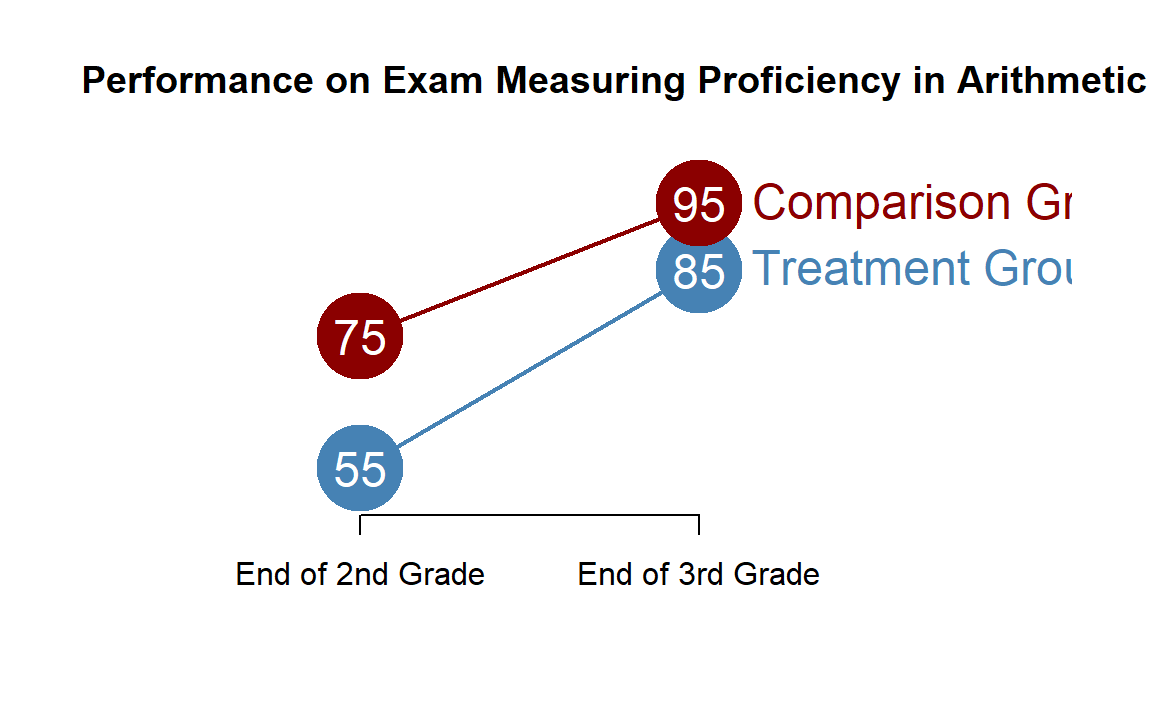
\includegraphics[width=0.7\linewidth]{Foundations_of_Program_Evaluation_files/figure-latex/unnamed-chunk-24-1} \end{center}

\hypertarget{gains-realized-by-comparison-group-the-first-difference}{%
\subsection{Gains Realized by Comparison Group (The First
Difference)}\label{gains-realized-by-comparison-group-the-first-difference}}

As we try to measure the impact of a specific program we have to keep in
mind that other factors may influence outcomes over time. These are
often referred to as secular trends, or changes that we expect to see
independent of the intervention.

\[ \textrm{Trend} = C2 - C1 = 95 - 75 = 20 \]

\hypertarget{gains-realized-by-the-treatment-group-the-second-difference}{%
\subsection{Gains Realized by the Treatment Group (The Second
Difference)}\label{gains-realized-by-the-treatment-group-the-second-difference}}

If we want to determine program impact we can measure the change in the
treatment group based upon our outcome level before receiving the
treatment and after receiving the treatment. This shows total change
over the treatment period. It will also contain both changes
attributable to program impact, as well as general changes attributable
to trend.

\[ \textrm{Treatment Group Gains} = T2 - T1 = 85 - 55 = 30\]

\hypertarget{realized-gains-minus-expected-gains-diff-in-diff}{%
\subsection{Realized Gains Minus Expected Gains
(Diff-in-Diff)}\label{realized-gains-minus-expected-gains-diff-in-diff}}

In order to isolate program impacts we must subtract out the gains that
we would expect the treatment group to make independent of the program.
The total gain minus the gain from trend is called the
difference-in-difference estimate.

\[ \textrm{Treatment Gains - Trend} = (T2 - T1) - (C2 - C1) = 30 - 20 = 10 \]
In this case we can see that the tutoring program is leading to gains of
an extra ten points more than what we would expect from a typical third
grader over the year not enrolled in the program.

\hypertarget{the-counterfactual}{%
\section{The Counterfactual}\label{the-counterfactual}}

Any time we measure the impact of a program we must compare the final
state of the treatment group to some other state of the world. The
sensible question is to ask, what would this group look like if it had
not received the treatment?

\begin{quote}
The counterfactual tells us what the treatment group would look like if
there was no program impact.
\end{quote}

If we have the luxury of performing a randomized experiment then from
the statistical standpoint the control group embodies the
counterfactual. If randomized is done successfully the only difference
between the treatment and control group will be, on average, whether the
members received the treatment or not. This simplifies our lives because
after the study we can attibute all of the differences in group means to
the program effects.

\begin{center}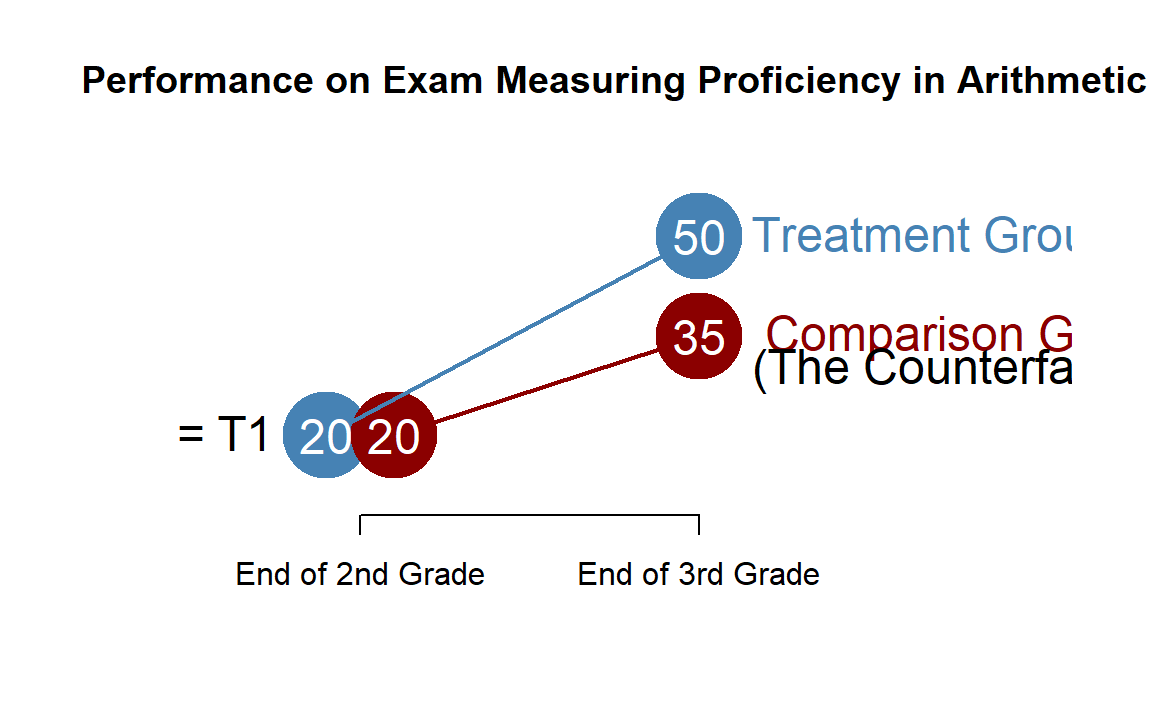
\includegraphics[width=0.7\linewidth]{Foundations_of_Program_Evaluation_files/figure-latex/unnamed-chunk-25-1} \end{center}

In most cases, however, we do not have the opportunity or ability to
conduct a true experiment. Instead, we need to create a reasonable
comparision group that we can use for counterfactual analysis, and we
can use this group to observe changes we expect to see indepedent of the
treatment. This is the first difference, or the trend in the example
above.

Since our treatment group and our comparison group might not have
identical pre-treatment characteristics the counterfactual must account
for these differences. The proper way to think about this is:

\[ \textrm{Counterfactual} = T1 + Trend \]

\begin{center}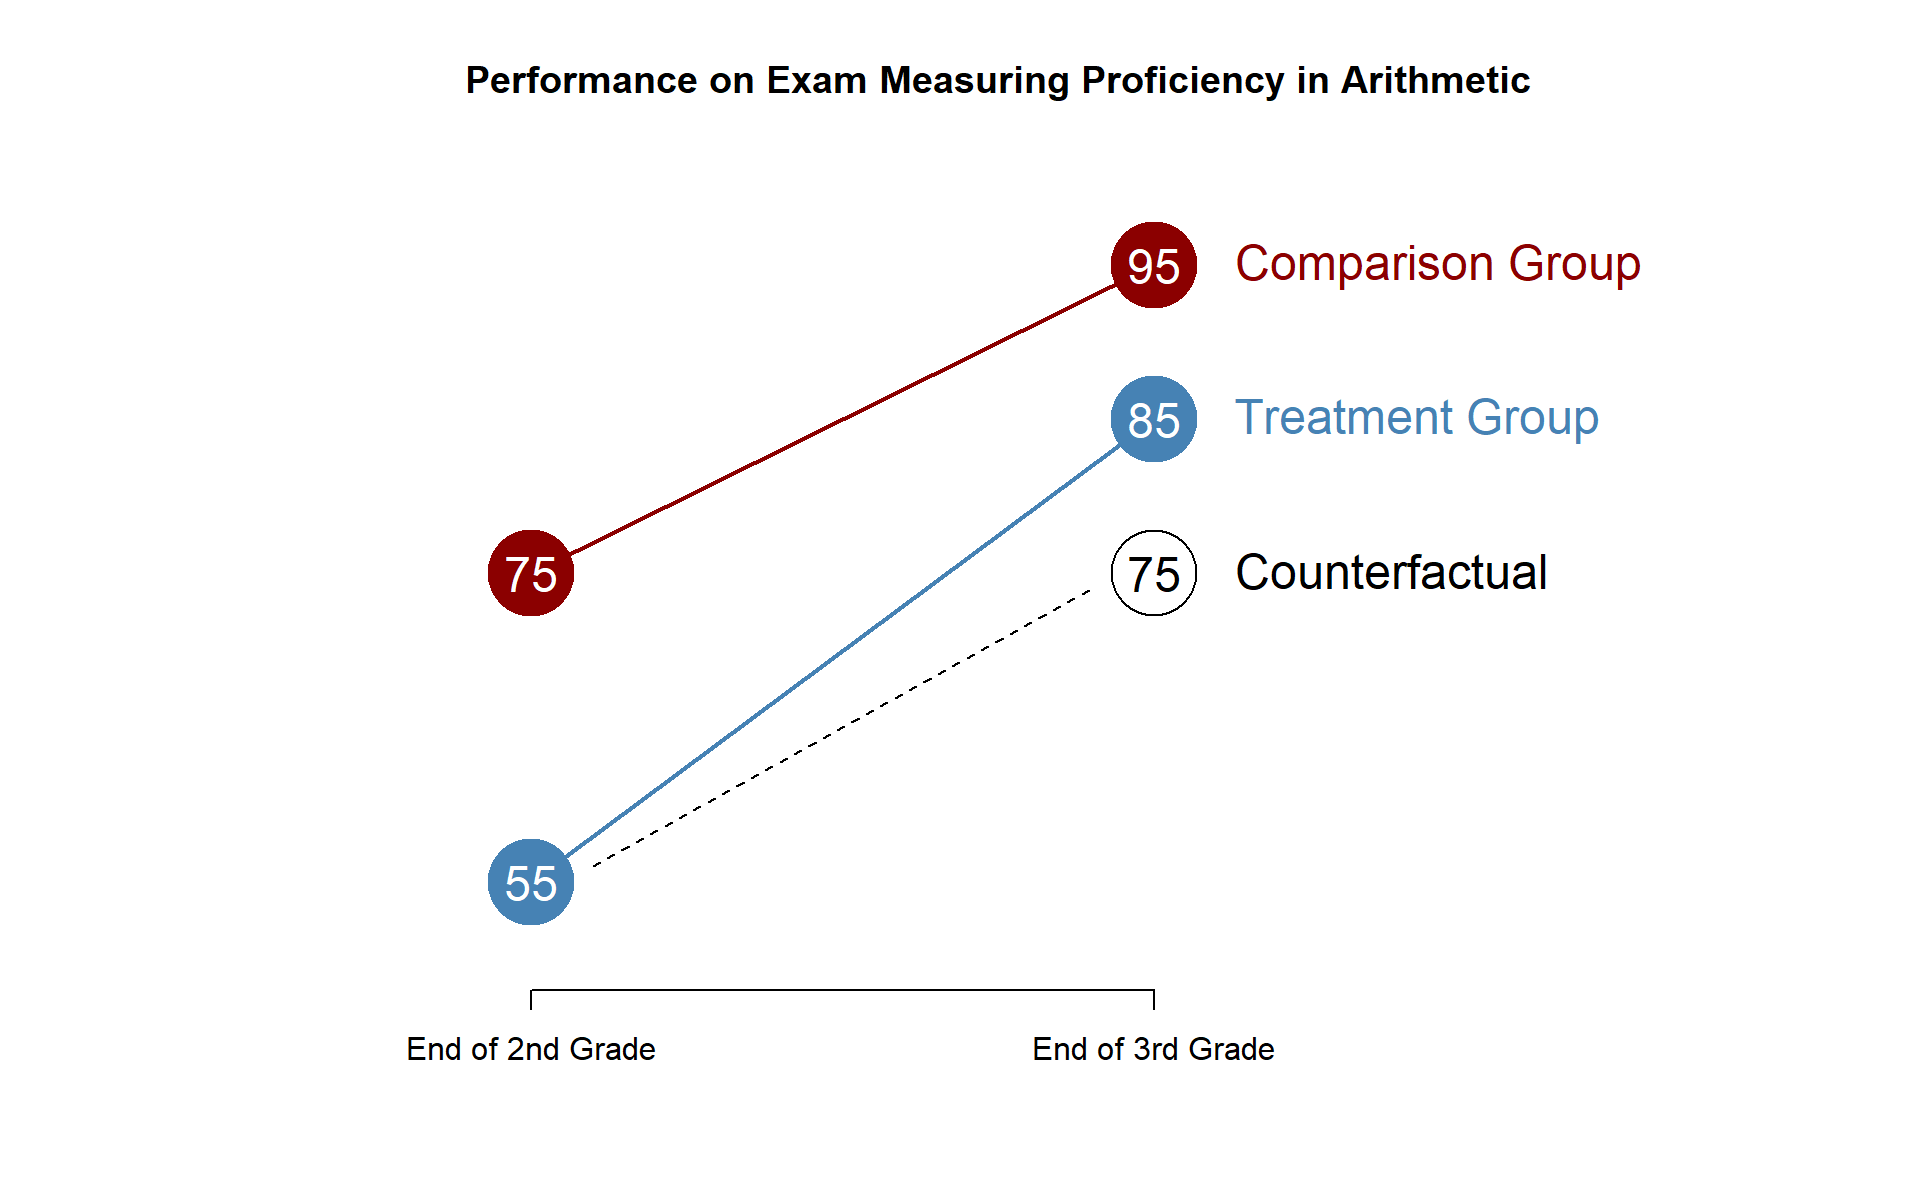
\includegraphics[width=0.7\linewidth]{Foundations_of_Program_Evaluation_files/figure-latex/unnamed-chunk-26-1} \end{center}

Any time we calculate a program treatment effect there is an explicit or
an implied counterfactual. The problematic evaluations are usually ones
in which they are unclear about the counterfactual in the study.

\hypertarget{difference-in-difference-models-1}{%
\section{Difference-in-Difference
Models}\label{difference-in-difference-models-1}}

The formal difference-in-difference estimate uses a regression model to
examine program effects. It is a slightly odd regression because all of
the variables in the model are dummy variables. The model is written as
follows:

\[ Y = b_{0} + b_{1} \cdot Treat + b_{2} \cdot Post + b_{3} \cdot Treat \cdot Post + e \]

The data looks something like this:

\begin{tabular}{l|l|l|l|l}
\hline
y & intercept & treat & post & treat\_post\\
\hline
y1 & 1 & 0 & 0 & 0\\
\hline
y2 & 1 & 0 & 1 & 0\\
\hline
y3 & 1 & 1 & 0 & 0\\
\hline
y4 & 1 & 1 & 1 & 1\\
\hline
 & A & B & C & D\\
\hline
\end{tabular}

In this example, y1 to y4 represent some measured level of the outcome.
The intercept in the model is a vector of all 1's. And each other
variable is a dummy variable. Note that the last term in this model,
\emph{treat\_post} is an interaction effect. It is created by
multiplying the variables \emph{treat} and \emph{post}.

\hypertarget{example-1}{%
\subsection{Example}\label{example-1}}

Let's consider the following case:

\begin{center}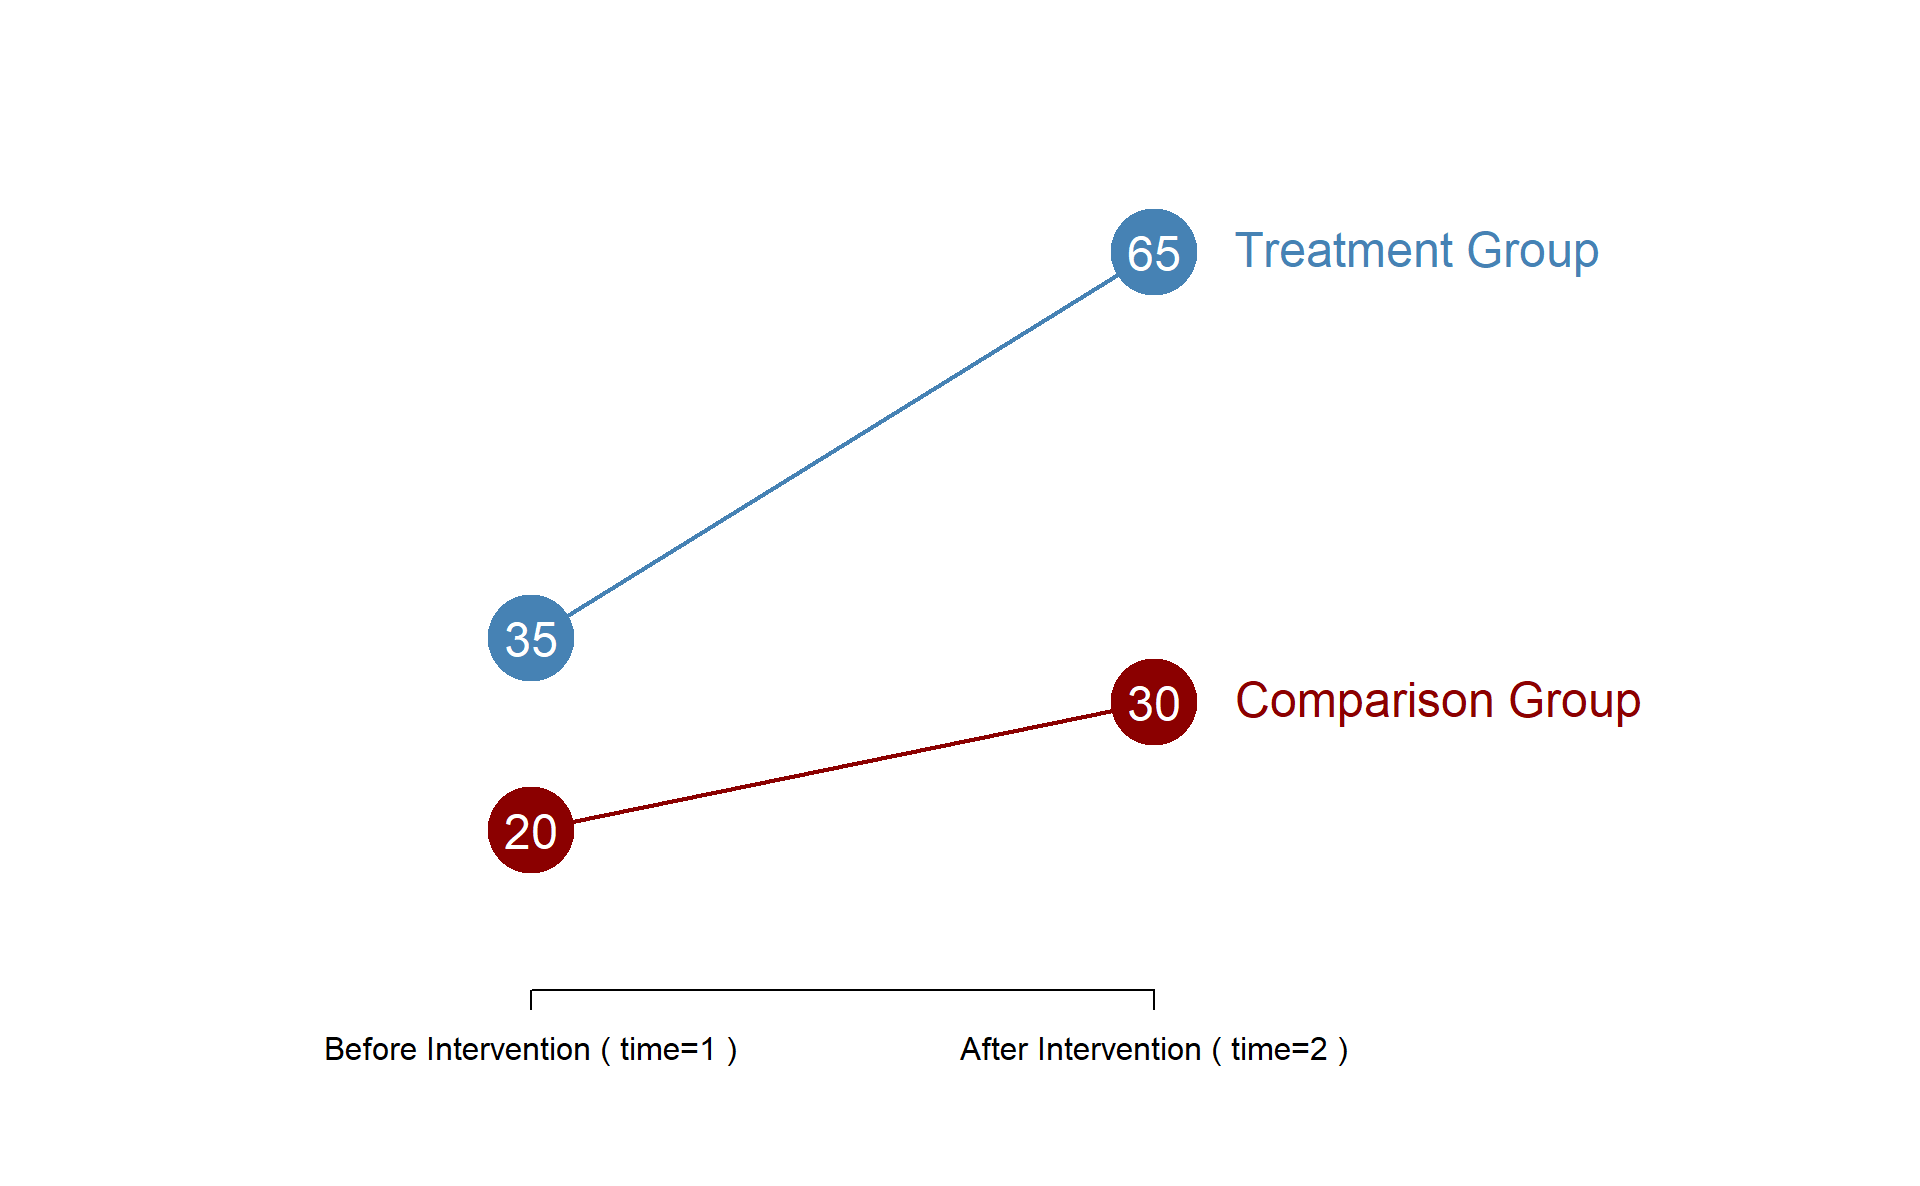
\includegraphics[width=0.7\linewidth]{Foundations_of_Program_Evaluation_files/figure-latex/unnamed-chunk-28-1} \end{center}

Now let us estimate this model using our difference-in-difference
regression, which gives us the following results:

\begin{tabular}{r|r|r}
\hline
moxy & treat & post\\
\hline
20 & 0 & 0\\
\hline
20 & 0 & 0\\
\hline
20 & 0 & 0\\
\hline
20 & 0 & 0\\
\hline
20 & 0 & 0\\
\hline
20 & 0 & 0\\
\hline
\end{tabular}

\begin{Shaded}
\begin{Highlighting}[]

\NormalTok{m0 <-}\StringTok{ }\KeywordTok{lm}\NormalTok{( moxy }\OperatorTok{~}\StringTok{ }\NormalTok{C1 }\OperatorTok{+}\StringTok{ }\NormalTok{C2 }\OperatorTok{+}\StringTok{ }\NormalTok{T1 }\OperatorTok{+}\StringTok{ }\NormalTok{T2 }\OperatorTok{-}\StringTok{ }\DecValTok{1}\NormalTok{ )}

\NormalTok{m1 <-}\StringTok{ }\KeywordTok{lm}\NormalTok{( moxy }\OperatorTok{~}\StringTok{ }\NormalTok{treat )}

\NormalTok{m2 <-}\StringTok{ }\KeywordTok{lm}\NormalTok{( moxy }\OperatorTok{~}\StringTok{ }\NormalTok{post )}

\NormalTok{m3 <-}\StringTok{ }\KeywordTok{lm}\NormalTok{( moxy }\OperatorTok{~}\StringTok{ }\NormalTok{treat }\OperatorTok{+}\StringTok{ }\NormalTok{post )}

\NormalTok{m4 <-}\StringTok{ }\KeywordTok{lm}\NormalTok{( moxy }\OperatorTok{~}\StringTok{ }\NormalTok{treat }\OperatorTok{+}\StringTok{ }\NormalTok{post }\OperatorTok{+}\StringTok{ }\NormalTok{treat}\OperatorTok{*}\NormalTok{post )}

\CommentTok{# library( stargazer )}

\KeywordTok{stargazer}\NormalTok{( m4, }\DataTypeTok{type=}\StringTok{'html'}\NormalTok{, }\DataTypeTok{digits=}\DecValTok{0}\NormalTok{,}
           \DataTypeTok{omit.stat=}\KeywordTok{c}\NormalTok{(}\StringTok{"f"}\NormalTok{,}\StringTok{"rsq"}\NormalTok{,}\StringTok{"adj.rsq"}\NormalTok{,}\StringTok{"ser"}\NormalTok{),}
           \DataTypeTok{intercept.bottom =} \OtherTok{FALSE}\NormalTok{,}
           \DataTypeTok{covariate.labels =} \KeywordTok{c}\NormalTok{(}\StringTok{"b0: Intercept (A)"}\NormalTok{, }\StringTok{"b1: Treatment Group (B)"}\NormalTok{,}
                                \StringTok{"b2: Post-Period (C)"}\NormalTok{, }\StringTok{"b3: Treat x Post (D)"}\NormalTok{ ) )}
\end{Highlighting}
\end{Shaded}

Dependent variable:

moxy

b0: Intercept (A)

20***

(0)

b1: Treatment Group (B)

15***

(0)

b2: Post-Period (C)

10***

(0)

b3: Treat x Post (D)

20***

(0)

Observations

400

Note:

\emph{p\textless{}0.1; \textbf{p\textless{}0.05; }}p\textless{}0.01

It takes a little bit of knowledge to make sense of the results. The
important insight is that each coefficient represents a component of the
outcome, so you need to add components together to get the actual group
means.

The other important insight is that each coefficient represents a
distinctive statistical test.

Recall that we can conduct a t-test using a regression model by
including a dummy variable. The coefficient in the regression model will
represent the group mean difference, and the significance level will be
identical to a normal t-test.

When you test a difference in means between two groups it is called a
contrast. Since we have multiple dummy variables in our model we have
multiple contrasts. To understand each test you must understand the
implied reference group of each test.

\begin{center}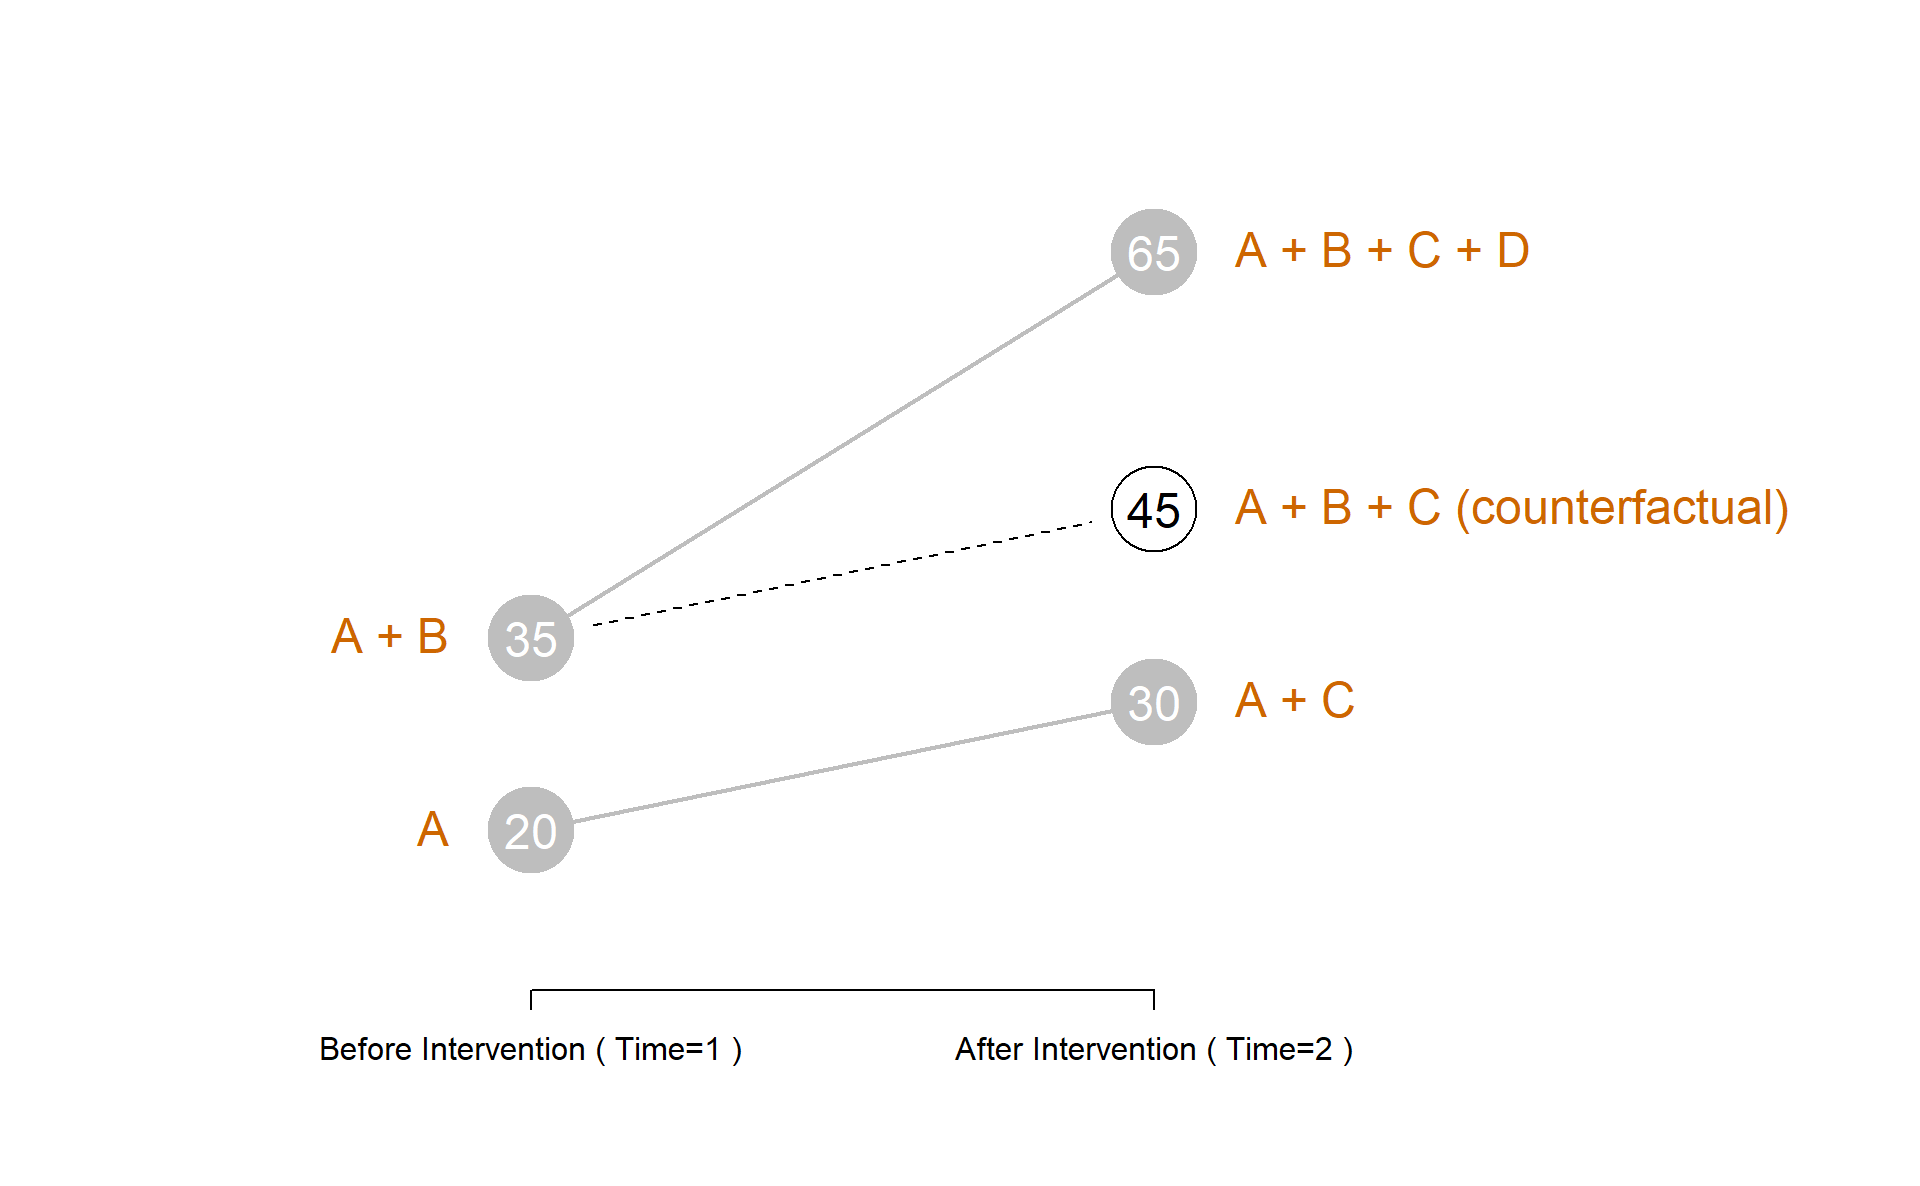
\includegraphics[width=0.7\linewidth]{Foundations_of_Program_Evaluation_files/figure-latex/unnamed-chunk-31-1} \end{center}

\hypertarget{interpretation}{%
\subsection{Interpretation}\label{interpretation}}

For example, the Comparison Group during the first period of the study
has a mean outcome of 20. Since we have included a dummy variable
representing our Treatment Group in the model, the omitted category is
the Comparison Group, so it ends up in the intercept \(b_{0}\) in our
regression model. Similarly, since we have a dummy variable representing
the Post-Intervention time period, the omitted category is
Pre-Intervention, which also defaults to the intercept. A on the diagram
above then represents the non-Treatment, non-Post Intervention group, or
the Comparison Group in the Pre-Intervention period.

Similar to other regression models, each coefficient has an associated
level of significance. Similar to other regressions we have run, this
level of significance represents a hypothesis test of whether the
coefficient is equal to zero. In the typical case with a continuous
numerical measure, if the slope is equal to zero it represents no
relationship. In this case it is a t-test of whether the mean of the
base group is equal to zero.

The Comparison Group during the second time period has a mean outcome of
30. We don't have a coefficient for Comparison Group Time=2 specifically
in our model, so we must construct the group mean from other
coefficients. We can see that the group can be represented by adding up
A + C on the diagram, or adding the coefficient \(b_{2}\) to the
intercept (10 + 20) to arrive at the group mean of 30.

Similarly, we can find the group mean for the Treatment Group at Time=1
by adding the coefficient \(b_{1}\) to the base group, 20 + 15, to get
35. This is represented by A + B in the diagram above.

Let's pause for a moment and consider the statistical significant
associated with coefficients \(b_{1}\) and \(b_{2}\). Here is where the
reference group becomes important. Since each coefficient represents the
difference between the group mean and the reference group, the
hypothesis is a test of whether the outcome in those groups differ.

Since \(b_{1}\) is 15, the coefficient represents a test of whether
\(T1 - C1 = 0\). In other words, did the Treatment and Comparison groups
differ significantly in the first time period?

Since \(b_{2}\) is 10, the coefficient represents a test of whether
\(C2 - C1 = 0\). In other words, did the Comparison group change
significantly between the first and second time periods?

Now the last contrast is the tricky one. To make sense of this one we
need to think about the reference group for this contrast. Note that we
can create a Post-Test Treatment group by adding
\(b_{0} + b_{1} + b_{2}\) (A + B + C on the diagram), but this only
comes to 20 + 10 + 15, or 45. The actual mean outcome measured for group
T2 is 65. So how do we arrive at this number?

Recall that \(b_{3}\) represents the coefficient from an
\emph{interaction} effect. The interpretation is an interaction is that
the whole is greater than the sum of the parts. When an interaction is
present, we observe an impact larger than the impact of two independent
direct effects (the gains from being in the Treatment group, and the
expected gains from the secular trend, in this case).

The measure \(b_{0} + b_{1} + b_{2}\) tells us where we should expect
the group mean of T2 to reside (the counterfactual), and the coefficient
\(b_{3}\) tells us whether the actual group mean is different,
i.e.~whether we experiences a treatment effect from this program. We see
in the model that \(b_{3}=20\), meaning the observed group mean is 20
points higher than we would expect if the treatment did not work.

\hypertarget{summary-of-hypothesis-tested}{%
\subsection{Summary of Hypothesis
Tested}\label{summary-of-hypothesis-tested}}

Is the Comparison Group in Time=1 different from zero?

\begin{itemize}
\tightlist
\item
  Coefficient \(b_{0}\)
\item
  \(Null: C1 = 0\)
\end{itemize}

Is the Treatment Group different from the Comparison Group in Time=1?

\begin{itemize}
\tightlist
\item
  Coefficient \(b_{1}\)
\item
  \(Null: T1 - C1 = 0\)
\end{itemize}

Is the Comparision Group in Time=2 different than the Comparison Group
in Time=1? I.e. is there a secular trend?

\begin{itemize}
\tightlist
\item
  Coefficient \(b_{2}\)
\item
  \(Null: C2 - C1 = 0\)
\end{itemize}

Is the Treatment Group in Time=2 different from the counterfactual? Does
the program have impact?

\begin{itemize}
\tightlist
\item
  Coefficient \(b_{3}\)
\item
  \(Null: (T2-T1) - (C2-C1) = 0\)
\end{itemize}

\hypertarget{three-cases}{%
\subsection{Three Cases}\label{three-cases}}

Let us consider three cases where statistical significance might be of
interest.

\begin{center}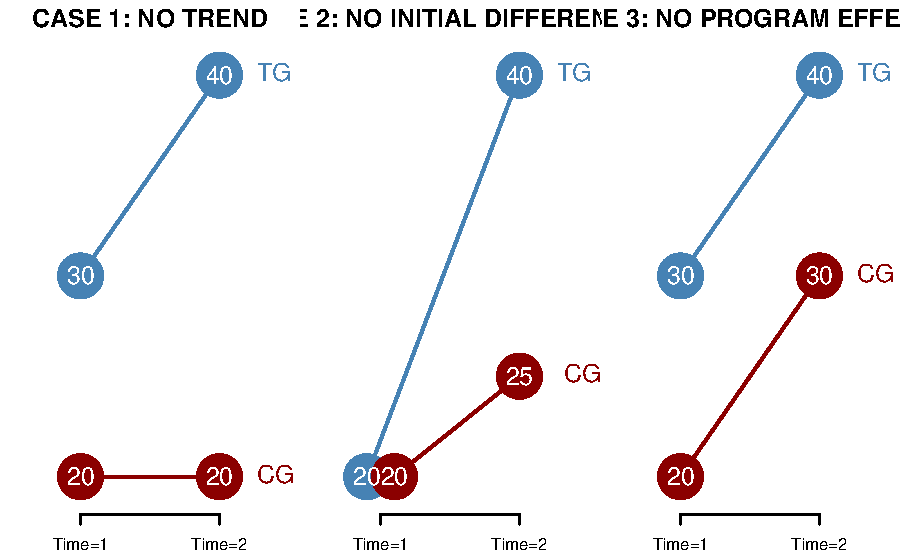
\includegraphics[width=0.7\linewidth]{Foundations_of_Program_Evaluation_files/figure-latex/unnamed-chunk-32-1} \end{center}

The regression results would be as follows:

\begin{Shaded}
\begin{Highlighting}[]


\CommentTok{# m1 <- lm( moxy ~ treat + post + treat*post )}
\CommentTok{# m2 <- lm( moxy ~ treat + post + treat*post )}
\CommentTok{# m3 <- lm( moxy ~ treat + post + treat*post )}



\KeywordTok{stargazer}\NormalTok{( m1, m2, m3, }\DataTypeTok{type=}\StringTok{'html'}\NormalTok{, }\DataTypeTok{digits=}\DecValTok{1}\NormalTok{,}
           \DataTypeTok{omit.stat=}\KeywordTok{c}\NormalTok{(}\StringTok{"f"}\NormalTok{,}\StringTok{"rsq"}\NormalTok{,}\StringTok{"adj.rsq"}\NormalTok{,}\StringTok{"ser"}\NormalTok{),}
           \DataTypeTok{intercept.bottom =} \OtherTok{FALSE}\NormalTok{,}
           \DataTypeTok{covariate.labels =} \KeywordTok{c}\NormalTok{(}\StringTok{"Intercept (A)"}\NormalTok{, }\StringTok{"Treatment Group (B)"}\NormalTok{,}
                                \StringTok{"Post-Period (C)"}\NormalTok{, }\StringTok{"Treat x Post (D)"}\NormalTok{ ) )}
\end{Highlighting}
\end{Shaded}

Dependent variable:

moxy

(1)

(2)

(3)

Intercept (A)

20.0***

20.0***

20.0***

(1.4)

(1.4)

(1.4)

Treatment Group (B)

10.0***

-0.0

10.0***

(1.9)

(1.9)

(1.9)

Post-Period (C)

-0.0

5.0**

10.0***

(1.9)

(1.9)

(1.9)

Treat x Post (D)

10.0***

15.0***

0.0

(2.7)

(2.7)

(2.7)

Observations

84

84

84

Note:

\emph{p\textless{}0.1; \textbf{p\textless{}0.05; }}p\textless{}0.01

Note the lack of significance for the specific hypotheses in each case.

Case 1: When \(b_{2}\) is not significant, it tells us there is no
secular trend in the data.

Case 2: When \(b_{1}\) is not significant, it tells us there is no
different between the measured outcomes of the treatment and comparison
groups during the first time period.

Case 3: When \(b_{3}\) is not significant, it tells us that all gains
observed in the treatment group are coming from the secular trend and
not the program.

\hypertarget{multiple-treatment-groups}{%
\subsection{Multiple Treatment Groups}\label{multiple-treatment-groups}}

Sometimes your study may contain multiple treatment groups.

\begin{center}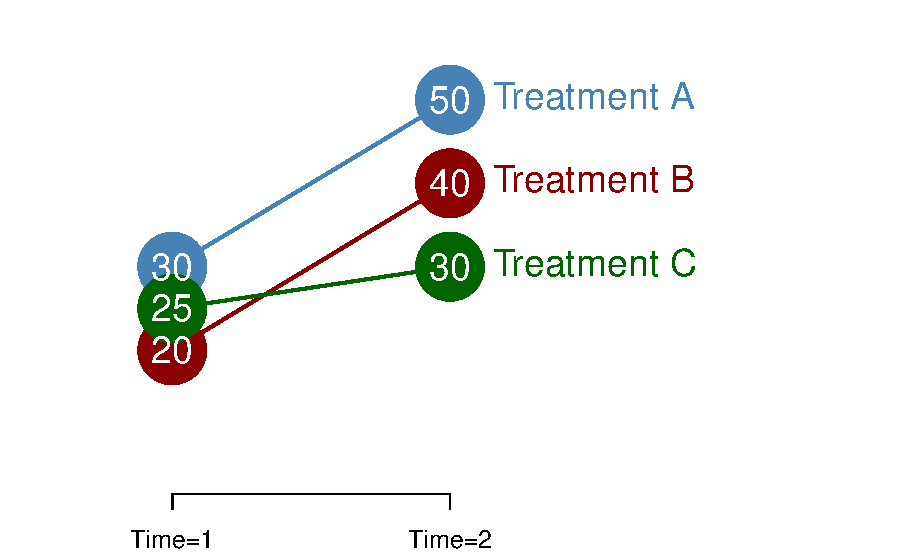
\includegraphics[width=0.7\linewidth]{Foundations_of_Program_Evaluation_files/figure-latex/unnamed-chunk-35-1} \end{center}

In order to specify the regression we again must omit one group, which
will become the reference group in the study. In this case we will omit
Treatement C as the reference group.

\begin{Shaded}
\begin{Highlighting}[]

      
\NormalTok{A1 <-}\StringTok{ }\KeywordTok{seq}\NormalTok{(}\DecValTok{20}\NormalTok{,}\DecValTok{40}\NormalTok{)}
\NormalTok{A2 <-}\StringTok{ }\KeywordTok{seq}\NormalTok{(}\DecValTok{40}\NormalTok{,}\DecValTok{60}\NormalTok{)}
\NormalTok{B1 <-}\StringTok{ }\KeywordTok{seq}\NormalTok{(}\DecValTok{10}\NormalTok{,}\DecValTok{30}\NormalTok{)}
\NormalTok{B2 <-}\StringTok{ }\KeywordTok{seq}\NormalTok{(}\DecValTok{30}\NormalTok{,}\DecValTok{50}\NormalTok{)}
\NormalTok{C1 <-}\StringTok{ }\KeywordTok{seq}\NormalTok{(}\DecValTok{15}\NormalTok{,}\DecValTok{35}\NormalTok{)}
\NormalTok{C2 <-}\StringTok{ }\KeywordTok{seq}\NormalTok{(}\DecValTok{20}\NormalTok{,}\DecValTok{40}\NormalTok{)}


\NormalTok{moxy <-}\StringTok{ }\KeywordTok{c}\NormalTok{(A1,A2,B1,B2,C1,C2)}
\NormalTok{GroupA <-}\StringTok{ }\KeywordTok{rep}\NormalTok{( }\KeywordTok{c}\NormalTok{(}\DecValTok{1}\NormalTok{,}\DecValTok{0}\NormalTok{,}\DecValTok{0}\NormalTok{), }\DataTypeTok{each=}\DecValTok{42}\NormalTok{ )}
\NormalTok{GroupB <-}\StringTok{ }\KeywordTok{rep}\NormalTok{( }\KeywordTok{c}\NormalTok{(}\DecValTok{0}\NormalTok{,}\DecValTok{1}\NormalTok{,}\DecValTok{0}\NormalTok{), }\DataTypeTok{each=}\DecValTok{42}\NormalTok{ )}
\NormalTok{GroupC <-}\StringTok{ }\KeywordTok{rep}\NormalTok{( }\KeywordTok{c}\NormalTok{(}\DecValTok{0}\NormalTok{,}\DecValTok{0}\NormalTok{,}\DecValTok{1}\NormalTok{), }\DataTypeTok{each=}\DecValTok{42}\NormalTok{ )}
\NormalTok{post <-}\StringTok{ }\KeywordTok{rep}\NormalTok{( }\KeywordTok{c}\NormalTok{(}\DecValTok{0}\NormalTok{,}\DecValTok{1}\NormalTok{,}\DecValTok{0}\NormalTok{,}\DecValTok{1}\NormalTok{,}\DecValTok{0}\NormalTok{,}\DecValTok{1}\NormalTok{), }\DataTypeTok{each=}\DecValTok{21}\NormalTok{ )}


\NormalTok{m1 <-}\StringTok{ }\KeywordTok{lm}\NormalTok{( moxy }\OperatorTok{~}\StringTok{ }\NormalTok{post }\OperatorTok{+}\StringTok{ }\NormalTok{GroupA }\OperatorTok{+}\StringTok{ }\NormalTok{GroupB  }\OperatorTok{+}\StringTok{ }\NormalTok{GroupA}\OperatorTok{*}\NormalTok{post }\OperatorTok{+}\StringTok{ }\NormalTok{GroupB}\OperatorTok{*}\NormalTok{post )}



\KeywordTok{stargazer}\NormalTok{( m1, }\DataTypeTok{type=}\StringTok{'html'}\NormalTok{, }\DataTypeTok{digits=}\DecValTok{1}\NormalTok{,}
           \DataTypeTok{omit.stat=}\KeywordTok{c}\NormalTok{(}\StringTok{"f"}\NormalTok{,}\StringTok{"rsq"}\NormalTok{,}\StringTok{"adj.rsq"}\NormalTok{,}\StringTok{"ser"}\NormalTok{),}
           \DataTypeTok{intercept.bottom =} \OtherTok{FALSE}\NormalTok{,}
           \DataTypeTok{covariate.labels =} \KeywordTok{c}\NormalTok{(}\StringTok{"b0: Intercept"}\NormalTok{, }\StringTok{"b1: Post"}\NormalTok{,}\StringTok{"b2: Treatment A"}\NormalTok{,}
                                \StringTok{"b3: Treatment B"}\NormalTok{, }\StringTok{"b4: A x Post"}\NormalTok{, }\StringTok{"b5: B x Post"}\NormalTok{ ) )}
\end{Highlighting}
\end{Shaded}

Dependent variable:

moxy

b0: Intercept

25.0***

(1.4)

b1: Post

5.0**

(1.9)

b2: Treatment A

5.0**

(1.9)

b3: Treatment B

-5.0**

(1.9)

b4: A x Post

15.0***

(2.7)

b5: B x Post

15.0***

(2.7)

Observations

126

Note:

\emph{p\textless{}0.1; \textbf{p\textless{}0.05; }}p\textless{}0.01

Note that you will again build group means from their component parts.
For example, Treatment A can be represented as \(b_{0} + b_{2}\) in
period one, and \(b_{0} + b_{1} + b_{2} + b_{4}\) for period two.

The main thing to note is that the counterfactual has now become the
gains that you expect in the omitted group. It makes sense in this case
to omit the group with the least gains because then you can interpret
the program effects \(b_{3}\) or \(b_{4}\) as gains you expect over the
least effective treatment option.

Note that the coefficient \(b_{1}\) associated with the Post-Treatment
period is no longer interpretted as trend.

\hypertarget{interactions-with-slopes}{%
\chapter{Interactions with Slopes}\label{interactions-with-slopes}}

The difference-in-difference model can be extended to circumstances
where we have multiple treatments, but instead of moving from only two
scenarios of no treatment (time=1) to treatment (time=2), we move from
low levels of treatment to high levels of treatment. In other words, our
treatment represents a continuous variable, not a binary one, and we are
back in the world of regression slopes.

We can adapt our difference-in-difference framework to accomodate these
types of interaction models as well. Let's consider an example where we
have developed three types of hybrid corns and we are trying to
understand how these new varieties will respond to our fertilizer.

\begin{tabular}{r|r|l|r|r|r}
\hline
height & fertilizer & type & dumA & dumB & dumC\\
\hline
84.88238 & 1 & A & 1 & 0 & 0\\
\hline
81.58291 & 2 & A & 1 & 0 & 0\\
\hline
83.43583 & 3 & A & 1 & 0 & 0\\
\hline
68.82138 & 4 & A & 1 & 0 & 0\\
\hline
80.85738 & 5 & A & 1 & 0 & 0\\
\hline
81.04858 & 6 & A & 1 & 0 & 0\\
\hline
\end{tabular}

\hypertarget{one-slope---one-intercept-model}{%
\section{One Slope - One Intercept
Model}\label{one-slope---one-intercept-model}}

Let's start with a basic model and build up to a more complicated model.
We can first test whether the fertilizer has any impact on corn growth,
ignoring the different types of hybrids for now:

\begin{Shaded}
\begin{Highlighting}[]


\KeywordTok{plot}\NormalTok{( fertilizer, height, }\DataTypeTok{col=}\KeywordTok{gray}\NormalTok{(}\FloatTok{0.5}\NormalTok{,}\FloatTok{0.5}\NormalTok{), }\DataTypeTok{bty=}\StringTok{"n"}\NormalTok{, }\DataTypeTok{cex=}\DecValTok{2}\NormalTok{, }\DataTypeTok{pch=}\DecValTok{19}\NormalTok{,}
      \DataTypeTok{xlab=}\StringTok{"Fertilizer Intensity"}\NormalTok{, }\DataTypeTok{ylab=}\StringTok{"Height of Corn"}\NormalTok{, }
      \DataTypeTok{main=}\StringTok{"Effect of Fertilizer on Corn Growth: Three Hybrid Types"}\NormalTok{)}

\KeywordTok{abline}\NormalTok{( }\KeywordTok{lm}\NormalTok{( height }\OperatorTok{~}\StringTok{ }\NormalTok{fertilizer ), }\DataTypeTok{col=}\StringTok{"darkred"}\NormalTok{, }\DataTypeTok{lwd=}\DecValTok{2}\NormalTok{ )}
\end{Highlighting}
\end{Shaded}

\begin{center}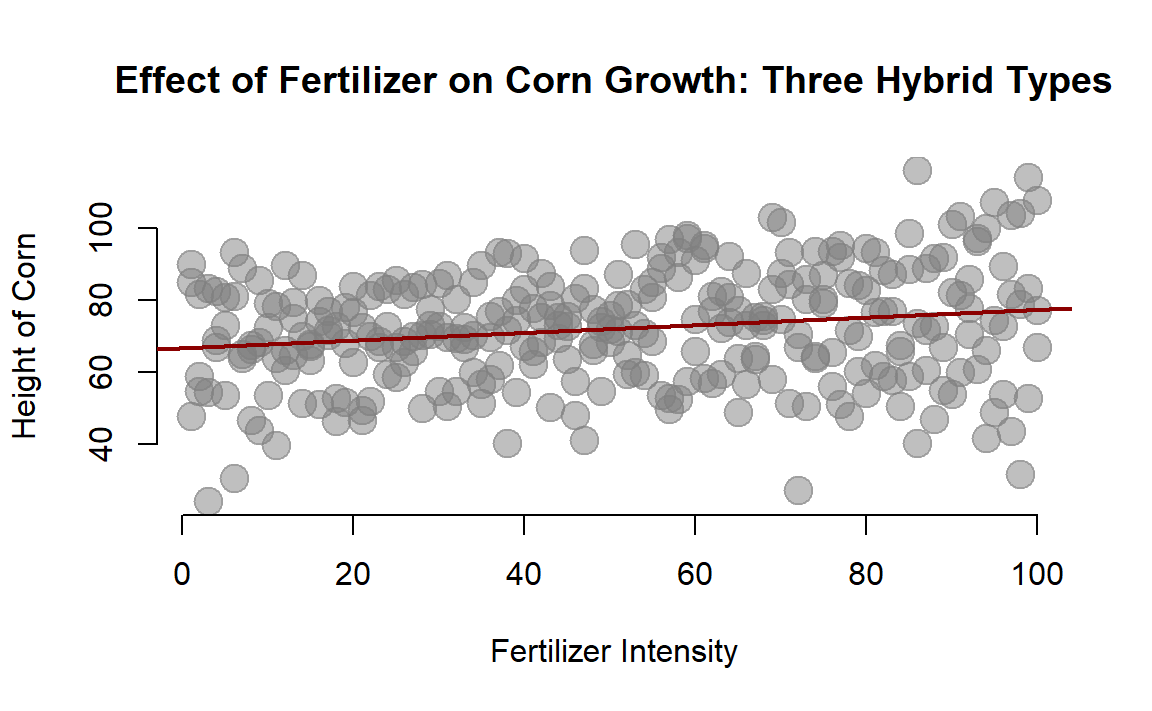
\includegraphics[width=0.7\linewidth]{Foundations_of_Program_Evaluation_files/figure-latex/unnamed-chunk-38-1} \end{center}

We can see that we have a positive slope, which is statistically
significant. So our fertilize does seem to have a positive effect on the
corn.

\begin{Shaded}
\begin{Highlighting}[]


\NormalTok{m}\FloatTok{.00}\NormalTok{ <-}\StringTok{ }\KeywordTok{lm}\NormalTok{( height }\OperatorTok{~}\StringTok{ }\NormalTok{fertilizer )}


\KeywordTok{stargazer}\NormalTok{( m}\FloatTok{.00}\NormalTok{, }\DataTypeTok{type=}\StringTok{"html"}\NormalTok{, }
           \DataTypeTok{digits=}\DecValTok{2}\NormalTok{, }\DataTypeTok{omit.stat =} \KeywordTok{c}\NormalTok{(}\StringTok{"ser"}\NormalTok{) )}
\end{Highlighting}
\end{Shaded}

Dependent variable:

height

fertilizer

0.11***

(0.03)

Constant

66.77***

(1.80)

Observations

300

R2

0.04

Adjusted R2

0.04

F Statistic

11.97*** (df = 1; 298)

Note:

\emph{p\textless{}0.1; \textbf{p\textless{}0.05; }}p\textless{}0.01

\hypertarget{three-types-of-hybrids}{%
\section{Three Types of Hybrids}\label{three-types-of-hybrids}}

Let's now consider the strength of each type of hybrid.

\begin{Shaded}
\begin{Highlighting}[]


\KeywordTok{palette}\NormalTok{( }\KeywordTok{c}\NormalTok{( }\KeywordTok{adjustcolor}\NormalTok{( }\StringTok{"forestgreen"}\NormalTok{, }\DataTypeTok{alpha.f=}\FloatTok{0.5}\NormalTok{), }
            \KeywordTok{adjustcolor}\NormalTok{( }\StringTok{"darkorange3"}\NormalTok{, }\DataTypeTok{alpha.f=}\FloatTok{0.5}\NormalTok{),}
            \KeywordTok{adjustcolor}\NormalTok{( }\StringTok{"darkmagenta"}\NormalTok{, }\DataTypeTok{alpha.f=}\FloatTok{0.5}\NormalTok{) ) )}
            
\KeywordTok{plot}\NormalTok{( fertilizer, height, }\DataTypeTok{col=}\KeywordTok{factor}\NormalTok{(type), }\DataTypeTok{pch=}\DecValTok{19}\NormalTok{, }\DataTypeTok{bty=}\StringTok{"n"}\NormalTok{, }\DataTypeTok{cex=}\DecValTok{2}\NormalTok{,}
      \DataTypeTok{xlab=}\StringTok{"Fertilizer Intensity"}\NormalTok{, }\DataTypeTok{ylab=}\StringTok{"Height of Corn"}\NormalTok{, }
      \DataTypeTok{main=}\StringTok{"Effect of Fertilizer on Corn Growth: Three Hybrid Types"}\NormalTok{)}
\end{Highlighting}
\end{Shaded}

\begin{center}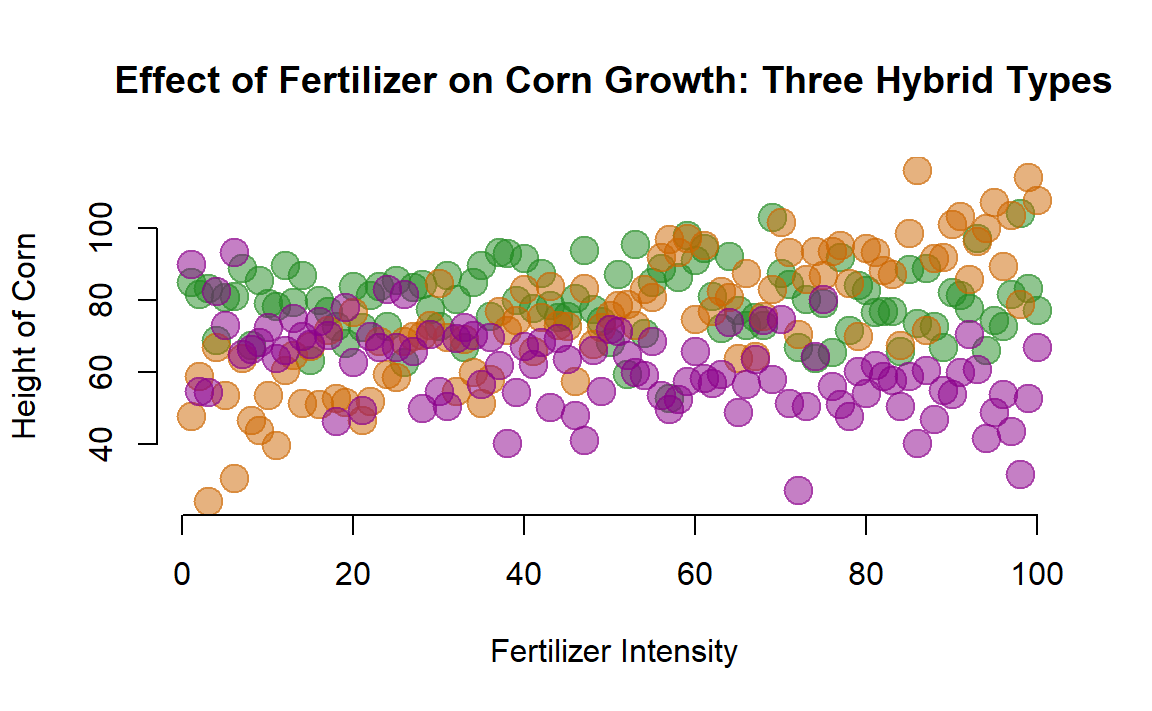
\includegraphics[width=0.7\linewidth]{Foundations_of_Program_Evaluation_files/figure-latex/unnamed-chunk-40-1} \end{center}

\hypertarget{one-slope---three-intercepts}{%
\section{One Slope - Three
Intercepts}\label{one-slope---three-intercepts}}

Let's extend our original model slightly by still examinig the impact of
fertilizer on corn height, but let's allow each variety to have its own
intercept term. We can do this by adding a dummy variable for each
hybrid type.

\begin{center}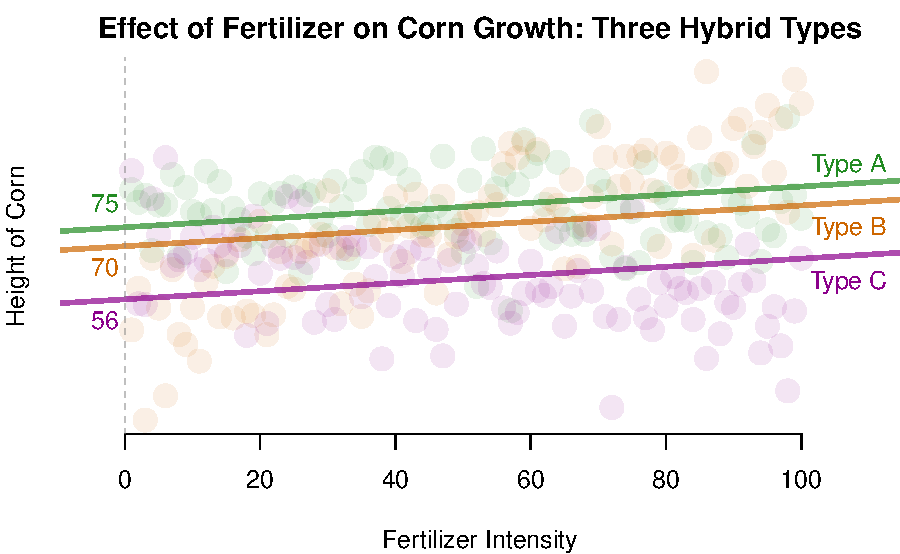
\includegraphics[width=0.7\linewidth]{Foundations_of_Program_Evaluation_files/figure-latex/unnamed-chunk-41-1} \end{center}

\begin{Shaded}
\begin{Highlighting}[]


\KeywordTok{stargazer}\NormalTok{( m}\FloatTok{.01}\NormalTok{, m}\FloatTok{.02}\NormalTok{, m}\FloatTok{.03}\NormalTok{, m}\FloatTok{.04}\NormalTok{, }\DataTypeTok{type=}\StringTok{"html"}\NormalTok{, }
           \DataTypeTok{digits=}\DecValTok{2}\NormalTok{, }
          \DataTypeTok{omit.stat=}\KeywordTok{c}\NormalTok{(}\StringTok{"f"}\NormalTok{,}\StringTok{"adj.rsq"}\NormalTok{,}\StringTok{"ser"}\NormalTok{),}
           \DataTypeTok{intercept.bottom =} \OtherTok{FALSE}\NormalTok{ ) }
\end{Highlighting}
\end{Shaded}

Dependent variable:

height

(1)

(2)

(3)

(4)

Constant

55.72***

74.51***

70.09***

(1.89)

(1.89)

(1.89)

fertilizer

0.11***

0.11***

0.11***

0.11***

(0.03)

(0.03)

(0.03)

(0.03)

dumA

18.79***

4.42**

74.51***

(1.88)

(1.88)

(1.89)

dumB

14.37***

-4.42**

70.09***

(1.88)

(1.88)

(1.89)

dumC

-18.79***

-14.37***

55.72***

(1.88)

(1.88)

(1.89)

Observations

300

300

300

300

R2

0.30

0.30

0.30

0.97

Note:

\emph{p\textless{}0.1; \textbf{p\textless{}0.05; }}p\textless{}0.01

The main thing to note is that this model is more flexible as it does
not assume that each type will grow to the same height in the absence of
fertilizer (the intercept is where X crosses zero, or where no
fertilizer is provided in this case).

We again omit one case. Each dummy variable represents the height that a
particular variety will achieve above and beyond the omitted group. If
we change the group that we omit it will change the global and
group-specific intercept terms in the model, but if you do the math in
each case it should result in the same intercept for each group no
matter which category is omitted. Rather, it just changes the reference
point.

Note, though, that this model one contains one slope. This forces the
regression to assume that all varieties of hybrid will respond the same
to the fertilizer. This might not be a good assumption, so we can relax
this below.

\hypertarget{three-slopes---three-intercepts}{%
\section{Three Slopes - Three
Intercepts}\label{three-slopes---three-intercepts}}

If we want to make our model a little more flexible we can add
interaction terms. In the previous cases we interacted the
post-treatment period with the treatment category to identify program
impacts. In this case we can interact the level of treatment with the
corn type in order to determine the unique reponse of each hybrid to the
fertilizer.

\begin{center}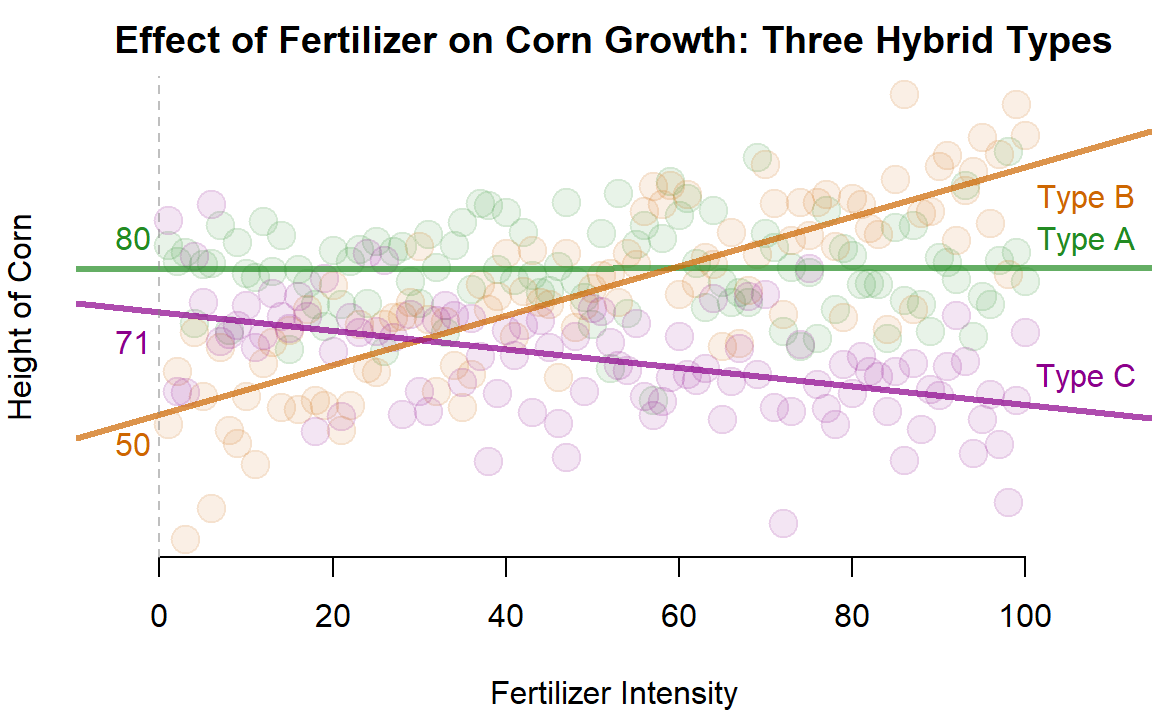
\includegraphics[width=0.7\linewidth]{Foundations_of_Program_Evaluation_files/figure-latex/unnamed-chunk-43-1} \end{center}

\begin{Shaded}
\begin{Highlighting}[]

\KeywordTok{stargazer}\NormalTok{( m}\FloatTok{.04}\NormalTok{, m}\FloatTok{.05}\NormalTok{, m}\FloatTok{.06}\NormalTok{, m}\FloatTok{.07}\NormalTok{, }\DataTypeTok{type=}\StringTok{"html"}\NormalTok{, }
           \DataTypeTok{digits=}\DecValTok{2}\NormalTok{, }
           \DataTypeTok{omit.stat=}\KeywordTok{c}\NormalTok{(}\StringTok{"f"}\NormalTok{,}\StringTok{"adj.rsq"}\NormalTok{,}\StringTok{"ser"}\NormalTok{),}
           \DataTypeTok{intercept.bottom =} \OtherTok{FALSE}\NormalTok{ )        }
\end{Highlighting}
\end{Shaded}

Dependent variable:

height

(1)

(2)

(3)

(4)

Constant

70.80***

79.78***

49.74***

(2.05)

(2.05)

(2.05)

fertilizer

0.11***

-0.19***

0.003

0.51***

(0.03)

(0.04)

(0.04)

(0.04)

dumA

74.51***

8.98***

30.03***

(1.89)

(2.90)

(2.90)

dumB

70.09***

-21.05***

-30.03***

(1.89)

(2.90)

(2.90)

dumC

55.72***

-8.98***

21.05***

(1.89)

(2.90)

(2.90)

fertilizer:dumA

0.19***

-0.51***

(0.05)

(0.05)

fertilizer:dumB

0.70***

0.51***

(0.05)

(0.05)

fertilizer:dumC

-0.19***

-0.70***

(0.05)

(0.05)

Observations

300

300

300

300

R2

0.97

0.59

0.59

0.59

Note:

\emph{p\textless{}0.1; \textbf{p\textless{}0.05; }}p\textless{}0.01

We now have a model that can be used to test whether each hybrid type
responds to fertilizer differently.

Similar to the difference-in-difference models, in order to calculate
the slope for each group we need to add the group-specific slope
component to the main slope, which is associated with the omitted
category.

Again, not that if you change the reference category you will change the
specific model coefficients. But no matter which category is omitted the
models should produce the same group slopes.

You need to take care to interpret statistical significance in reference
to the omitted category. For example, corn Type A does not seem
responsive to this particular fertilizer (the slope is 0). Type C has a
negative response. If we omit Type C from the regression model then the
global slope will represent the response of the omitted category, and
the coefficient for the fertilizer Type A interaction will tell us
whether the slope differs from the reference group. Since A does differ
from C both are signiifcant. But if we omit Type A, now the reference
slope is approximately 0, which will not be statistically significant.

This shows us that the statistical significance of the interaction terms
relate to how they difference from the reference group, not whether they
differ from zero.

\bibliography{book.bib,packages.bib}


\end{document}
